%%%%%%%%%%%%%%%%%%%%%%%%%%%%%%%%%%%%%%%%%%%%%%%%%%%%%%%%%%%%%
%                                                           %
% Cette version repart de 03_Draft\Layoff-short-current.tex %
%                                                           %
%%%%%%%%%%%%%%%%%%%%%%%%%%%%%%%%%%%%%%%%%%%%%%%%%%%%%%%%%%%%%

%\input{preamblemalg1}
\documentclass[12pt,french,american,a4paper]{article}

\usepackage[utf8]{inputenc}
\usepackage{threeparttable}
\usepackage{graphicx}
\usepackage[export]{adjustbox}
\usepackage{pdflscape}



\usepackage{amsmath,amstext,amssymb,dsfont}
\usepackage{setspace}
\usepackage{chngpage}
\usepackage{caption}
\usepackage{subcaption}
\usepackage{placeins}
\usepackage{titling}

\usepackage{ bbold }
%\usepackage{palatino}

\usepackage{textcomp}
\usepackage{courier}
\usepackage{todonotes}
\usepackage{pgffor}
\usepackage{tabularx} 

\renewcommand{\baselinestretch}{1.3}
%\usepackage{lipsum}
%\usepackage{mwe}
\usepackage{rotating}
\usepackage{booktabs}
\usepackage{siunitx}
\usepackage{graphicx}
\usepackage{comment}
\usepackage{eurosym}
\usepackage{amsfonts}
\usepackage{amsthm}
\usepackage{bm}
\usepackage[LGR,T1]{fontenc}
\usepackage[sc]{mathpazo}
\usepackage[round,authoryear]{natbib}

\usepackage{graphicx, color}
\usepackage{url}
\definecolor{NavyBlue}{rgb}{0,0,0.5}
\definecolor{citecolor}{rgb}{.54,0,0}
\definecolor{bgreen}{rgb}{0.05, 0.5, 0.06}
\usepackage{xcolor}
\RequirePackage{titletoc}
\usepackage[colorlinks=true, linkcolor=NavyBlue, citecolor = NavyBlue, urlcolor = magenta, hypertexnames=false]{hyperref}
%\usepackage[colorlinks=true, linkcolor=red, citecolor = citecolor, urlcolor = magenta]{hyperref}
\usepackage{a4wide}
\usepackage{setspace}

\usepackage[scaled]{helvet} 


\newcolumntype{P}[1]{>{\centering\arraybackslash}p{#1}}
\usepackage{lscape}
\setlength{\parskip}{1ex plus 0.3ex minus 0.3ex} 
\setlength{\skip\footins}{1cm} 
\usepackage{enumitem}
\usepackage[hang,flushmargin]{footmisc}
\usepackage{footnote}

\usepackage{threeparttable}
%\usepackage{float}
\usepackage[paper=a4paper,textheight=24cm,textwidth=16cm]{geometry}


%Change in the input environment (quick fix):
\makeatletter
\AddToHook{env/tabular/begin}{\let\input\@@input}
\makeatother


%\usepackage[margin=2.5cm]{geometry}
\usepackage{tabularx}
\usepackage{colortbl}
\usepackage{xcolor}
\usepackage{ulem}
\usepackage{bbm}
\usepackage[capposition=top]{floatrow}

\newcommand{\sym}[1]{#1}
\usepackage{pdflscape}
%\newcommand{\sym}[1]{\rlap{#1}}% Thanks to David Carlisle

%\usepackage[colorinlistoftodos]{todonotes}


%%%%%%%%%%%%%%%%%%%%%%%%%%%%%%%%%%%%%%%%%%%%%%%%%%%%%%%%%%%%%%%%%%
%%%%%%%%%%%%%%%%%%%%%%%%%%%%%%%%%%%%%%%%%%%%%%%%%%%%%%%%%%%%%%%%%%
\title{\textbf{Understanding the Reallocation of Displaced Workers to Firms}}

\author{Paul Brandily%\thanks{Centre for Economic Performance, paul.brandily@psemail.eu} 
\and Camille Hémet\thanks{Paris School of Economics, Université Paris 1 Panthéon-Sorbonne and CEPR, \protect \\
camille.hemet@psemail.eu} \and 
Clément Malgouyres\thanks{CNRS-CREST, IPP-PSE, clement.malgouyres@ensae.fr} \and Patryk Wisniewski\thanks{CREST, ENSAE Paris, Institut Polytechnique de Paris \protect \\ 
\protect \\ 
We thank Richard Audoly, Clément Bosquet, Thomas Breda, Ana Rute Cardoso, Pierre-Philippe Combes, Gabrielle Fack, Florence Goffette-Nagot, Rachel Griffith, François Fontaine, Laurent Gobillon, Francis Kramarz, Miren Lafourcade, Thomas Le Barbanchon, Guy Michaels, Vladimir Pecheu, Roland Rathelot, Gilles Saint-Paul and Sebastian Siegloch, as well as participants at INSEAD - Collège de France brownbag seminar, CREST-ENSAI seminar, Institute for Public Policies (IPP) internal seminar, Université Paris-Saclay (RITM) seminar, PSE macroeconomic workshop, LISER, SOLE annual meeting and TEPP annual meeting for useful comments and discussion. This work is supported by several public grants overseen by the French National Research Agency (ANR-10-EQPX-17 - Centre d'accès sécurisé aux données - CASD, ANR-18-CE22-0013-01, ANR-19-CE26-0004 and the EUR grant ANR-17-EURE-0001), and benefited from CEPREMAP and CREST funding.}}

\date{\today}



%%%%%%%%%%%%%%%%%%%%%%%%%%%%%%%%%%%%%%%%%%%%%%%%%%%%%%%%%%%%%%%%%%
%%%%%%%%%%%%%%%%%%%%%%%%%%%%%%%%%%%%%%%%%%%%%%%%%%%%%%%%%%%%%%%%%%

% CETTE VERSION : Révision EJ

%%%%%%%%%%%%%%%%%%%%%%%%%%%%%%%%%%%%%%%%%%%%%%%%%%%%%%%%%%%%%%%%%%
%%%%%%%%%%%%%%%%%%%%%%%%%%%%%%%%%%%%%%%%%%%%%%%%%%%%%%%%%%%%%%%%%%



% Definitions formerly supplied by the unavailable root Overleaf document.
\pdfminorversion=7
\usepackage{floatrow}
\usepackage{colortbl}
\newcolumntype{Z}{>{\hsize=.5\hsize\linewidth=\hsize}X}
\providecommand{\sym}[1]{\ifmmode^{#1}\else\(^{#1}\)\fi}
% Avoid widening figures beyond the enclosing subfigure or text column.
\setkeys{Gin}{keepaspectratio}
\usepackage{etoolbox}
\AtBeginEnvironment{table}{\singlespacing}
\AtBeginEnvironment{figure}{\singlespacing}
\AtBeginEnvironment{figure*}{\singlespacing}
\setlength{\emergencystretch}{2em}

\begin{document}

\maketitle




\begin{abstract}\singlespacing
We study job displacement in France. In the medium run, losses in firm-specific wage premia account for a substantial share of the overall cost of displacement. However, despite the positive correlation between wage premia and productivity in the cross-section of firms, we find that workers are reemployed by high-productivity, low -labor-share firms. Workers are re-employed by productive firms but this reallocation comes at a cost to workers. We show further that destination firms are less likely to conclude collective wage agreements and have lower participation rates at professional elections. Overall, our results point to a decline in worker bargaining power.

	
	\noindent \textbf{JEL classification}: J63, J31 \\ %J52, L25
	\noindent \textbf{Keywords}: Displaced workers, Wage, Reallocation, Productivity, Labor share.
\end{abstract}



\newpage
%%%%%%%%%%%%%%%%%%%%%%%%%%%%%%%%%%%%%%%%%%%%%%%%%%%%%%%%%%%%%%%%%%
%%%%%%%%%%%%%%%%%%%%%%%%%%%%%%%%%%%%%%%%%%%%%%%%%%%%%%%%%%%%%%%%%%
\section{Introduction}
%%%%%%%%%%%%%%%%%%%%%%%%%%%%%%%%%%%%%%%%%%%%%%%%%%%%%%%
%                                                     %
% Cette version repart de 03_Draft\intro-short-V1.tex %
%                                                     %
%%%%%%%%%%%%%%%%%%%%%%%%%%%%%%%%%%%%%%%%%%%%%%%%%%%%%%%

% NB: Je supprime toutes les (grosses) parties qui étaient en commentaire dans la version précédente pour qu'on y voit plus clair.

Since \cite{Jacobson1993} and \cite{Farber1993}, the literature on job displacement has documented long-run earnings losses following layoffs. This empirical regularity highlights the costs associated with the reallocation of factors of production. While this reallocation process is at the core of productivity growth in modern economies \citep{foster2001aggregate,hsieh2009misallocation}, it can entail substantial {private} costs.

Recent contributions on job displacement emphasize the role of firms in explaining the private cost of this reallocation. In particular, these studies show that displaced workers reallocate to firms with lower wage premia, measured \textit{à la} \cite{Abowd1999} (henceforth AKM). Yet, little is known regarding the productivity and the labor share of those (destination) firms. Productivity and wage premia being positively related across firms \citep[e.g.][]{card2016bargaining}, the reallocation of displaced workers to lower-wage firms appears likely to reflect movements toward lower productivity firms. But it could instead be driven by reemployment at low labor share, high productivity firms \citep{autor2020fall,aghion2022theory}. Both possibilities are compatible with the documented earnings losses but have different implications regarding \textit{i)} the ``productivity-enhancing'' nature of labor reallocation in the wake of downsizing events \citep{foster2016reallocation}, and \textit{ii)} whether earnings losses reflect a decline in workers' negotiation power or reallocation to firms generating less surplus per worker.%\footnote{Here, we simply define loss in negociation power as being re-employed by firms with unfavorable wage policy \textit{given}, as opposed to \textit{because} of, their productivity.}

In this paper, we shed new light on these questions by studying jointly the wage policy and productive performance of the firms in which displaced workers are re-employed. We proceed in three steps. First, using administrative data from France, we study a large set of workers laid-off for economic reasons, and find evidence of large and persistent earnings losses---about a third of pre-displacement earnings 6 years post-displacement (\textcolor{red}{could add results}) \textcolor{orange}{[32\%: $-7{,}961$ euros at $t^D+6$ (Appendix Table A7, col. 2) over the 24,848-euro baseline of Table 1; $-0.322$ in logs]}. Using detailed administrative data on hours worked, we find that working time explains almost all of the short run losses (1 to 2 years post-displacement), but tends to recover in the medium run (5 years post-displacement). By contrast, losses in hourly wage rate, while initially smaller, show no sign of recovery. These persistent losses in hourly wages are explained to a substantial extent (43\% -> \textcolor{red}{37.1\% 5 years after displacement}) \textcolor{orange}{[37\% OK: Table 2, col. 7 at $t^D+5$ = 0.371]} by declines in firm wage premia. Our findings add to an active literature assessing the importance of lost wage premia in shaping the cost of displacement \citep{Gulyas2019,Lachowska2020,moore2019firm,Schmieder2020,fackler2017explaining,bertheau_etal_2023,helm2022}.\footnote{The contribution of firm-specific wage premia to earnings losses remains debated, with some studies finding large effects (e.g. \citealp{Gulyas2019,Schmieder2020}) and others more modest ones (e.g. \citealp{Lachowska2020}); see Section \ref{sec:FEtheory} for further discussion.}

% Alternative with more references, including Bertheaud qu'on nous reprochait de ne pas assez citer, mais du coup comme on va le remettre dans le main, on peut sans doute s'en passer dans la footnote: 
%\footnote{The contribution of firm-specific wage premia to earnings losses remains debated, with some studies finding large effects (e.g. \citealp{Gulyas2019,Schmieder2020}) and others more modest ones (e.g. \citealp{Lachowska2020}); cross-country evidence is provided by \citealp{bertheau_etal_2023}. See Section \ref{sec:FEtheory} for further discussion.}

% original footnote:
%\footnote{The role of firm-level wage premium in overall earnings and wage rate losses of displaced workers is an active topic of research. \cite{Gulyas2019} and \cite{Schmieder2020} find firm premium important for shaping earnings losses, consistent with the work of \cite{goldschmidt2017rise} on outsourced workers. Conversely, \cite{Lachowska2020} find this loss to be of modest importance. \cite{bertheau_etal_2023} provide cross-country evidence. Further literature discussion is in section \ref{sec:FEtheory}.}

In a second step, we investigate the patterns of workers' reallocation in terms of firms' characteristics, such as productivity or labor share. We show that the reallocation of workers to lower-wage-premium firms does not reflect a reallocation towards low-productivity firms. Instead, despite the positive correlation between productivity and wage premia in the cross-section of firms, we find that destination firms tend to be more productive but pay lower premia.\footnote{This result is compatible with \cite{bell_bukowski_machin_2024} who show that the pass-through from rents to wages tends to decline over time, using UK data.} Those firms consequently have much lower labor share. Crucially, this analysis does not assume that displaced and control workers initially work in similar firms. Rather, it exploits exogenous displacement from the workers' perspective, and studies its consequences in terms of reallocation. Furthermore, we use pre-displacement measures of firms' characteristics to ensure they do not reflect post-layoff dynamics. Overall, we view this pattern as suggesting that losses in premia reflect a decline in bargaining power as opposed to difficulties to access jobs in productive firms. Finally, we strengthen the case for a loss in bargaining power by examining two additional qualitative outcomes that capture the state of labor relations at the firm level. We show that displaced workers are reemployed by firms that \textit{i)} are less likely to reach firm-level collective wage agreements and \textit{ii)} have lower turnout in professional elections. 

We contribute to the literature in three main ways. First, thanks to an administrative definition of economic layoffs, we are able to focus on a larger set of involuntary separations and a more representative set of firing firms (``origin firms'' henceforth) than what is captured in the extant literature relying on mass layoffs. Crucially, we show that our set of origin firms are more representative in terms of wage premia, so that losses in premia following displacement are less likely to be driven by mean-reversion.\footnote{See \cite{Schmieder2020} section IV.A on mean reversion in establishment premia loss. } While the qualitative reallocation pattern documented above---displaced workers moving to firms with higher productivity but lower wage premia and lower labor shares---is preserved when we implement a mass-layoff design, we find that the share of the hourly wage losses explained by wage premium losses is larger in the mass-layoff sample, presumably because that design oversamples higher-premium origin firms. Second, %taking advantage of the possibility offered by French data to 
linking matched employer-employee data with exhaustive accounting data on firm performance, we compare losses in wage premia with measures of productivity, surplus per worker and labor share of the destination firms. To the best of our knowledge, we are the first to carry out this data intensive exercise when studying job displacement.\footnote{\cite{haltiwanger2018moves} study workers flows and firm productivity but focus on the reallocation of workers through job-to-job moves and do not study AKM-type wage premia. Closer to our exercise are \citet{haltiwanger2018cyclical} and \citet{bertheau_vejlin_2023}, who study worker flows across firms classified by average wage and labor productivity over the business cycle.} It reveals that destination firms are both more productive and lower labor share firms.
This finding speaks to random-search models of the labor market \citep{Lentz2024}. In these models, workers climb a job ladder via on-the-job search, moving to higher-surplus firms or renegotiating their wage upward when outside offers arrive, while displacement pushes them back down the ladder. The AKM firm wage premium $\psi_f$ identifies a firm-specific component of wages common to all workers of the firm. Structural displacement models in this class such as \citet{krolikowski2017job} and \citet{Audoly_2024} attribute the firm-side wage losses to reallocation toward less productive firms. Our findings point to a more nuanced picture: re-employed workers move \emph{up} the productivity distribution but \emph{down} the wage-premium distribution. The estimation and calibration of such models would therefore benefit from using direct productivity data and contrasting their results against the empirical pattern of reallocation along the productivity distribution. Finally, we assemble new data to corroborate the idea that earnings losses associated with displacement reflect a loss in collective bargaining. We build original firm-level indicators capturing the state of labor relations in each employer, in the pre-displacement period. The use of firm-level data (as opposed to sector-level proxies for collective bargaining) is crucial as we show that our effects are driven by within-sector dynamics. We provide evidence that displaced workers are reallocated to employers that are less likely to successfully conclude firm-level collective wage agreements and where workers have a lower participation rate during professional elections---arguably reflecting a lower degree of organization of the workforce.


%\todo[inline]{Emphasize novelty: lower issue of mean reversion because more representative of broad set of separations.}



\FloatBarrier
%%%%%%%%%%%%%%%%%%%%%%%%%%%%%%%%%%%%%%%%%%%%%%%%%%%%%%%%%%%%%%%%%%
\section{Data, sample construction and institutional setting} \label{sec:Data} 
%%%%%%%%%%%%%%%%%%%%%%%%%%%%%%%%%%%%%%%%%%%%%%%%%%%%%%%%%%%
%                                                         %
% Cette version repart de 03_Draft\data_current-short.tex %
%                                                         %
%%%%%%%%%%%%%%%%%%%%%%%%%%%%%%%%%%%%%%%%%%%%%%%%%%%%%%%%%%%

% NB: Je supprime toutes les (grosses) parties qui étaient en commentaire dans la version précédente pour qu'on y voit plus clair.

\subsection{Data}
Throughout the paper, we rely on several French administrative sources. We first use linked employer-employee datasets (Panel DADS and FH-DADS) to identify workers, their job (wage, hours, employer) and layoff. Panel DADS is a random sample of 1/12 of the universe of workers, and FH-DADS matches this panel with unemployment insurance administrative records. 
% , we observe firm's unique, time-invariant identifier (SIREN code), which allows us to retrieve firms' balance-sheet and income statement from the FICUS-FARE datasets. 
We also use the exhaustive version of the linked employer-employee data, DADS Postes, to estimate firm fixed effects. %in section \ref{sec:data:firm:premium}
Firms' balance-sheet and income statement are retrieved from the FICUS-FARE administrative dataset, built from the corporate tax returns and the social security declarations of the universe of firms in the non-financial corporate sector. All datasets are merged through the firm identifier (SIREN).\footnote{See Appendix Table \ref{apptab:datasets} for more details about data.}
%In the remainder of this section, we explain how we build our samples and how we measure our main outcomes of interest. Appendix Table \ref{apptab:datasets} provides more details about our datasets.


\subsection{Displaced workers}  
\label{sec:data:displaced}


%n our main sample, we follow workers laid-off for economic reasons (\textit{licenciés économiques}, LE hereafter) between 2002 and 2012. 
We identify workers laid-off for economic reasons (\textit{licenciés économiques}, LE hereafter) using FH-DADS data, which matches: \textit{i)} a panel of workers with data on wages, hours, and employer (panel DADS) and \textit{ii)} unemployment insurance data with details on unemployment spells (registration date, duration, benefits). Crucially, this dataset, which covers the period from 2002 to 2012, precisely identifies LE workers by documenting the reason for registration at the French employment agency (e.g., layoff for personal vs. economic reasons) as declared by the firm to the administration.

Economic layoffs require firms to justify economic difficulties, as detailed in Appendix \ref{appsec:LE_def}. Given the strict legal definition and conditions, firms are unlikely to misdeclare personal layoffs as economic ones, despite potential incentives (\cite{fraisse2015labor} document that personal dismissals are more often contested in court).\footnote{Supporting this, \cite{signoretto2019individual} find that economic dismissals are largely explained by firms' economic conditions, while personal layoffs are linked to management style.}

Focusing on a sample of LE workers has two main advantages. First, it minimizes the risk of including individuals who voluntarily left their firm before or during a mass layoff. This concern has been emphasized by \cite{seim_2019}, who quantifies the bias resulting from not being able to separate quits from layoffs (\textit{e.g.} focusing on workers leaving the firm within a time window of an important downsizing of the labor force). Moreover, because economic layoffs in our setting are legally defined and reported by firms to the administration, our measure reflects the circumstances of separation rather than inferring displacement indirectly from firm-level employment changes. In this respect, our approach is related to other recent efforts to move beyond canonical mass-layoff definitions, including \cite{seim_2019,fackler2017explaining,cederlof_2024} and \cite{bertheau_etal_2023}.\footnote{Importantly, workers laid off for economic reasons are eligible for the standard unemployment insurance scheme applicable to all involuntarily displaced workers in France, with no specific difference in benefit generosity or access to labor market programs relative to other forms of layoffs; we provide further institutional details in Appendix \ref{appsec:LE_def}}

% NB, Seim 2019 dit :
% Finally, by using administrative data on displacements, it is possible to assess quantitatively the bias that results from previous studies not being able to separate quits from layoffs.
%The final part of the paper addresses the potential bias that might plague previous studies of effects of job loss that use matched employeremployee data and thus are unable to distinguish quits from layoffs. I use the Swedish employer-employee records and define separations of matches as job displacements according to the literature. Estimates from regressions using conventional approaches are compared with the estimates obtained when using the PES data, where displacements are directly observed. I do not only assess the potential bias in previous studies, but also propose how to define separations as displacements in the absence of direct data on job displacements. First, separations in periods of mass separations are defined as displaced, following e.g. (Jacobson et al., 1993) and (Sullivan and von Wachter, 2009). The mass layoff estimates turn out to significantly understate the effects of displacement. Instead, defining separations in three-year time windows prior to plant closure as displacements leads to an overestimation of the effects. The arguably most accurate estimates are obtained by defining displacements as separations occurring during a one-year window preceding plant closure.

Second, it allows for a more representative set of employers compared to the literature on mass layoffs, which typically defines them as a 30\% or more decline in labor force \citep[e.g.][]{Jacobson1993,Gathmann2018,Gulyas2019,Lachowska2020,Schmieder2020} and imposes a minimum-firm-size restriction (often $\geq 50$ employees). We deliberately do not impose such a size threshold: rather than firm size in headcount terms, the relevant dimension for our analysis is firm wage-setting, which we summarise with the AKM firm fixed effect. Along this dimension, our LE sample is closer to the population firm-premium distribution than the typical mass-layoff sample, which selects on relatively large and high-premium employers (Appendix Figure \ref{fig:sample_FEdist}).
% This footnote is now in the main text in the "rob test" subsection.
%\footnote{As noted by a referee, in small firms, firm-level difficulties may still partly reflect the performance of individual workers, so that layoffs classified as economic may in practice be related to worker-specific factors. Figure \ref{fig:wage_decomposition_size10} shows that our main results are robust to restricting our sample to firms with more than 10 workers.}

To ensure our sample definition is not the sole driver of results, we build a second sample based on mass layoffs (MLO): plants losing at least 30\% of employees. This approach aligns with the literature and allows for comparison with prior studies. Appendix \ref{appsec:mlo} provides details on this sample.

\paragraph{Construction of the treatment (LE workers) and control groups.} 

The year of layoff, denoted $t^D$, is when the individual registers for unemployment after an economic layoff. We define a LE worker's previous job as the position with the end date closest to the contract end date recorded by the unemployment agency. We focus on individuals losing stable jobs, selecting workers aged 20-50 at layoff %, who worked over 1800 hours in the previous job in $t^D-1$ and $t^D-2$, 
and who are not employed in the same firm on June 30, $t^D+1$. In addition, we impose a three year tenure condition, so as to analyze a sample of workers with a strong labor market attachment: LE workers must be observed in the firm at least on $t^D$, $t^D-1$ and $t^D-2$.\footnote{The first LE that are included in our analysis are observed in 2005.} % The latest LE workers that are included in the analysis are observed in 2012, but for them we do not have any "post-layoff" observation.
An individual is included only when first registered as LE and meeting these criteria. Overall 20,897 -> \textcolor{red}{21,132} individuals, displaced from 14,038 -> \textcolor{red}{14,115} distinct firms, fit these criteria. \textcolor{orange}{[21,132 and 14,115 OK: Table 1, last two rows]}
 
We use propensity score matching to construct a control group for LE workers. Matching is performed on all non-displaced workers in FH-DADS who meet the criteria applied to the LE workers in terms of job tenure. %and hours worked. 
Matching occurs within year and sector-size cells, defined by the intersection of 10 industries (1-digit) and 4 quartiles of firm size (based on the size distribution at $t^D-1$ -> \textcolor{red}{$t^D-2$} among LE). We match workers using age, firm size at $t^D-2$ -> \textcolor{red}{$t^D-1$} \textcolor{orange}{[$t^D-1$ OK: Table 1 row ``\# employees at firm at $t^D-1$''; the quartiles of the size distribution at $t^D-2$ cannot be checked against a table]}, and hourly wage and hours worked in the main job in $t^D-2$ and $t^D-3$. Using pre-displacement characteristics measured sufficiently far in advance helps limit the risk that these variables are already affected in the period immediately preceding displacement. We estimate a probit to predict the propensity score and keep the nearest neighbor, with replacement. The LE panel (LE workers and their control group) is described in Section \ref{sec:stat_desc}.\footnote{Our control group consists of workers who are never displaced through either an LE or an MLO30 event over the sample period; we do not require controls to remain continuously employed at the same firm over the post-event window---in line with \citet{Schmieder2020}, \citet{Lachowska2020} and \citet{bertheau_etal_2023}, and departing from the convention of \citet{Jacobson1993}. Appendix~\ref{app:stayer_controls} re-estimates the main results on the MLO30 sample using the JLS-style stayer control group, as a comparability check with the existing literature.}

\subsection{Firm wage premia}
\label{sec:data:firm:premium} 

We compute firm wage premia using the exhaustive version of the matched employer-employee data (DADS \textit{postes}). This version of DADS allows us to estimate firm fixed effects for a larger set of firms compared to studies focusing on the worker-level panel \citep[e.g.][]{Abowd1999,bertheau_etal_2023} which is a 1/12th sample of the exhaustive file. In the exhaustive dataset, worker identifier is renewed at each vintage but any vintage $t$ contains information on jobs at time $t$ and $t-1$. Following \cite{godechot2023akm}, we take advantage of this overlap, using common individual information between vintage $t$ and $t-1$ in order to build a new worker panel based on the exhaustive data, which covers about 98\% of all workers between 2002 and 2015.

The DADS \textit{postes} presented here and the panel DADS cannot be merged at the worker-level. This implies that we cannot recover worker fixed-effects. We view this limitation as innocuous as we are primarily interested in the role of firms characteristics in explaining the cost of displacement---unlike for instance \citep{helm2022} who study how this effect varies with worker-fixed effect.

The AKM-type model we fit writes as follows:
\begin{equation}\label{eq:akm_basics}
	\ln \left(w_{it}\right)=\psi_{J(i, t)}+\alpha_{i}+\lambda_{t}+\epsilon_{i t}, 
\end{equation}
where $w_{it}$ refers to worker $i$'s  hourly wage in year $t$, \textcolor{red}{winsorized within year at 1\%/99\%} \textcolor{orange}{[OK: the AKM code winsorizes the hourly wage at 1/99 year by year]}, $\psi_{J(i, t)}$ is the fixed effects of firm $J$ where worker $i$ was employed at period $t$ and where $\alpha_{i}$ and $\lambda_{t}$ are individual and time fixed effect respectively. The period used to estimate firm fixed effects covers years 2002 to 2015.

To limit contamination of firm fixed effects by displacement-induced worker reallocation, we exclude from the AKM estimation sample all post-event observations of workers leaving an LE or MLO firing firm in the year of the event or the year after, while retaining their pre-event observations. Because the worker identifiers used in the event-study sample (\textit{panel DADS}) cannot be directly linked to those used in the exhaustive matched employer--employee data (\textit{DADS postes}), this exclusion is implemented at the firm-year level rather than for displaced workers in our estimation sample only. Concretely, any worker leaving an LE or MLO firm in year $t^D$ or $t^D+1$ is excluded from the AKM sample from that point onward. This procedure follows the logic of the contamination corrections, which typically exclude post-displacement observations from the AKM estimation sample.\footnote{Recent studies have emphasized that displacement-induced worker reallocation can contaminate AKM firm fixed effects if post-displacement observations are included in the estimation sample. \citet{Lachowska2020} exclude displaced workers entirely from the AKM estimation sample, while \citet{moore2019firm} and \citet{Schmieder2020} exclude post-layoff observations only. Our approach is closest in spirit to the latter studies, although the absence of a direct worker-level link between \textit{panel DADS} and \textit{DADS postes} requires implementing the exclusion at the firm-year level.} However, our exclusion rule is more stringent than in the existing literature, since it applies to all workers leaving LE or MLO firms rather than only to displaced workers included in the event-study sample.

Firm and worker fixed effects have been shown to suffer from limited mobility bias \citep{andrews2008high}, which implies an upward bias on the estimate of the variance of firm fixed effects and a downward bias regarding the covariance between worker and firm fixed effects. Our use of the near universe of across-firms movement tempers this risk. Moreover, this type of bias is particularly relevant when studying assortative matching \citep{bonhomme2019distributional} or the contribution of firm to wage dispersion \citep{song2019firming}. %{Recent contributions have proposed either alternative estimation framework to the AKM two-way fixed effect approach \citep{bonhomme2019distributional,bonhomme2020much} or corrections applied to the variance and covariance estimator \citep{kline2020leave}.} 
In this paper, however, we are interested in the first moment of these firm fixed effects. Accordingly, measurement error occurs in our dependent variable and is likely to affect the precision of our estimates but not to bias them in any systematic way.\footnote{Recent work on French data corroborates this assessment for long panels: both \citet{godechot2023akm} and \citet{milsom_hou_2024} find that the Kline-Saggio-S{\o}lvsten correction for limited mobility bias is small in magnitude when AKM is estimated over time spans similar to ours, leaving the first moment of the firm fixed effects essentially unaffected. \textcolor{orange}{[reference check, 2026-11-20: neither paper reports this. \citet{godechot2023akm} use a split-sample correction, not KSS, and find significant differences between corrected and uncorrected variance components; Milsom and Hou's French sample covers 2015--2019, their paper is titled ``Do Workers Sort to Firms or to Occupations?'', and no paper with the cited title exists. Proposed: ``Limited mobility bias affects quadratic functions of the estimated firm effects, such as their variance or their covariance with worker effects \citep{andrews2008high}, but the estimated effects themselves are unbiased \citep{godechot2023akm}. Since our outcome is the firm effect itself, the bias adds noise to the dependent variable without shifting the event-study coefficients.'' Then drop Milsom and Hou.]}}


\subsection{Other firm characteristics}
\label{sec:data:firm:other}

We measure labor productivity and labor share using the FICUS-FARE database, as processed by \citet{burstein_etal_2025} (see Appendix Table \ref{apptab:datasets}). We build two productivity measures: value added per worker, and a measure adjusted for capital intensity. The latter is the residual of a regression of value added on (tangible capital and employment) -> \textcolor{red}{log tangible capital and log employment} \textcolor{orange}{[OK: the code regresses log VA on log employment and log tangible fixed assets, demeaned by year; it also runs the regression separately by 2-digit sector, which the text does not say]} with year fixed effects. More sophisticated total factor productivity measures are feasible but they are highly correlated with simple OLS-based estimates \citep{van2012total} and therefore unlikely to change our results. We compute labor share as the ratio of total labor costs to value added.

Our main analysis measures firm-level productivity and labor share as three-year averages centered on $t^D_i-4$ (i.e.\ over $t^D_i-5$, $t^D_i-4$ and $t^D_i-3$). For each displaced worker this is a fixed pre-displacement window relative to the worker's own event year, so our estimates reflect displacement-induced reallocation of workers to firms with different initial productivity rather than within-firm changes following the layoff. As a robustness exercise, we also recompute firm-level outcomes as within-firm averages over the full 2002--2015 period (Appendix Figures~\ref{fig:prod_et_al_Full_LE} and \ref{fig:prod_et_al_Full_MLO}); the qualitative pattern is preserved and quantitatively amplified.


\subsection{Descriptive statistics on the estimating sample} 
\label{sec:stat_desc}
Our main sample consists of 42,264 individuals equally distributed among treated and control individuals. Standard descriptive statistics on the quantitative variables used in the matching process are reported in Table \ref{tab:desc:AllLE}, where all variables are measured before displacement. Displaced individuals at baseline are 37 years old on average, earn 15.27 euros per hour and worked 1,594 hours. As expected given the matching procedure described above, these variables are well balanced across groups: the Imbens-Rubin normalized difference reported in column (3) never exceeds 0.25, in line with \citet{rubin_assessing_2015} rule of thumb. %suggesting that the matching procedure is successful in reaching balance along matching variables. 

Table \ref{tab:desc:AllLE} also reports the distribution of quantitative variables that were not used in the matching process. About 60\% of the sample are males. They earned about 24,800 euros when considering all their contracts. We also see that the two groups were, on average, employed in similar type of firms in terms of the 2002-2015 wage premia of the pre-layoff employers. %-- estimated from the AKM framework using exhaustive data of firms over the 2001-2015 period
% with godechot, starts in 2002
 In these dimensions as well, both treated and control groups look similar according to the Imbens and Rubin normalized difference. %Here again, none of the differences in distribution seems to exceed Rubin and Imbens rule of thumb. 

Figure \ref{fig:desc:LEquali} finally displays the distribution of LE workers by categories of sector of employment (\ref{fig:desc:LEsec}), occupation (\ref{fig:desc:LEocc}) and highest diploma (\ref{fig:desc:LEdip}). Sector is a matching variable so the displaced and control distributions coincide at $t^D-1$ by construction; we therefore plot the control group only and label it as the \textit{estimation sample}, with the broader DADS panel population shown for reference. Occupation and educational attainment are not used in the matching algorithm and are displayed as a Displaced-vs-Control comparison; both are well balanced. One year before layoff, displaced and control workers mainly worked in manufacturing and extraction or the retail sectors and a large share were blue collars or clerical workers. Compared to the broader DADS panel, our estimation sample is over-represented in manufacturing and construction and under-represented in services to firms and public/education/health, reflecting the sectoral incidence of LE events. %(called ``intermediate professions'' in the French classification) or employees. 
The information about diploma is missing for a large part of the sample (and we exclude it from further analysis) but the balance among observed individual remains (with the highest observed share being vocational basic training). Overall we reach a satisfactory level of balance across both matched and unmatched variables (as is usual in the job displacement literature).  



\FloatBarrier

%%%%%%%%%%%%%%%%%%%%%%%%%%%%%%%%%%%%%%%%%%%%%%%%%%%%%%%%%%%%%%%%%%
\section{Earnings losses and the role of firm wage premia} \label{sec:FEtheory}
%%%%%%%%%%%%%%%%%%%%%%%%%%%%%%%%%%%%%%%%%%%%%%%%%%%%%%%%%%%%%
%                                                           %
% Cette version repart de 03_Draft\rolefe_current-short.tex %
%                                                           %
%%%%%%%%%%%%%%%%%%%%%%%%%%%%%%%%%%%%%%%%%%%%%%%%%%%%%%%%%%%%%

% NB: Je supprime toutes les (grosses) parties qui étaient en commentaire dans la version précédente pour qu'on y voit plus clair.


\subsection{Empirical specification}\label{sec:empirical}

We analyze the cost of job displacement by estimating the following equation:
\begin{equation}\label{eq:main_estimating_equation}
Y_{it} = \sum\limits_{d=-2}^{6} \beta_{d} \times {\mathbbm{1}}\{t^D_i+d=t\} \times \mathbbm{1}\{D_i=1\} + \sum\limits_{d=-3}^{6} \delta_{d} \times {\mathbbm{1}}\{t^D_i+d=t\} + \alpha_i + \delta_t + \epsilon_i,
\end{equation}

where $Y_{it}$ is an outcome of interest measured in year $t$ for individual $i$ employed in firm $J(it)$, displaced in year $t^D_i$. $\beta_{d}$ measures the change in $Y$ for displaced workers (indicated by $D=1$) compared to the control group, $d$ periods after displacement. The model includes worker ($\alpha_i$) and year ($\delta_t$) fixed effects. In these estimations, we take $t^D-2$ as the reference year, as outcomes may already be affected in the year prior to displacement ($t^D-1$). Standard errors are clustered at the individual level.\footnote{We use a matching procedure with replacement: non-displaced individuals may enter the control group multiple times if they are the best match for several displaced workers. In this case they will appear under different ``worker'' identities. We cluster standard errors at the true ``individual'' level however to account for the dependence between observations that this may introduce. }

\subsection{Total earnings and employment}\label{sec:earnings_employment} %and hours worked
We first establish the impact of displacement on earning and employment, including adjustment at the extensive margin. Table \ref{tab:evstudytable_body} reports the coefficients $\beta_{d}$ from different estimations of equation (\ref{eq:main_estimating_equation}).\footnote{Throughout this section, the headline coefficients on hours and earnings are reported in log points; these should be read as approximate level percentages only when small. The largest coefficients we report ($-0.939$ on log earnings and $-0.961$ on log hours at $t^D$ -> \textcolor{red}{-0.932 / -0.953} \textcolor{orange}{[OK: Table 2, cols. 3--4 at $t^D$]}) correspond to level drops of $1-\exp(-0.939) = 60.9\%$ and $1-\exp(-0.961) = 61.7\%$ \textcolor{orange}{[$1-\exp(-0.932)=60.6\%$ and $1-\exp(-0.953)=61.4\%$]} respectively, not to the near-elimination of earnings that the log values might suggest if read linearly. The level specification in column~(2) of Table~\ref{tab:evstudytable_body} provides a direct check: the earnings effect at $t^D$ is $-14{,}062$\EUR{} -> \textcolor{red}{13,731} \textcolor{orange}{[OK: Table 2, col. 2 at $t^D$]} on a control-group mean of $25{,}425$\EUR{} -> \textcolor{red}{25,710} \textcolor{orange}{[control mean not in any table; 13,731/25,710 = 53.4\% is arithmetically right]} at the same horizon, a $55.3\%$ -> \textcolor{red}{53.4\%} drop, in line with the log estimate.} In columns (1) and (2), the outcome variable is employment status and overall earnings, respectively. Because outcomes are measured at the annual level and displacement occurs within the year, estimates at $t^D$ reflect a mix of pre- and post-displacement outcomes and therefore understate the full effect, which is more accurately captured at $t^D+1$. The results show the well-known losses following displacement: employment probability falls by about 32 percentage points at $t^D+1$ (relative to the control group), then progressively attenuates over time to about $-14$ percentage points after five years. This fall drives a decline in annual earnings that culminates (\textcolor{red}{false: it doesn't culminate, so either we go to 0 or change the phrasing}) \textcolor{orange}{[Table 2, col. 2: $-13{,}731$ at $t^D$, $-13{,}687$ at $t^D+1$, $-8{,}690$ at $t^D+5$; proposed: ``This fall drives a decline in annual earnings of about 13,700 euros in the year following displacement (55\% of the baseline annual earnings of Table 1), which attenuates to about 8,700 euros (35\%) at $t^D+5$.'']} one year following displacement at about \euro 13,900 -> \textcolor{red}{13,687} \textcolor{orange}{[OK]} (39\% -> \textcolor{red}{55\%} \textcolor{orange}{[OK: 13,687/24,848]} of the baseline annual earnings of Table \ref{tab:desc:AllLE}) and attenuates to about \euro 8,700 -> \textcolor{red}{8,670} \textcolor{orange}{[8,690: Table 2, col. 2 at $t^D+5$]} (25\% -> \textcolor{red}{35\%} \textcolor{orange}{[OK: 8,690/24,848]} of baseline earnings) at $t^D+5$. Appendix Figure \ref{fig:aveffect_emp_earn} display those results and associated pre-trends. Figures \ref{fig:raw_mean_earnings} and \ref{fig:raw_mean_hours} present the raw means for each group. 

\subsection{Decomposition of earnings losses}\label{sec:decomposition_losses}
We now decompose earnings losses into hours-worked losses and hourly-wage losses, and further decompose hourly-wage losses, within the AKM framework, into a firm wage-premia component and a residual component. As is standard in the literature, we focus on re-employed workers. This conditioning matters for interpretation: displaced workers are 22 percentage points less likely to be employed than their controls at $t^D+2$, and still 14 points less likely at $t^D+5$ (Table~\ref{tab:evstudytable_body}, column 1), so the estimates below are computed on a selected sample, whose composition changes over time as workers who return to work later progressively enter it. The hourly-wage loss is nevertheless stable between $t^D+2$ ($-0.106$) and $t^D+5$ ($-0.101$), while the loss in firm premia grows from $-0.029$ to $-0.037$, which suggests that later entrants earn about as much per hour as earlier ones, but in firms paying lower premia. Figure \ref{fig:fe_current_event} displays the various elements of this decomposition: losses in total earnings, hours worked, hourly-wage and firm premia. Earnings and hours (in log) drop abruptly and slowly recover. The hours margin, even conditional on being re-employed, remain very strong. This highlights the importance of working with data on hours to assess properly the relative contribution of labor supply and wage rate to the overall earning response.  Interestingly, the effect on hourly wage stabilizes in the medium run at around -0.10, so its contribution to overall loss in earnings grows over time.\footnote{We also observe a counter-intuitive yet familiar bump immediately after the layoff, driven by severance payment, delayed pay and potential measurement error in hours worked.} This finding is in line with recent research on displacement in other countries or over different periods, such as \cite{Lachowska2020} or \cite{Gulyas2019}. While \cite{Schmieder2020} show evidence of a recovery in \textit{daily} wage rate, they also find that the contribution of wage rate decline to overall earnings loss grows over time. (\textcolor{red}{main decomposition isn't same sample, we exported it (it's called sample\_nonmiss in main results) but we never used it beside I think in ref reports?})

\paragraph{Contribution of employer premia to losses in wage rates.} We assess the importance of the loss in firm-specific wage premia using the firm fixed effect as a dependent variable in our main model (equation \ref{eq:main_estimating_equation}). Coefficients are reported in Figure \ref{fig:fe_current_event}. In line with most of the literature, we find that displaced workers re-employ in (relatively) worse-paying firms. By $t^D+5$ the average loss in premium reaches {-0.072} -> \textcolor{red}{-0.037 (note: 7.2 is from the first paper version, no?)} \textcolor{orange}{[$-0.037$ OK: Table 2, col. 6 at $t^D+5$; the $-0.072$ was already stale in R1, whose table had $-0.042$]}. 


To assess the contribution of firm wage premia to losses in hourly wages, \cite{Lachowska2020} compute the ratio of the decline in log firm premia to the total decline in log hourly wages and find a contribution of 17\%.
 %\footnote{These comparisons are built from \cite{Lachowska2020}, Table 2.} 
 We replicate this exercise in column (7) of Table \ref{tab:evstudytable_body}: loss in premia explains 43\% -> \textcolor{red}{37.1\%} \textcolor{orange}{[OK: Table 2, col. 7 = 0.371]} of hourly wage loss at $t^D+5$. Although our estimates of total hourly wage losses at $t^D+5$ are roughly comparable across the two studies (around -10\%), we find that losses in firm wage premia contribute substantially more to hourly wage losses in our context.
 As we also happen to find larger earnings losses than \cite{Lachowska2020}, the contribution of premium loss to earnings loss at $t^D+5$ that we obtain for the LE sample (14\% -> \textcolor{red}{11.8\%, yay!} \textcolor{orange}{[11.6\% with the rounded Table 2 values (0.037/0.318); 11.8\% only if computed from unrounded coefficients---confirm]}) is close to theirs (12\%).\footnote{We find stronger total earnings and hours effects than \cite{Lachowska2020}. At $t^D+5$, log earnings in the LE sample (respectively, MLO30) decrease by $-0.304$ ($-0.159$) -> \textcolor{red}{-0.316 (-0.159)} \textcolor{orange}{[$-0.318$ ($-0.159$): Table 2, col. 3 and Appendix Table A12, col. 3 at $t^D+5$]} and log hours by $-0.223$ ($-0.090$) -> \textcolor{red}{-0.231 (-0.091)} \textcolor{orange}{[OK: Table 2, col. 4; Appendix Table A12, col. 4]}, as compared to $-0.164$ and $-0.047$ in \cite{Lachowska2020}. This can be explained by three important differences between our setting and theirs: \textit{i)} they identify treated workers using mass separations during the $2008$--$2010$ Great Recession; \textit{ii)} they identify displacements through a $30\%$+ employment drop at the firm level and \textit{iii)} their controls are required to remain at the same firm with continuous employment over the post-event window.}
\cite{Schmieder2020} find a substantially larger contribution of firm premia to daily wage losses, around 76\%.\footnote{Table 3 of \cite{Schmieder2020} provides estimates of losses in log daily wages and firm wage premia: 76.3\% (6.94/9.09) in recessions and 75.5\% (3.91/5.16) in booms. Interestingly, although wage losses differ between booms and recessions, the contribution of firm premia (our main object of interest) appears stable over the cycle.} In a contemporaneous work, \citet{bertheau_etal_2023} find that, across seven European countries, firm premia account for 35 to 100\% of the wage loss. Our 37\% figure for the LE sample lies at the lower end of this range. Our MLO30 estimate (63\%), which relies on a mass-layoff design close to theirs, is near their estimate for France (68\%). Since both studies remove displaced workers' trajectories from the AKM estimation sample, the lower LE figure is unlikely to reflect contamination of firm premia; it is consistent instead with LE workers coming less often from high-premium firms (Appendix Figure~\ref{fig:sample_FEdist}). The remaining gap may also reflect differences in wage concepts (daily versus hourly), in job-loss definition (economic versus mass layoffs), or in data source (exhaustive DADS \textit{postes} versus the 1/12 sample for estimating firm wage premia). They discuss the comparison with our paper in their Appendix C3.

Overall, this analysis shows that losses in firm premia are an important driver of decline in hourly wage in the wake of job displacement, and that reallocation to low-wage firms appears quantitatively relevant in our setting in line with recent work in European context \citep[e.g.][]{Gulyas2019,Schmieder2020}.


\subsection{Robustness tests and additional results}
\label{sec:robustness}

We begin by addressing concerns related to the identification of economic layoffs in small firms. In such firms, firm-level difficulties may partly reflect the performance of individual workers, so that layoffs classified as economic may in practice be related to worker-specific factors. Figure \ref{fig:wage_decomposition_size10} shows that our main results are robust to restricting the sample to firms with (more than) -> \textcolor{red}{at least} \textcolor{orange}{[OK: the caption of the corresponding appendix figure says ``at least 10 employees'']} 10 workers.

We then assess the sensitivity of our results to the construction of AKM firm wage premia. Appendix Table~\ref{tab:paper_R_evstudy_god2} and Figure~\ref{fig:paper_R_wage_decomposition_god2} reproduce our results using an unrestricted AKM specification that does not exclude post-displacement observations from the AKM estimation sample. Consistent with the contamination concerns emphasized in the literature, the unrestricted AKM yields substantially larger estimated losses in firm wage premia, although the overall qualitative patterns remain unchanged.

\paragraph{Time variation in firm wage premia.} We estimate firm wage premia over 2002--2015 and treat them as fixed firm characteristics. Firm pay policies do move over time \citep{lachowska2023drift,engbom2023firmpay}, although \citet{lachowska2023drift} find them to be highly persistent. To check that our results do not hinge on the estimation window, Appendix Figure~\ref{fig:akm_windows} re-estimates the premia over five sub-periods (2002--2005, 2002--2010, 2005--2010, 2005--2015 and 2010--2015) and re-runs the event study with each. The loss in firm wage premia appears in every window, with the same timing. At $t^D+5$, it ranges from $-0.027$, with premia estimated over 2002--2005, a window that largely predates the displacement events, to $-0.046$, with premia estimated over 2005--2010, against $-0.037$ in the baseline.

Next, we replicate our analysis using the mass-layoff sample (MLO30) in Figure \ref{fig:fe_current_event_mlo_pretrends}. We find qualitatively similar patterns in terms of earnings and hourly wage losses. At \(t^D+5\), hourly wage losses are \(-0.070\) in the MLO30 sample versus \textcolor{orange}{\(-0.101\)} in the LE sample. Losses in firm wage premia explain around \textcolor{orange}{\(63\%\)} of hourly wage losses at \(t^D+5\) in MLO30 (versus \textcolor{orange}{\(37\%\)} in LE), a reversal that reflects the over-representation of larger and higher-premium firms in the mass-layoff design. %The MLO sample also provides a longer observation window, allowing us to verify that losses in firm wage premia persist up to \(t^D+8\).

These differences across samples are consistent with differences in sample composition. Displaced workers in MLO30 tend to originate from larger and higher-premium firms than those in LE, in line with the over-representation of large firms induced by the mass-layoff design. Appendix Figure~\ref{fig:sample_FEdist} reports the distribution of pre-displacement firm fixed effects in our two samples and across previous studies, and suggests that the LE sample is somewhat less skewed toward high-premium firms.\footnote{In the top two quintiles of the AKM distribution, the share of displaced workers is \(55.9\%\) in LE and \(67.7\%\) in MLO30 \textcolor{orange}{[53.9\% and 65.8\%, as printed on the R2 version of Appendix Figure~\ref{fig:sample_FEdist}; the 67.7\% of \citet{bertheau_etal_2023} below is unchanged]}; the corresponding shares are \(67.7\%\) in \citet{bertheau_etal_2023}, \(61.8\%\) in \citet{Lachowska2020}, and \(75.9\)--\(76.8\%\) in \citet{Schmieder2020} (recession and boom).}

Finally, we re-estimate the wage decomposition separately for men and women in the LE sample (Appendix Figure~\ref{fig:fe_current_event_by_sex}). The two profiles are quantitatively similar across all four outcomes: at \(t^D+5\), the hourly-wage scar is \(-0.105\) for men versus \(-0.089\) for women, while the AKM firm-premium scar is \(-0.041\) versus \(-0.045\). The reallocation patterns we document are therefore not driven by either sex. (\textcolor{red}{note to me (pw): numbers to swap, including at figure A7}) \textcolor{orange}{[cannot be checked: the by-sex figure prints no coefficients and no export carries them]}





\iffalse
COMPARISON WITH DECOMPOSITION IN LEVEL
\begin{itemize}
	\item Larger effect in log than level
	\item Also wage effect do not dominate in log at the end of the period unlike with the decomposition in level
	\item However the pattern of increasing importance effect of wage effect over hours effect is the same across analysis. 
\end{itemize}
\fi



\FloatBarrier




\FloatBarrier
%%%%%%%%%%%%%%%%%%%%%%%%%%%%%%%%%%%%%%%%%%%%%%%%%%%%%%%%%%%%%%%%%%
\section{Patterns of reallocation: firm productivity and bargaining} \label{sec:Reallocation}

\subsection{Dynamics of productivity and labor share following reallocation}\label{sec:dynamics}
%%%%%%%%%%%%%%%%%%%%%%%%%%%%%%%%%%%%%%%%%%%%%%%%%%%%%%%%%%%%%%%
%                                                             %
% Cette version repart de 03_Draft\rolefirm_current-short.tex %
%                                                             %
%%%%%%%%%%%%%%%%%%%%%%%%%%%%%%%%%%%%%%%%%%%%%%%%%%%%%%%%%%%%%%%

% NB: Je supprime toutes les (grosses) parties qui étaient en commentaire dans la version précédente pour qu'on y voit plus clair.


Displaced workers experience a persistent decline in firm wage premia. This finding could reflect reallocation toward low-productivity firms but is also compatible with reemployment by productive firms with unfavorable wage policies despite being reasonably productive %This question is important in order to understand whether the reallocation process is productivity-enhancing or not.

In random-search job-ladder models with on-the-job search \citep[see][for a survey]{Lentz2024}, workers climb a ladder via outside offers and are pushed back down by displacement. The AKM firm wage premium identifies a firm-specific component of wages common to all workers of the firm, and is strongly positively correlated in the cross-section with productivity (Appendix Figure~\ref{fig:bscatter_firmfe_prod} and Table~\ref{tab:firm_fe_desc}; in line with \citealt{card2016bargaining} in Portugal). Structural displacement models in this class, such as \citet{krolikowski2017job} and \citet{Audoly_2024}, attribute the firm-side wage losses to reallocation toward less productive firms. Whether this productivity channel rationalizes the wage-premium decline we document is the empirical question we examine in what follows.


We test this hypothesis by looking at the productivity of firms in which displaced workers are re-employed: we estimate equation (\ref{eq:main_estimating_equation}), where $Y_{i(J)t}$ is a measure of productivity of firm $J$ where worker $i$ is employed in year $t$, computed as a three-year average centered on $t^D_i - 4$ (i.e.\ averaged over $t^D_i - 5$, $t^D_i - 4$, and $t^D_i - 3$). For each worker, firm characteristics are therefore measured over a fixed pre-displacement window relative to the worker's own event year. Accordingly, the event-study coefficients solely reflect the displacement-induced reallocation of workers toward firms with different \textit{initial} productivity rather than within-firm changes---similarly to how the analysis of the firm-specific wage premia is typically conducted in the literature. The corresponding coefficients are presented in Figure \ref{fig:ln_apl_ls} (thick dark lines) and in Table \ref{tab:evstudytable_body} (panel b).\footnote{A natural complementary question is how the productivity of laying-off firms themselves evolves around the event. Appendix Figure~\ref{fig:firm_es_productivity} reports a firm-level event-study showing that origin firms experience a temporary productivity decline around the layoff year and recover to slightly above their pre-layoff baseline by $h \geq +2$, consistent with the idea that layoffs allow firms to restore competitiveness.}


Figure \ref{fig:prod_res_within_btw} shows the impact of displacement on the average productivity (adjusted for capital intensity) of the subsequent employers.  %Firm-level productivity is measured over the 2001-2004 period and is held fixed, so that the event study coefficients solely reflect the displacement-induced reallocation of workers toward firms with different initial productivity.
Displaced workers reallocate on average toward significantly more productive firms than their counterfactual ($+0.14$ log points at $t^D+5$).\footnote{The same qualitative conclusion holds when using value-added per worker as an outcome (Table \ref{tab:evstudytable_body},column 2, panel b).} To gauge the magnitude of this effect, the employment-weighted interquartile range of productivity across firms is 0.53 -> \textcolor{red}{0.607} log points (Appendix Table~\ref{apptab:dispersion}). The effect on productivity at $t^D+5$ thus amounts to a quarter -> \textcolor{red}{22\%} of this range, equivalent to a move from the median of the productivity distribution to about its 63rd -> \textcolor{red}{60th} percentile. As expected given the average loss in firm wage premia, we further find that destination firms also feature a lower labor share of value added ($-0.07$ log points at $t^D+5$, Figure \ref{fig:ln_Lshare_within_btw}), in line with the notion that displaced workers reallocate towards higher-productivity but lower-paying firms.\footnote{This finding is consistent with the idea that market shares reallocation contributes to overall change in the labor share \citep{autor2020fall,aghion2022theory}.} The labor-share gap is 21\% of the employment-weighted interquartile range of the labor share across firms, equivalent to a move from the median to about the 40th -> \textcolor{red}{41st} percentile of the labor-share distribution. This inability to extract a larger share of value added is consistent with a loss in workers' negotiation power, which we explore in section \ref{sec:Nego}.

We assess the robustness of these findings in two ways. We first show that the same reallocation towards high-productivity, low-labor share, applies to the MLO sample (appendix Figure \ref{fig:prod_et_al_MLO}). Second, we compute the average of productivity and labor share over the full 2002--2015 period rather than over the three-year pre-displacement window centered on $t^D-4$, and show that the same qualitative pattern holds (appendix Figures \ref{fig:prod_et_al_Full_LE} and \ref{fig:prod_et_al_Full_MLO} for the LE and MLO samples respectively).

\label{par:accounting_consistency}A natural question is whether the firm-level findings reported above are quantitatively consistent with the $-4.2$ log-point AKM premium loss \textcolor{orange}{[$-3.7$]} documented in Section~\ref{sec:FEtheory}. The answer is not given by a mechanical adding-up exercise, because the firm-level outcomes (VA/$L$, labor share) are raw firm averages that embed firm-level technology together with workforce composition and other firm-level shocks, whereas $\psi_f$ is estimated net of worker fixed effects. We can nonetheless write the accounting identity $\Delta \ln \bar{w}_f = \Delta \psi_f + \Delta r_f$, where $\bar{w}_f$ is the firm's average wage and $r_f$ is a firm-level residual capturing workforce composition and other unobservables. At $t^D+5$, the labor share identity $\Delta \ln(\text{labor share}) = \Delta \ln \bar{w}_f - \Delta \ln(\text{VA}/L)$ implies $\Delta \ln \bar{w}_f \approx 0$, so that $\Delta \psi_f = -0.042$ is offset by $\Delta r_f = +0.042$. \textcolor{orange}{[R2: $\Delta\ln(\text{labor share}) = -0.074$ and $\Delta\ln(\text{VA}/L) = +0.066$ (Table 2, panel b, $t^D+5$) give $\Delta \ln \bar{w}_f \approx -0.008$, so $\Delta \psi_f = -0.037$ is offset by $\Delta r_f \approx +0.029$]} The drop in firm wage premia thus accounts for about $43\%$ of the $9.8$-log-point hourly wage scar \textcolor{orange}{[37\% of the 10.1-log-point scar: Table 2, cols. 5--7]}, with the residual term reflecting the difference in workforce composition and other unobservables between destination and origin firms. (\textcolor{red}{pw: numbers to review}) \textcolor{orange}{[see the orange notes in this paragraph]}



\subsection{Anatomy of reallocation} \label{sec:Anatomy}
%%%%%%%%%%%%%%%%%%%%%%%%%%%%%%%%%%%%%%%%%%%%%%%%%%%%%%%%%%%%%%%
%                                                             %
% Cette version repart de 03_Draft\anatomy_current-short.tex  %
%                                                             %
%%%%%%%%%%%%%%%%%%%%%%%%%%%%%%%%%%%%%%%%%%%%%%%%%%%%%%%%%%%%%%%

% NB: Je supprime toutes les (grosses) parties qui étaient en commentaire dans la version précédente pour qu'on y voit plus clair.

We now go further to understand the underlying patterns of these reallocations. First, we describe origin and destination firms with respect to the universe of firms, to assess their specificities. Second, we quantify the role of between/within sector heterogeneity to assess the importance of inter-sectoral transitions in driving our results.

\paragraph{Characterizing origin and destination firms with respect to the universe of firms.}
\label{sec:rolefirm:hiring_firing}

% FORMER VERSION:
% Laid-off workers tend be reallocated towards lower wage premium, higher productivity firms \textit{compared to the control group}. This pattern is interesting as in the cross-section of firms, high value-added per worker is strongly associated with firm wage premium. In this section, we characterize origin and destination firms not only relative to each other---as is already done implicitly by the event-study results presented above---but instead with respect to the entire population of firms. To that end, we simply regress different variables of interest on destination and origin dummies. 

% Results are presented in Table \ref{tab:firing_hiring_rest}. Interestingly, both origin and destination firms are characterized by higher wage premiums than the average firm (Column (1)). Naturally, as suggested by the event-study results, origin firms have higher wage premium than destination ones. Column (2) shows that destination firms exhibit a higher level of productivity than the average firm in the sample. This is also true when measuring productivity as a residual as in Column (3). When comparing origin and destination firms, we see that despite paying higher wage premium, origin firms are less productive. If one considers value-added per worker as a proxy of surplus per worker (or quasi-rent), this suggests that origin firms are characterized by a higher share of surplus going to workers--- which could be rationalized by workers' bargaining power being larger. 

% Columns (4) to (6) repeat the same specification as previously but including sector fixed-effects. Differences with respect to the rest of the firms in the economy are attenuated. The gap between origin and destination firms however remain fairly stable both in terms of wage premiums and productivity. This suggests differences in sectoral composition explains some of the positive gaps between origin and destination firms and the rest of the economy, but do little to explain the gap between these two categories of firms. Column (7) explores further differences in terms of wage premium, controlling for important determinants of such premium, namely size and productivity. Conditional on such variables, destination firms appear to provide lower wage premium than the rest of firms in the sample. The gap between origin and destination firms however remains very stable. The inclusion of sectoral fixed-effects in column (8) hardly affects the estimated coefficients. So, origin and destination firms stand out respectively as high and low-wage firms with respect to the rest of the sample \textit{conditional} on their size and productivity.

The event-study results show that displaced workers are reallocated toward lower-wage-premium and higher-productivity firms. To better understand how these firms compare to the overall population, we now characterize origin and destination firms relative to the universe of firms. To do so, we regress firm-level outcomes on indicators for whether a firm is an origin or a destination firm, including 2-digit sector fixed effects. The coefficients on these indicators measure deviations from the average firm in the same sector.

Results are presented in Table \ref{tab:firing_hiring_rest}.\footnote{Raw firm-level means for the three groups (origin, destination, and other firms) are reported in Appendix Table~\ref{apptab:firing_hiring_means} as a descriptive complement.} %Columns (1)–(3) report unconditional comparisons. Both origin and destination firms exhibit higher wage premia than the average firm (column 1). Consistent with the event-study results, origin firms have higher wage premia than destination firms. At the same time, destination firms are more productive: while origin firms have slightly higher value added per worker than the average firm (column 2), they are less productive than destination firms when comparing the two groups. This pattern is even clearer \textcolor{red}{when using productivity adjusted for capital intensity (column 3)}. Taken together, these results suggest that origin firms combine relatively high wage premia with lower productivity, consistent with a higher share of surplus accruing to workers.
%Columns (4)–(6) extend this comparison by including sector fixed effects, thereby isolating differences within sectors. While the gaps relative to the average firm are attenuated, the differences between origin and destination firms remain largely unchanged. This indicates that sectoral composition explains part of the differences with respect to the overall firm population, but does not account for the gap between origin and destination firms.
Consistent with the event-study results, column (1) shows that origin firms have higher wage premia than destination firms. At the same time, destination firms have a larger value added per worker (column 2) and are more productive (column 3) than both origin firms and other firms. Column (4) further controls for firm size and value added per worker when explaining wage premia. Conditional on these characteristics, destination firms offer lower wage premia than the average firm, while origin firms remain relatively high-premium employers. The origin--destination gap in wage premium, which is larger in column (4) than in column (1), is therefore not driven by differences in observable characteristics such as sector, size, or productivity, but reflects systematic differences in wage-setting. 

Appendix Table~\ref{apptab:firing_hiring_weighted} reports the same comparisons weighted by firm employment, which is equivalent to running the analysis at the worker level relative to an average worker: the qualitative patterns are unchanged.\footnote{Origin and destination firms also differ slightly in age: at $t^D+5$, destination firms are on average $1.5$ years younger than origin firms \textcolor{orange}{[1.9: Appendix Table~\ref{apptab:firm_age_tenure}, $-1.931$ at $t^D+5$]}, and the within-firm worker-mean tenure differs by less than $0.6$ years across the two groups \textcolor{orange}{[now $-0.444$ years and significant (same table): still ``less than 0.6'', but ``about 0.4 years shorter'' would be more informative]} (Appendix Table~\ref{apptab:firm_age_tenure}). The magnitude of these gaps is too small to substitute for the differences in wage-setting we document, but they are consistent with the literature on business dynamism and the average productivity of entering and exiting firms \citep{foster2008reallocation,haltiwanger2018cyclical}.}




\paragraph{Within versus between sector reallocations.} Some studies have highlighted the role of structural change in explaining losses in wage premia \citep{helm2022}. To assess whether this is the case in our context, %the importance of inter-sectoral transitions in driving our results,
we decompose our three main outcomes $Y_{J(i,t)}$ for firm $J$ in sector $s$ %where individual $i$ is employed in $t$ 
(productivity, labor share and firm wage premia) into a (3-digit) -> \textcolor{red}{2-digit} \textcolor{orange}{[OK: the code uses 2-digit sectors]} sector fixed-effect $\bar{Y}_s$ and a residual $R_{J(i,t)} \equiv Y_{J(i,t)}-\bar{Y}_s$. Results are displayed in lighter colors in Figure \ref{fig:ln_apl_ls}. While between-sector effects appear to play an important role in the short-run (sometimes working in the opposite sign than the overall effect) the overall effect is overwhelmingly driven by the within-sector component after $t^D+3$, especially in the case of wage premia (Figure \ref{fig:firm_fe_within_btw}). This implies that, to the extent that inter-sectoral transitions contribute to the pattern of rising productivity and lower wage premia, this occurs through transitions to firms with higher productivity and lower wages with respect to their sector, rather than through transitions across sectors with systematic differences.





\FloatBarrier




\subsection{Firm-level measures of collective bargaining} \label{sec:Nego}
%%%%%%%%%%%%%%%%%%%%%%%%%%%%%%%%%%%%%%%%%%%%%%%%%%%%%%%%%%%%%%%%%
%                                                               %
% Cette version repart de 03_Draft\bargaining_current-short.tex %
%                                                               %
%%%%%%%%%%%%%%%%%%%%%%%%%%%%%%%%%%%%%%%%%%%%%%%%%%%%%%%%%%%%%%%%%

% NB: Je supprime toutes les (grosses) parties qui étaient en commentaire dans la version précédente pour qu'on y voit plus clair.

Our findings on productivity dismiss the notion that workers are re-employed in ``bad'' (low productivity, low pay) firms. Instead, the reallocation pattern suggests that the wage cost of job displacement is driven by a reallocation toward low labor negotiating power firms, preventing workers from claiming a larger share of value-added. We explore this idea by studying collective bargaining in destination firms. 


We build two qualitative measures of firm-level labor relations, based on administrative data on collective agreements and workers' representatives elections. Since within-sector dynamics drive our results, the use of firm-level variables is key to investigate the loss in bargaining power associated with post-displacement reallocations.

We construct two outcomes: whether a firm signed at least one wage-related collective agreement (2005-2007) and firm-level average turnout at workers' representatives elections (2009-2012). \citet{carluccio2015trade} show that firms signing collective agreements are more likely to engage in rent-sharing. Higher election participation reflects better in-house labor relations. Both measures correlate positively with firm premia (Appendix Table~\ref{tab:firm_fe_nego} and Figure~\ref{fig:bscatter_firmfe_bargaining}).

We estimate our main model (equation \ref{eq:main_estimating_equation}) using these negotiation indices as outcomes. For collective agreements, we restrict the sample to individuals displaced from 2008 onward to measure agreements before layoffs (2005-2007). For election turnout, we use contemporary measurements (2009-2012) and show robustness to small layoffs where reverse causality is less likely. Appendix \ref{appsec:nego} discusses these aspects in detail.

The results, displayed in Figure \ref{fig:LE_accords}, show that destination firms are less likely to sign wage-related collective agreements. At $t^D+4$, re-employed displaced workers are 8 percentage points less likely to work in firms with wage agreements \textcolor{orange}{[5.9: Table 2, panel b, col. 4 at $t^D+4$ = $-0.059$]}. Appendix \ref{appsec:neg:results} indicates these firms are generally less likely to sign pay and working conditions agreements and more likely to conduct failed negotiations. The result is robust when controlling for firm size (using four legally-relevant thresholds).

Regarding professional elections, Figure \ref{fig:LE_elec_main} shows lower average turnout in destination firms. At $t^D+5$, the average turnout drops by 14 percentage points \textcolor{orange}{[8.9: Table 2, panel b, col. 5 at $t^D+5$ = $-0.089$]}. Appendix \ref{appsec:neg:results} shows destination firms face more failed elections, and the turnout loss is similar for small downsizing events, suggesting the effect is not solely due to the layoff itself.

(\textcolor{red}{pw: numbers to review}) \textcolor{orange}{[see the two orange notes above]}




%\FloatBarrier
%%%%%%%%%%%%%%%%%%%%%%%%%%%%%%%%%%%%%%%%%%%%%%%%%%%%%%%%%%%%%%%%%%
%\section{The role of reservation wage}
%\label{sec:ResW}
%\input{reswage.tex}


\FloatBarrier
%%%%%%%%%%%%%%%%%%%%%%%%%%%%%%%%%%%%%%%%%%%%%%%%%%%%%%%%%%%%%%%%%%
\section{Conclusion} \label{sec:CCL}

%%%%%%%%%%%%%%%%%%%%%%%%%%%%%%%%%%%%%%%%%%%%%%%%%%%%%
%                                                   %
% Cette version repart de 03_Draft\conclusionV1.tex %
%                                                   %
%%%%%%%%%%%%%%%%%%%%%%%%%%%%%%%%%%%%%%%%%%%%%%%%%%%%%

% NB: Je supprime toutes les (grosses) parties qui étaient en commentaire dans la version précédente pour qu'on y voit plus clair.

In this paper, we show that displaced workers in France experience large and persistent earnings losses. Lower hourly wage rates after re-employment account for a larger share of earnings losses over time. In turn, losses in employer-specific wage premia account for a substantial share of the decline in hourly wage rates. Contrasting these losses in wage premia with measures of productivity, we show that displaced workers tend to be reemployed by more productive firms with a lower labor share of value added. These findings suggest that losses in firm wage premia are not driven by reallocation toward low-surplus firms, but rather by reemployment in firms with less favorable wage policies given their productivity. This is suggestive of a loss in negotiation power which is confirmed by direct evidence on qualitative variables capturing the quality of labor relations at the firm-level.  

Overall, our results show that job displacements can contribute to reallocate workers to more productive firms but that this process is costly for workers, in part due to the fact that destination firms have across-the-board less favorable wage policy. From a positive and normative standpoint, understanding the origin of these firms' ability to constrain labor compensation would be important.\footnote{This could derive from greater monopsonistic power which in turn can be measured by firm-specific markdowns in the spirit of \cite{hershbein_macaluso_monopsony_2020}. However, this methodology is best suited to the manufacturing sector, which is an issue in our context where a large fraction (60\% see Figure \ref{fig:desc:LEquali}) of our sample transitions inside and outside the manufacturing sector.} On the policy side, as reallocations seem to provide a social good, it would be useful to explore ways of mitigating the private cost they impose on workers, for instance through wage insurance. %as an alternative to standard unemployment insurance systems
While beyond the scope of this paper, we view both questions as interesting avenues for further research.


\FloatBarrier



\newpage
\section*{Figures and Tables}

%%%%%%%%%%%%%%%%%%%%%%%%%%%%%%%%%%%%%%%%%%%%%%%%%%%%%%%%%%%%%%%%%%%%%
%                                                                   %
% Cette version repart de 03_Draft\figures_tables-short-current.tex %
%                                                                   %
%%%%%%%%%%%%%%%%%%%%%%%%%%%%%%%%%%%%%%%%%%%%%%%%%%%%%%%%%%%%%%%%%%%%%

% Moved from the appendix (former Table A4) in the R2 revision, in response to Referee 3's point 1.
\begin{table}[h!]\caption{Descriptive statistics before displacement: displaced workers (LE) and matched controls}\label{tab:desc:AllLE}
	\begin{center}
		% Generated from current results_analysis CSV files by master.R, section I (scripts/I-PLOTS_AND_TABLES).
% Table 1; status: ready
% Normalized differences recomputed using pooled SD; hourly-wage means and SDs use the updated exports.
% -- means a requested statistic is unavailable; an empty cell means not applicable.
{
\begin{tabular}{lccc}
\hline\hline
 & (1) & (2) & (3) \\
 & LE & Control & Norm. Diff. \\
\hline
\multicolumn{4}{l}{\textbf{Matching variables}} \\
Age & 37.05 & 37.01 & +0.005 \\
 & (8.04) & (8.09) &  \\
Hourly wage at $t^D-2$ & 14.91 & 14.92 & -0.001 \\
 & (7.65) & (7.45) &  \\
Hourly wage at $t^D-3$ & 14.61 & 14.48 & +0.017 \\
 & (7.59) & (7.37) &  \\
Hours worked at $t^D-2$ & 1594.09 & 1580.37 & +0.028 \\
 & (485.37) & (483.32) &  \\
Hours worked at $t^D-3$ & 1477.29 & 1466.95 & +0.018 \\
 & (588.39) & (573.50) &  \\
\# employees at firm at $t^D-1$ & 1042.3 & 1134.4 & -0.014 \\
 & (6655.6) & (6430.2) &  \\
\multicolumn{4}{l}{\textbf{Variables not included in matching algorithm}} \\
Gender: Male & 0.60 & 0.59 & +0.026 \\
 & (0.49) & (0.49) &  \\
Annual gross earnings at $t^D-2$ & 24848.34 & 24702.74 & +0.004 \\
 & (24938.36) & (38997.28) &  \\
Firm wage premium $\widehat{\psi}_{J(i,t)}$ & 2.46 & 2.43 & +0.143 \\
 & (0.19) & (0.18) &  \\
Local labor market HHI & 0.0010 & 0.0009 & +0.020 \\
 & (0.0077) & (0.0071) &  \\
Firm year of creation & 1991.9 & 1990.6 & +0.095 \\
 & (14.6) & (14.5) &  \\
\hline
Obs (workers) & 21,132 & 21,132 & 42,264 \\
Distinct origin firms & 14,115 &  &  \\
\hline\hline
\end{tabular}
}

	\end{center}
	\floatfoot{{\footnotesize \textsc{Notes}: This table reports the means of several variables for workers dismissed for economic reasons (LE, column 1) and their matched control workers (column 2). All variables are measured before displacement, in the year indicated when relevant; firm-level variables refer to the pre-displacement employer. Standard deviations are in parentheses. The last column reports the Imbens-Rubin normalized difference, a scale-free measure we use to assess balance in observables. All the variables are observed in the DADS panel, except for $\widehat{\psi}_{J(i, t)}$, which refers to the AKM firm fixed effect (see Section \ref{sec:data:firm:premium} for details on its estimation). Appendix Table \ref{apptab:definitions} summarizes the variables' definitions.}}
\end{table}

\FloatBarrier

\begin{table}[h!]\caption{Event-Study Estimates}\label{tab:evstudytable_body}
	
	\begin{subtable}{\textwidth}\renewcommand{\arraystretch}{0.81} \caption{Worker-level outcomes}
		{\footnotesize
			
			\begin{adjustbox}{max width=\linewidth}
\begin{tabular}{l|lllllll}\toprule
				% Generated from current results_analysis CSV files by master.R, section I (scripts/I-PLOTS_AND_TABLES).
% Table 2(a); status: ready
% 
% -- means a requested statistic is unavailable; an empty cell means not applicable.
& \multicolumn{2}{l}{Outcome in levels} & \multicolumn{5}{l}{Outcomes in log} \\ \cmidrule[1.5pt](lr){2-3} \cmidrule[1.5pt](lr){4-8}
 & (1) & (2) & (3) & (4) & (5) & (6) & (7) \\
Time to displ. & Employed & Earnings & Earnings & Hours & Hourly wage & Premium & Ratio (6)/(5) \\
\midrule
$d=0$ & -0.164 & -13,731 & -0.932 & -0.953 & 0.047 & -0.001 & -0.027 \\
 & (0.003) & (264) & (0.009) & (0.009) & (0.004) & (0.001) &  \\
$d=1$ & -0.315 & -13,687 & -0.791 & -0.773 & -0.096 & -0.022 & 0.232 \\
 & (0.004) & (294) & (0.011) & (0.012) & (0.004) & (0.002) &  \\
$d=2$ & -0.219 & -12,267 & -0.541 & -0.454 & -0.106 & -0.029 & 0.274 \\
 & (0.004) & (326) & (0.012) & (0.012) & (0.004) & (0.002) &  \\
$d=3$ & -0.167 & -10,496 & -0.433 & -0.331 & -0.108 & -0.030 & 0.279 \\
 & (0.004) & (358) & (0.012) & (0.012) & (0.004) & (0.002) &  \\
$d=4$ & -0.146 & -9,453 & -0.360 & -0.257 & -0.108 & -0.033 & 0.305 \\
 & (0.005) & (385) & (0.014) & (0.014) & (0.005) & (0.003) &  \\
$d=5$ & -0.139 & -8,690 & -0.318 & -0.231 & -0.101 & -0.037 & 0.372 \\
 & (0.006) & (340) & (0.017) & (0.017) & (0.006) & (0.003) &  \\

				
				
				
		\bottomrule
\end{tabular}
\end{adjustbox}}
	\end{subtable}
	
	\begin{subtable}{\textwidth}\renewcommand{\arraystretch}{0.81} \caption{Firm-level outcomes}	{\footnotesize
			\begin{adjustbox}{max width=\linewidth}
\begin{tabular}{l|lllll}\toprule
				% Generated from current results_analysis CSV files by master.R, section I (scripts/I-PLOTS_AND_TABLES).
% Table 2(b); status: ready
% LE agreement estimates intentionally stop at +4; later agreement cells are blank, as in the paper.
% -- means a requested statistic is unavailable; an empty cell means not applicable.
& \multicolumn{3}{l}{Firm outcomes} & \multicolumn{2}{l}{Negotiation variables} \\
\cmidrule[1.5pt](lr){2-4}\cmidrule[1.5pt](lr){5-6}
 & (1) & (2) & (3) & (4) & (5) \\
Time to displ. & Productivity & VA / Worker & Labor share & Wage Agr. ind. & Election turnout \\
\midrule
$d=0$ & 0.035 & 0.020 & -0.013 & -0.018 & -0.018 \\
 & (0.003) & (0.002) & (0.002) & (0.004) & (0.002) \\
$d=1$ & 0.159 & 0.019 & -0.038 & -0.076 & -0.165 \\
 & (0.008) & (0.008) & (0.006) & (0.013) & (0.010) \\
$d=2$ & 0.129 & 0.022 & -0.047 & -0.076 & -0.136 \\
 & (0.008) & (0.009) & (0.007) & (0.014) & (0.010) \\
$d=3$ & 0.131 & 0.050 & -0.064 & -0.080 & -0.112 \\
 & (0.009) & (0.009) & (0.007) & (0.016) & (0.010) \\
$d=4$ & 0.143 & 0.071 & -0.072 & -0.065 & -0.095 \\
 & (0.010) & (0.011) & (0.008) & (0.022) & (0.011) \\
$d=5$ & 0.134 & 0.066 & -0.074 &  & -0.086 \\
 & (0.012) & (0.012) & (0.010) &  & (0.012) \\

		\bottomrule
\end{tabular}
\end{adjustbox}}
	\end{subtable}
	
	\floatfoot{{\footnotesize  \textsc{Notes}: This table presents event-study estimates of the cost of job displacement for a sample of workers dismissed for economic reasons from equation \ref{eq:main_estimating_equation}. %and associated text for more details on the specification. 
 Worker-level outcomes are presented in panel (a) and firm-level outcomes are presented in panel (b). 
%\textbf{Timing}: 
Firm-level outcomes are computed as three-year averages centered on $t^D-4$ (i.e.\ over $t^D-5$, $t^D-4$, and $t^D-3$); the wage premium is the AKM firm fixed effect estimated over 2002--2015. Displacements occur from 2005 to 2012. Accordingly, event-study coefficients reflect the movement of displaced workers across initially different firms and \textit{not} within-firm changes. %\textbf{Outcomes}: Table \ref{apptab:definitions} summarizes variables' definition. 
 \textbf{Worker-level outcomes}: \textit{employed} is an indicator taking value 1 if individual has positive hours and earnings at time $t$. \textit{Earnings} are gross earnings in year $t$. \textit{Hourly wage} is the ratio of earnings over hours worked. Column (3) to (5) are built on logarithmic transformation of those outcomes. Wage \textit{premium} are estimated as firm-fixed effects in a two-way regression of log-hourly wage on firm and worker fixed effects, following the AKM framework (see section \ref{sec:data:firm:premium} for more details). \textit{Ratio} is the ratio of the coefficients of premium over hourly wage. Columns (3) to (7) are estimated on worker-years with positive hours and earnings, i.e.\ conditional on re-employment (see Section \ref{sec:decomposition_losses}). \textbf{Firm outcomes}: \textit{Productivity} is obtained as the residual of an OLS regression of value-added on the book value of tangible capital and labor with year fixed effects. \textit{Value-added per worker} is computed as value-added over reported employment. \textit{Labor share} is computed as total labor cost over value-added.
 \textbf{Negotiation variables}: \textit{Wage agreement} refers to collective wage agreement and is an indicator equal to 1 when firms signed at least one agreement related to wages over the period 2005 to 2007. \textit{Election turnout} captures each firm's average turnout at 2009--2012 workplace elections.
 \textbf{Additional information}: Table \ref{apptab:definitions} provides more details on variables' definition. Appendix Table \ref{apptab:evstudy_worker_outcomes} and \ref{apptab:evstudy_firm_outcomes} provide more complete versions including pre-trends, R$^2$, sample size and coefficients at $d=+6$ for both worker and firm outcomes respectively.}}
\end{table}

\FloatBarrier
\begin{landscape}
\begin{table}[h!]\caption{Comparison of origin and destination firms with respect to a broad set of firms}\label{tab:firing_hiring_rest}
	{\footnotesize
		\begin{adjustbox}{max width=\linewidth}
\begin{tabular}{lllll}\toprule
			% Generated from current results_analysis CSV files by master.R, section I (scripts/I-PLOTS_AND_TABLES).
% Table 3; status: ready
% Adjusted R2 and the origin-destination equality-test p-value use the updated exports.
% -- means a requested statistic is unavailable; an empty cell means not applicable.
 & (1) & (2) & (3) & (4) \\
 & Wage premium & VA/worker & Productivity & Wage premium \\
\midrule
Destination firm & 0.05777\sym{***} & 0.04538\sym{***} & 0.06122\sym{***} & -0.0241\sym{***} \\
 & (11.28) & (3.98) & (7.27) & (-6.61) \\
\addlinespace
Origin firm & 0.06816\sym{***} & -0.02244\sym{***} & -0.003347 & 0.007971\sym{**} \\
 & (17.76) & (-3.66) & (-0.60) & (3.21) \\
\addlinespace
VA/worker &  &  &  & 0.0487\sym{***} \\
 &  &  &  & (8.31) \\
\addlinespace
Employees &  &  &  & 0.04529\sym{***} \\
 &  &  &  & (76.81) \\
\addlinespace
\midrule
Observations & 1,916,471 & 1,916,471 & 1,916,471 & 1,916,471 \\
$R^2$ & 0.089 & 0.206 & 0.164 & 0.132 \\
Adjusted $R^2$ & 0.089 & 0.206 & 0.164 & 0.132 \\
Sector FE & $\surd$ & $\surd$ & $\surd$ & $\surd$ \\
P-value Origin-Destination & 0.004 & 0.000 & 0.000 & 0.000 \\

	\bottomrule
\end{tabular}
\end{adjustbox}}
	\floatfoot{{{\footnotesize \textsc{Notes}: %WP stand for wage premium. 
				This table reports coefficients of cross-sectional regressions of firm characteristics on a dummy for origin firms and a dummy for destination firms. Origin firms are those where displaced workers were employed the year before displacement; destination firms are those where displaced workers were employed four or five years later. There is a very small overlap between the two sets of firms. All firm-level statistics are computed as within-firm averages over the 2002--2015 period; the wage premium is the AKM firm fixed effect estimated over the same period, as is standard in the literature on displacement. All accounting ratio are in log. z-statistics based on robust standard errors in parentheses. {*} \(p<0.05\), 
				{**} \(p<0.01\), *** \(p<0.001\)}}}
\end{table}
\end{landscape}



\FloatBarrier
\begin{figure}[h!] \begin{center}	
		\caption{Decomposition of the cost of job displacement} \label{fig:fe_current_event}
		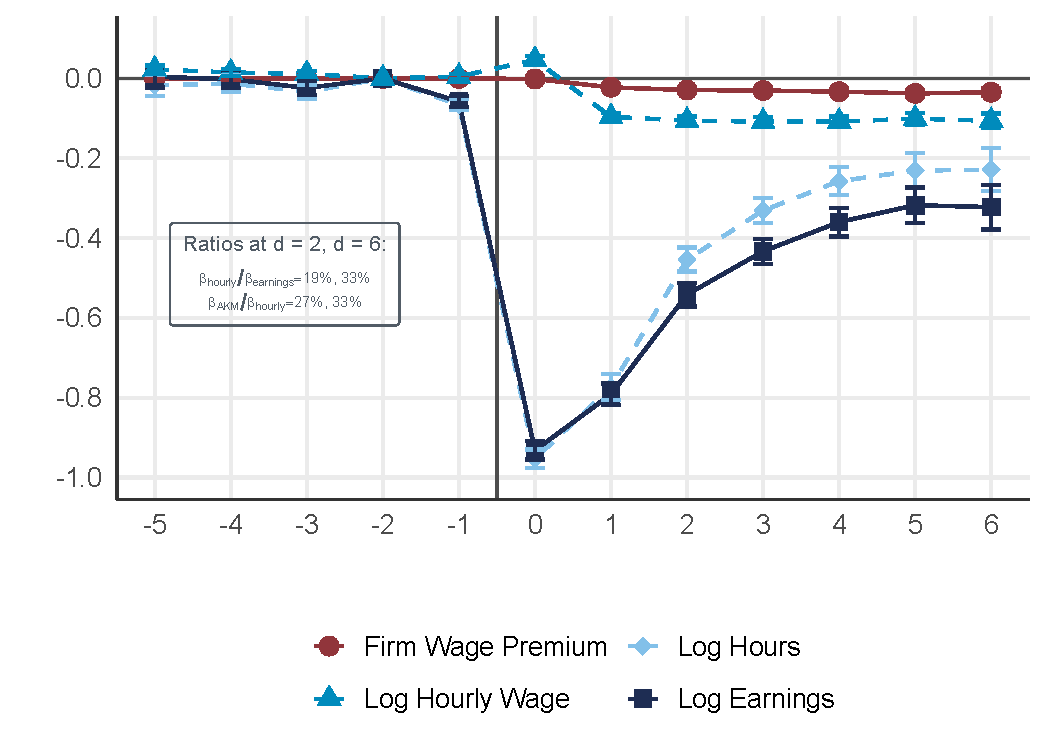
\includegraphics[width=\linewidth, trim={0cm 0cm 0.1cm 0cm}, clip,max width=\linewidth]{figures/01_event_figures/figure_1_le_wage_decomposition.pdf} \\
		\floatfoot{\footnotesize{\textsc{Notes}: This figure reports event-study estimates of the effect of job displacement on log hourly wage, log hours, log earnings and firm-specific wage premium for a sample of workers dismissed for economic reasons (LE)---see equation (\ref{eq:main_estimating_equation}) and associated text for more details on the specification. All estimates are computed on worker-years with positive hours and earnings, i.e.\ conditional on re-employment (see Section \ref{sec:decomposition_losses}). In the text, the ratios $\beta^{\text{AKM}}/\beta^{\text{earnings}}$ and $\beta^{\text{hourly}}/\beta^{\text{earnings}}$ are equal to the effect on firm-specific premium and hourly wage respectively divided by the effect on overall earnings and represents the fraction (expressed in percents) of total earnings losses due to each effect at $d=2,6$. \textbf{Sample}: The sample contains 8{,}341 individuals laid-off for economic reasons who end-up being re-employed post-displacement. \textbf{Outcomes}: Table \ref{apptab:definitions} provides more details on variables' definition.  Wage premia are estimated, following the AKM framework, as firm-fixed effects in a two-way regression of log-hourly wage on firm and worker fixed effects---see section \ref{sec:data:firm:premium} for more details. \textbf{Additional information}: Table \ref{tab:evstudytable_body} reports coefficients' value. Appendix Table \ref{apptab:evstudy_worker_outcomes} provides more details. \textbf{Standard errors}: robust standard errors clustered at the worker-level; displayed confidence intervals at the 99\% level.	}}
\end{center} \end{figure}


\begin{figure}[h!] \centering
	\caption{Productivity and labor share of current employers\label{fig:ln_apl_ls}}


	\begin{subfigure}[b]{.49\textwidth}
		\centering
		\caption[]{\small Productivity} \label{fig:prod_res_within_btw}
		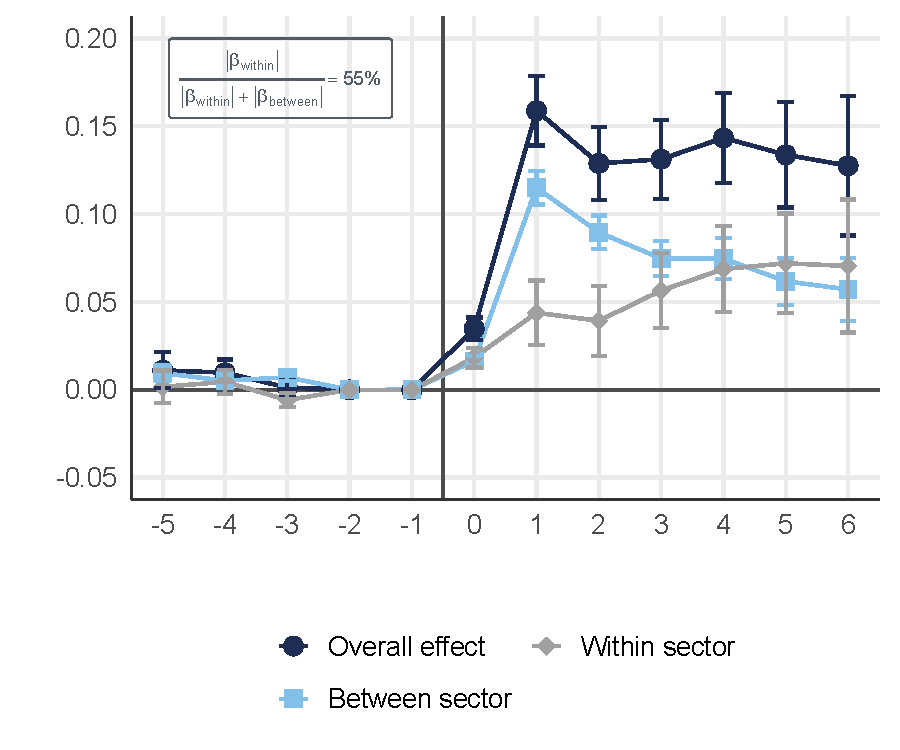
\includegraphics[scale=0.49,max width=\linewidth]{figures/01_event_figures/figure_2_a_productivity.pdf}
	\end{subfigure}
	\begin{subfigure}[b]{.49\textwidth}
		\centering
		\caption[]{\small Labor share of value-added} \label{fig:ln_Lshare_within_btw}
		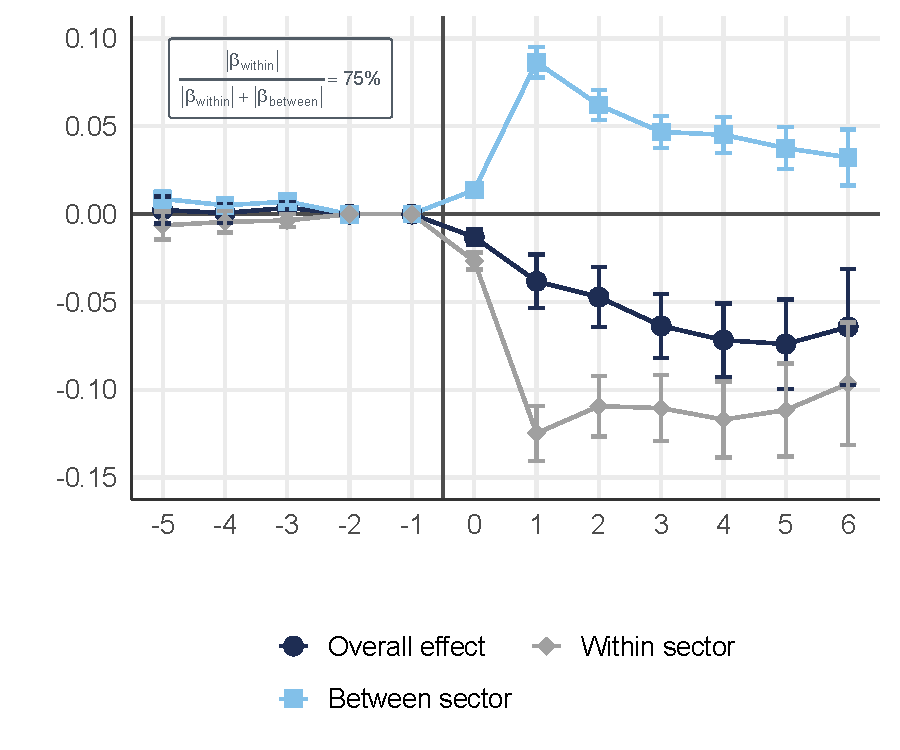
\includegraphics[scale=0.49,max width=\linewidth]{figures/01_event_figures/figure_2_b_labor_share.pdf}
	\end{subfigure}

	\begin{subfigure}[b]{.49\textwidth}
	\caption{Firm Wage Premium} \label{fig:firm_fe_within_btw}
	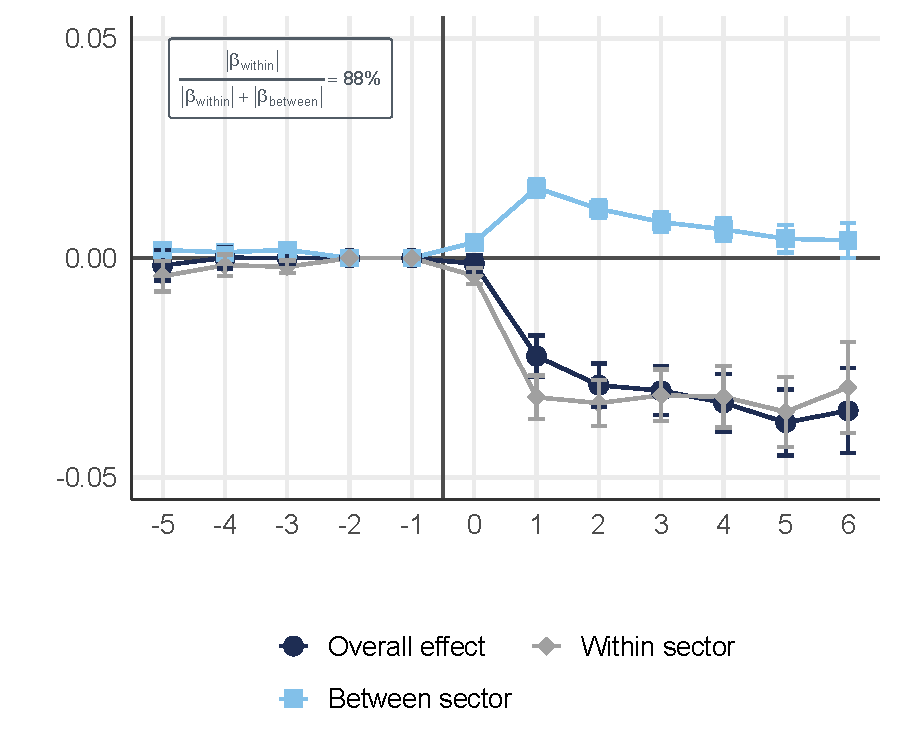
\includegraphics[width=\linewidth,max width=\linewidth]{figures/01_event_figures/figure_2_c_firm_premium.pdf}
	%	\floatfoot{\footnotesize{\textsc{Notes}: The sample contains 9,251 economic dismissals. 99\% confidence interval are displayed, based on robust standard errors clustered at the worker-level. The specification includes individual and year fixed-effects, see equation (\ref{eq:main_estimating_equation}) and associated text for more details. 
	%			Productivity is computed as the residual of a regression of value-added onto tangible capital and employment during the period 2001-2004.}}
\end{subfigure}


	\floatfoot{\footnotesize{\textsc{Notes}: 
			This figure reports event-study estimates of the effect of job displacement on the reallocation of workers towards firms with varying levels of productivity, value added per workers and labor share. Coefficients are obtained by estimating the specification of equation \ref{eq:main_estimating_equation} where the dependent variable is sequentially productivity, value added per worker and labor share. \textbf{Sample}: The sample contains 8,341 individuals laid-off for economic reasons who end-up being re-employed post-displacement. Productivty can be estimated for only 7,524 of those. \textbf{Comment on timing}: Firm-level outcomes are computed as three-year averages centered on $t^D-4$ (i.e.\ over $t^D-5$, $t^D-4$, and $t^D-3$), while displacements occur from 2005 to 2012. Accordingly, event-study coefficients reflect the movement of workers to firms with different initial characteristics and \textit{not} within-firm changes. \textbf{Definition of firm-level outcomes}: See Table \ref{apptab:definitions} for details. Productivity is the residual of an OLS regression of value-added on tangible capital and labor with year fixed effects. The labor share is computed as total labor cost over value-added. In lighter shade, we display the coefficients using a decomposition each of these variables as well as the AKM fixed-effect into a sectoral average at the 3-digit level (between sector $\bar{y}_s$ ) and a deviation from the sectoral average (within sector $R_i=y_i - \bar{y}_s$). The relative size of the within effect is computed as the absolute value of the within effect divided by the sum of the absolute value of the two effects, $|\beta_{\text{within}}| / (|\beta_{\text{within}}|+|\beta_{\text{between}}|)$, evaluated at the latest available horizon for each outcome: $t^D+5$ for productivity (where firm-level balance-sheet data are available only through that horizon) and $t^D+6$ for the labor share and the AKM firm wage premium. \textbf{Additional information}: Table \ref{tab:evstudytable_body} reports coefficients' value. Appendix Table \ref{apptab:evstudy_firm_outcomes} provides more details. \textbf{Standard errors}: robust standard errors clustered at the worker-level; displayed confidence intervals at the 99\% level.}}
\end{figure}

%, where value-added is deflated using 2-digit value added deflator (\textit{Indice de prix de la valeur ajoutée brute par branche})

%The sample contains 10,336 economic dismissals. 99\% confidence interval are displayed, based on robust standard errors clustered at the worker-level. The specification includes individual and year fixed-effects, see equation (\ref{eq:main_estimating_equation}) and associated text for more details. 

\begin{figure}[h!] \centering
	\caption{Quality of labor relations: firm-level measures  \label{fig:LE_accords}}
	%\caption{Firm-level collective agreements \label{fig:LE_accords}}
	\begin{subfigure}[b]{.49\textwidth}
		\centering
		\caption[]{\small Indicator of wage agreement (2005-2007)} \label{fig:LE_acc_main}
		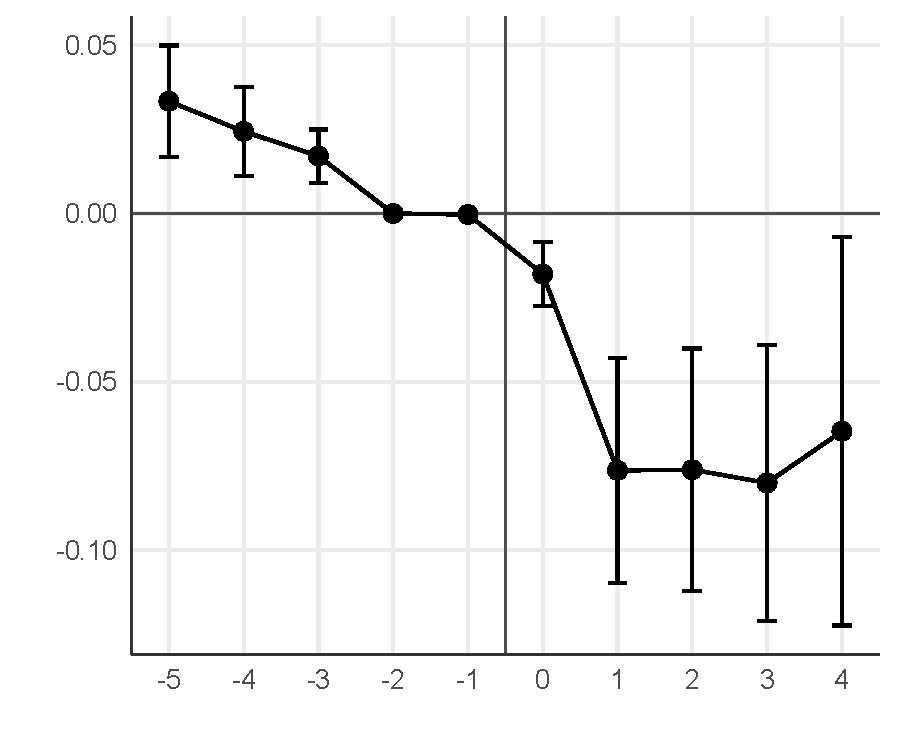
\includegraphics[width=\linewidth,max width=\linewidth]{figures/01_event_figures/figure_3_a_wage_agreement.pdf}
	\end{subfigure}
	\begin{subfigure}[b]{.49\textwidth}
		\centering
		\caption[]{\small Election turnout} \label{fig:LE_elec_main}
		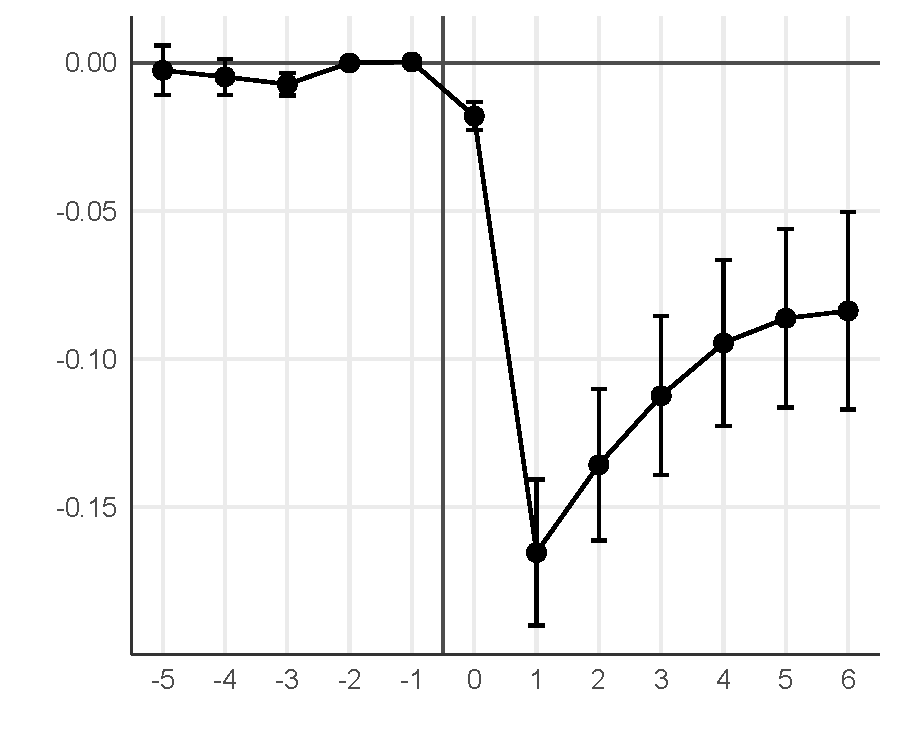
\includegraphics[width=\linewidth,max width=\linewidth]{figures/01_event_figures/figure_3_b_election_turnout.pdf}
	\end{subfigure}
	
	\floatfoot{\footnotesize{\textsc{Notes}: This figure reports event-study estimates of the effect of job displacement the reallocation of workers towards with varying propensities to conclude collective agreements (panel \ref{fig:LE_acc_main}) and turnouts at professional elections (panel \ref{fig:LE_elec_main})---see equation (\ref{eq:main_estimating_equation}) and associated text for more details on the specification. \textbf{Definition of the outcomes:} The dependent variable pertaining to collective agreements is an indicator equal to 1 when firms signed at least one agreement related to wages over the period 2005 to 2007. Because we restrict the focus to LE laid-off post 2007, we do not observe individuals after $t^D+4$. The variable on firm's average turnout at workplace election is computed based on elections taking place over 2009-2012. More details are provided in Section \ref{sec:Nego}, and Table \ref{apptab:definitions} provides more details on variables' definition. \textbf{Comment on timing:} Each firm is associated with a single value of each outcome, so that event-study coefficients reflect reallocation of workers between firms and not within-firm changes in such outcomes.
	\textbf{Additional information}: Appendix Tables \ref{tab:nego:LEnego_acc_result} and \ref{tab:nego:LEnego_ele_result} provide detailed results.
	\textbf{Standard errors}: robust standard errors clustered at the worker level; displayed confidence intervals at the 99\% level.}} 
\end{figure}



\FloatBarrier

%%%%%%%%%%%%%%%%%%%%%%%%%%%%%%%%%%%%%%%%%%%%%%%%%%%%%%%%%%%%%%%%%%
%%%%%%%%%%%%%%%%%%%%%%%%%%%%%%%%%%%%%%%%%%%%%%%%%%%%%%%%%%%%%%%%%%

\bibliographystyle{aer}
\bibliography{_REF}

%%%%%%%%%%%%%%%%%%%%%%%%%%%%%%%%%%%%%%%%%%%%%%%%%%%%%%%%%%%%%%%%%%
%%%%%%%%%%%%%%%%%%%%%%%%%%%%%%%%%%%%%%%%%%%%%%%%%%%%%%%%%%%%%%%%%%

\newpage
\appendix
%\appendixpage

\setcounter{page}{1}

\setcounter{table}{0}
\renewcommand{\thetable}{A\arabic{table}}

\setcounter{figure}{0}
\renewcommand{\thefigure}{A\arabic{figure}}

\begin{center}
	\noindent { \Large  {\textbf{Online Appendix to}: \\ \textbf{Understanding the Reallocation of Displaced Workers to Firms}}}\bigskip
	
	
	
	{\large
	Paul Brandily \qquad Camille Hémet \qquad Clément Malgouyres \qquad Patryk Wisniewski }\bigskip\\
	{\large April 2026}

\end{center}

\startcontents[sections]
\printcontents[sections]{l}{1}{\setcounter{tocdepth}{2}}

%%\begin{enumerate}
%%	\item[A] Additional Tables and Figures mentioned in the body of the paper
%%	\item[B] Details on the estimation procedure of the firm premiums 
%%	\item[A] Details on definition of the mass-layoff sample
%%    \item[A] Background information on labor market institutions in France 
%%\end{enumerate}


\clearpage
\section{Additional Tables and Figures}
%%%%%%%%%%%%%%%%%%%%%%%%%%%%%%%%%%%%%%%%%%%%%%%%%%%%%%%%%%%%%%%%%%%%%%%%%%%%%%%%%
%                                                                               %
% Cette version repart de 03_Draft\appendix\appendix_figures_tablesV1-short.tex %
%                                                                               %
%%%%%%%%%%%%%%%%%%%%%%%%%%%%%%%%%%%%%%%%%%%%%%%%%%%%%%%%%%%%%%%%%%%%%%%%%%%%%%%%%


\subsection{Figures}


\begin{figure}[h!] \centering
	\caption{LE Sample, baseline characteristics \label{fig:desc:LEquali}}
	\begin{subfigure}[b]{\textwidth}		
	\caption[]{\small Sector, NACE A10 (estimation sample vs.\ Panel DADS) \label{fig:desc:LEsec}}
		\centering
		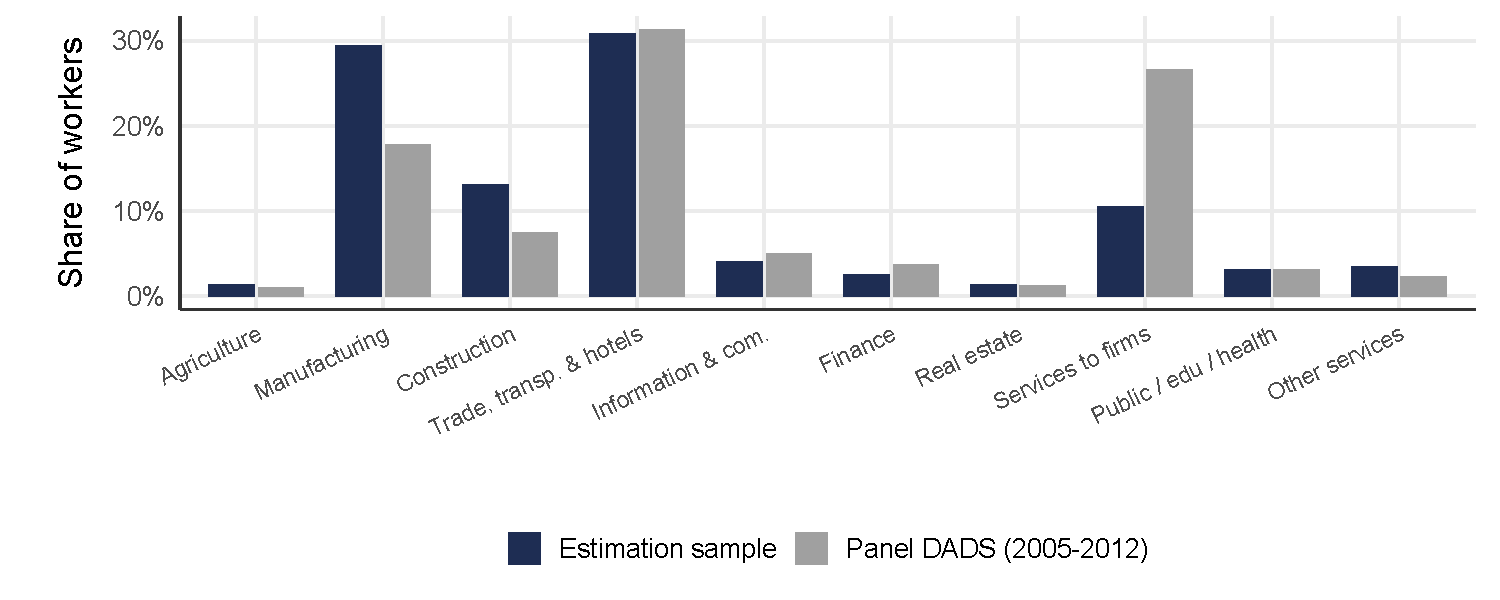
\includegraphics[width=0.69\linewidth, trim={0cm 0cm 0cm 0cm}, clip=true,max width=\linewidth]{figures/02_descriptive_figures/figure_A1_a_le_sectors.pdf}
	\end{subfigure}

	\begin{subfigure}[b]{\textwidth}
	\caption[]{\small Occupation \label{fig:desc:LEocc}}
		\centering
		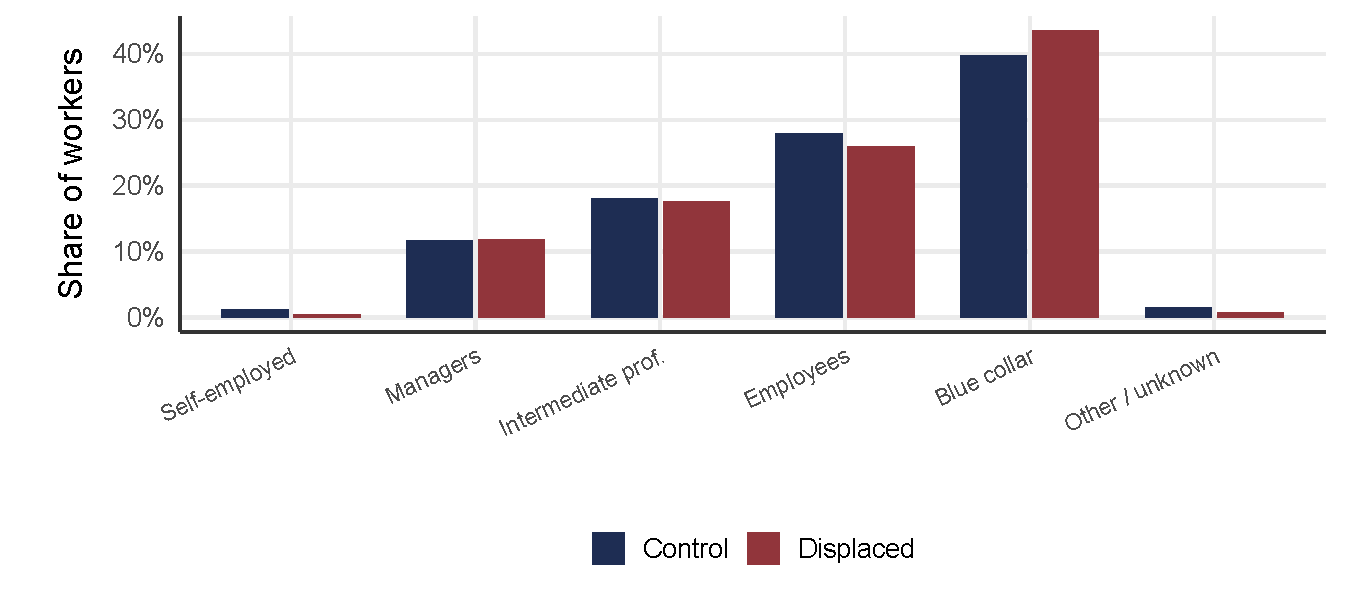
\includegraphics[scale=0.46, trim={0cm 0cm 0cm 0cm}, clip=true,max width=\linewidth]{figures/02_descriptive_figures/figure_A1_b_le_occupations.pdf}
	\end{subfigure}

	\begin{subfigure}[b]{\textwidth}
	\caption[]{\small Educational attainment \label{fig:desc:LEdip}}
		\centering
		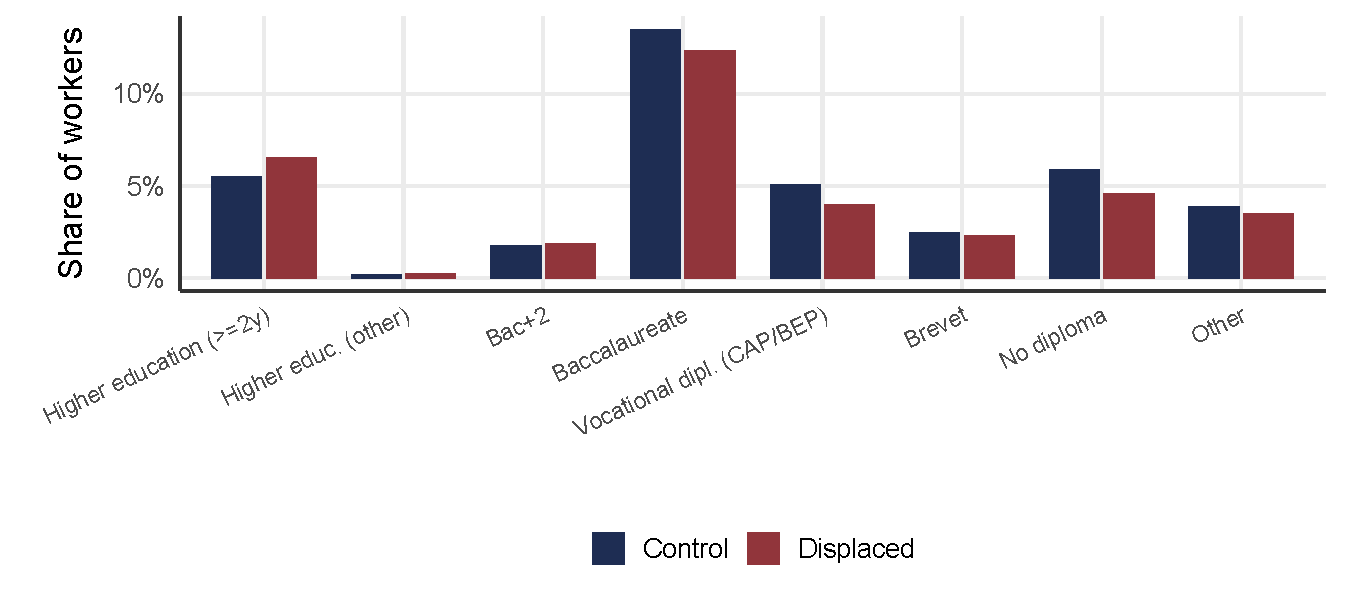
\includegraphics[scale=0.46, trim={0cm 0cm 0cm 0cm}, clip=true,max width=\linewidth]{figures/02_descriptive_figures/figure_A1_c_le_education.pdf}
	\end{subfigure}

	\floatfoot{\footnotesize{\textsc{Notes}: This figure presents descriptive statistics about the sample of 20,897 individuals displaced for economic reasons (LE) \textcolor{orange}{[21,132]} and their respective matched controls. Data is observed at $t^D-1$. Panel (a) reports the distribution of workers across NACE A10 sectors for our \emph{estimation sample} (controls only) and---for reference---the population of private-sector workers in the DADS panel over 2005--2012. We display the control group only because sector is a matching variable, so the LE-displaced and control-group distributions coincide at $t^D-1$ by construction; controls measured at $t^D-1$ are therefore an accurate description of the sectoral composition of the matched estimation sample. The third bar (Panel DADS) allows the reader to gauge how representative our estimation sample is of the broader French private-sector workforce. The ``Public / education / health'' bin (NAF~84--88) does not include employees of the central administration as our DADS sample covers only private-law contracts, so workers in this bin are employed under private-law contracts in para-public organizations such as \emph{établissements publics à caractère industriel et commercial} (EPIC), the social-security system, and private clinics, schools, and social-work non-profits operating in publicly-funded sectors. Panels (b) and (c) display the distribution of workers across occupations and educational attainment. Educational attainment is only observed for a sub-sample. These two variables were not used in the matching algorithm. In both cases, the sample appears to be balanced across treatment and controls.}}
\end{figure}


\begin{figure}[h!] \centering
	\caption{Displacement Effects in Level: Earnings, Employment and Hours} \label{fig:aveffect_emp_earn}
	%\begin{subfigure}[b]{.6\textwidth}
	%\centering
	%\caption[]{\small LE: Wage Losses} \label{fig:event_sbr}
	%\includegraphics[scale=0.3,max width=\linewidth]{03_Draft/graphs/event_sbr}
	%\end{subfigure}
	%%        \vskip
	\begin{subfigure}[b]{.49\textwidth}
		\centering
		\caption[]{\small Annual Earnings (in level) \label{fig:event_sbr}} 	
		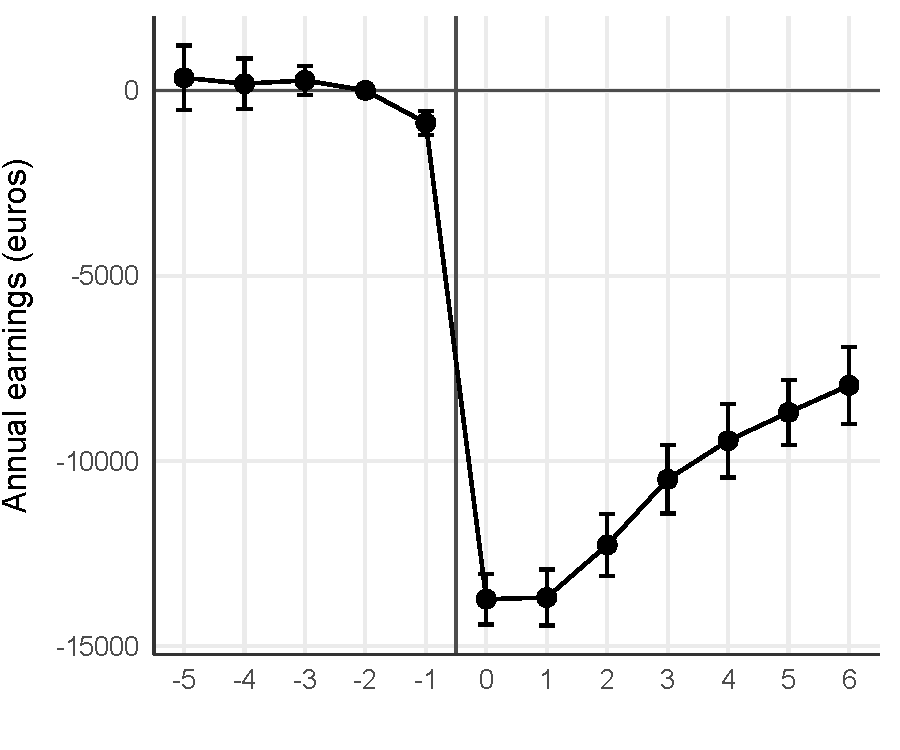
\includegraphics[scale=0.49,max width=\linewidth]{figures/01_event_figures/figure_A2_a_earnings.pdf}
	\end{subfigure}
	\begin{subfigure}[b]{.49\textwidth}
		\centering
		\caption[]{\small Employment Probability \label{fig:event_emp}} 
		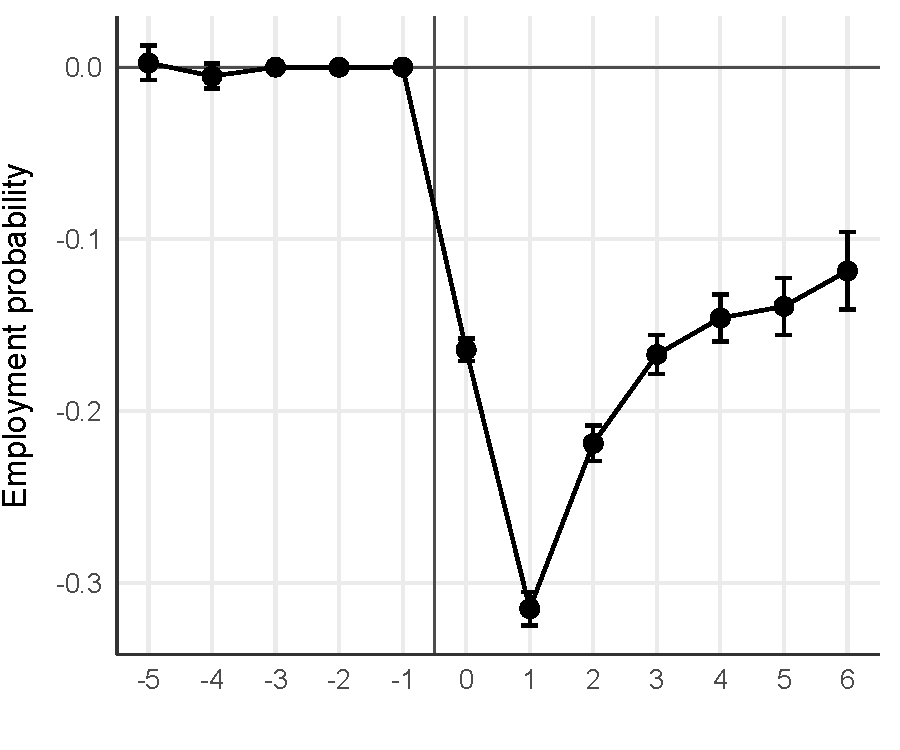
\includegraphics[scale=0.49,max width=\linewidth]{figures/01_event_figures/figure_A2_b_employment.pdf}
	\end{subfigure}
	%\vskip
	\begin{subfigure}[b]{.49\textwidth}
		\centering
		\caption[]{\small Hours Worked  \label{fig:event_hours}} 
		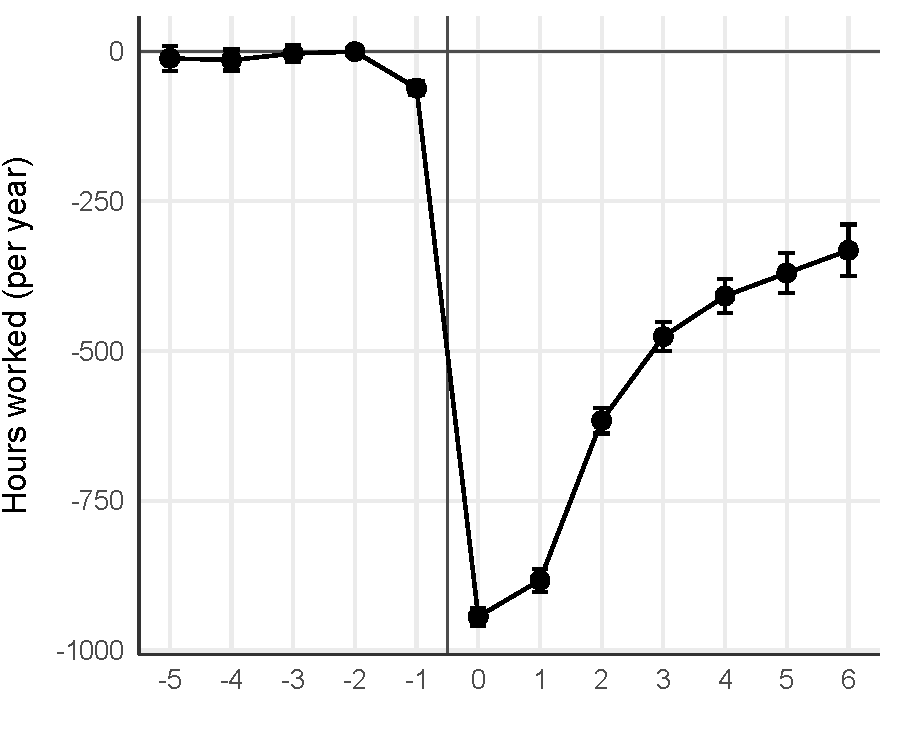
\includegraphics[scale=0.49,max width=\linewidth]{figures/01_event_figures/figure_A2_c_hours.pdf}
	\end{subfigure}
	%\begin{subfigure}[b]{.49\textwidth}
	%	\centering
	%	\caption[]{\small Hourly Wage \label{fig:event_hwr}} 
	%	\includegraphics[scale=0.49,max width=\linewidth]{figures-2026/event_lnsbrhour_Log.pdf}
	%\end{subfigure}
	
	\floatfoot{\footnotesize{\textsc{Notes}: This figure reports event-study estimates of the cost of job displacement for a sample of workers dismissed for economic reasons (LE) ---see equation (\ref{eq:main_estimating_equation}) and associated text for more details on the specification. \textbf{Samples}: The sample contains 20{,}897 individuals laid-off for economic reasons and their matched controls. All three panels use the full estimation sample; non-employed workers are assigned earnings and hours of zero. \textbf{Definition of the outcomes:} Table \ref{apptab:definitions} summarizes variables' definition. \textbf{Additional information}: Appendix Table \ref{apptab:evstudy_worker_outcomes} provides more details. For brevity, effect on hours is only displayed when using log. \textbf{Standard errors}: robust standard errors clustered at the worker-level; displayed confidence intervals at the 99\% level. }}
\end{figure}


\begin{figure}[h!]\caption{Wage decomposition on the LE sample restricted to firms with at least 10 employees}
\label{fig:wage_decomposition_size10}
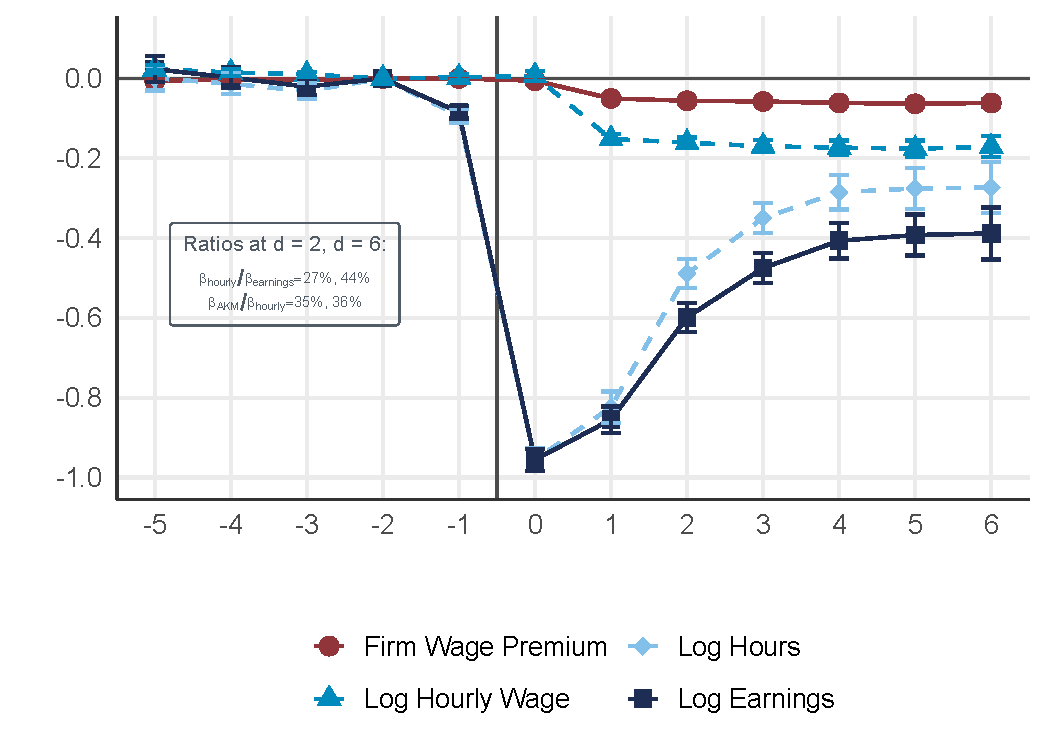
\includegraphics[width=\linewidth, trim={0cm 0cm 0.1cm 0cm}, clip,max width=\linewidth]{figures/01_event_figures/figure_A3_le_size10_wage_decomposition.pdf}
\par\medskip
\floatfoot{\footnotesize\textsc{Notes}: This figure reproduces Figure~\ref{fig:fe_current_event} of the paper (wage decomposition for the LE sample) on the subset of workers displaced from firms with at least $10$ employees prior to the event. Coefficients and ratios are very close to the baseline reported in Figure~\ref{fig:fe_current_event}, indicating that the patterns we document are not driven by displacements from very small firms.}
\end{figure}


\begin{figure}[h!]\caption{Wage decomposition on the LE sample, with unrestricted AKM (no exclusion of LE/MLO trajectories)}\label{fig:paper_R_wage_decomposition_god2}
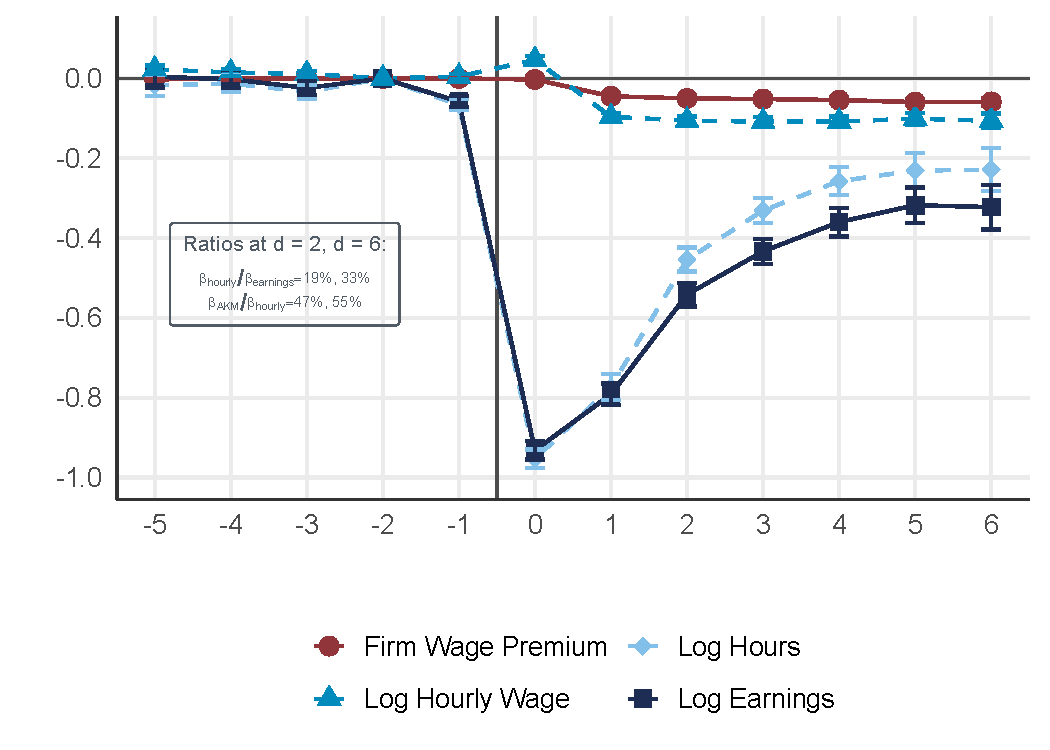
\includegraphics[width=\linewidth, trim={0cm 0cm 0.1cm 0cm}, clip,max width=\linewidth]{figures/01_event_figures/figure_A4_le_unrestricted_akm.pdf}
\par\medskip
\floatfoot{\footnotesize\textsc{Notes}: This figure reports the wage decomposition for the LE sample, using the unrestricted AKM, which does not exclude any worker, i.e. without correcting for contamination. Compared to the results in Figure~\ref{fig:fe_current_event}, the share of the hourly-wage scar attributable to the firm premium drop is larger by about $15$--$20$ percentage points under the unrestricted AKM at all post-displacement horizons. The difference reflects the bias introduced by displaced workers' post-layoff wage trajectories on the firm fixed effects of firing firms.
}
\end{figure}


% Added in the R2 revision (Referee 3, point 3): robustness of the premium loss to the AKM estimation window.
\begin{figure}[h!]\caption{Loss in firm wage premium by AKM estimation window (LE sample)}\label{fig:akm_windows}
\centering
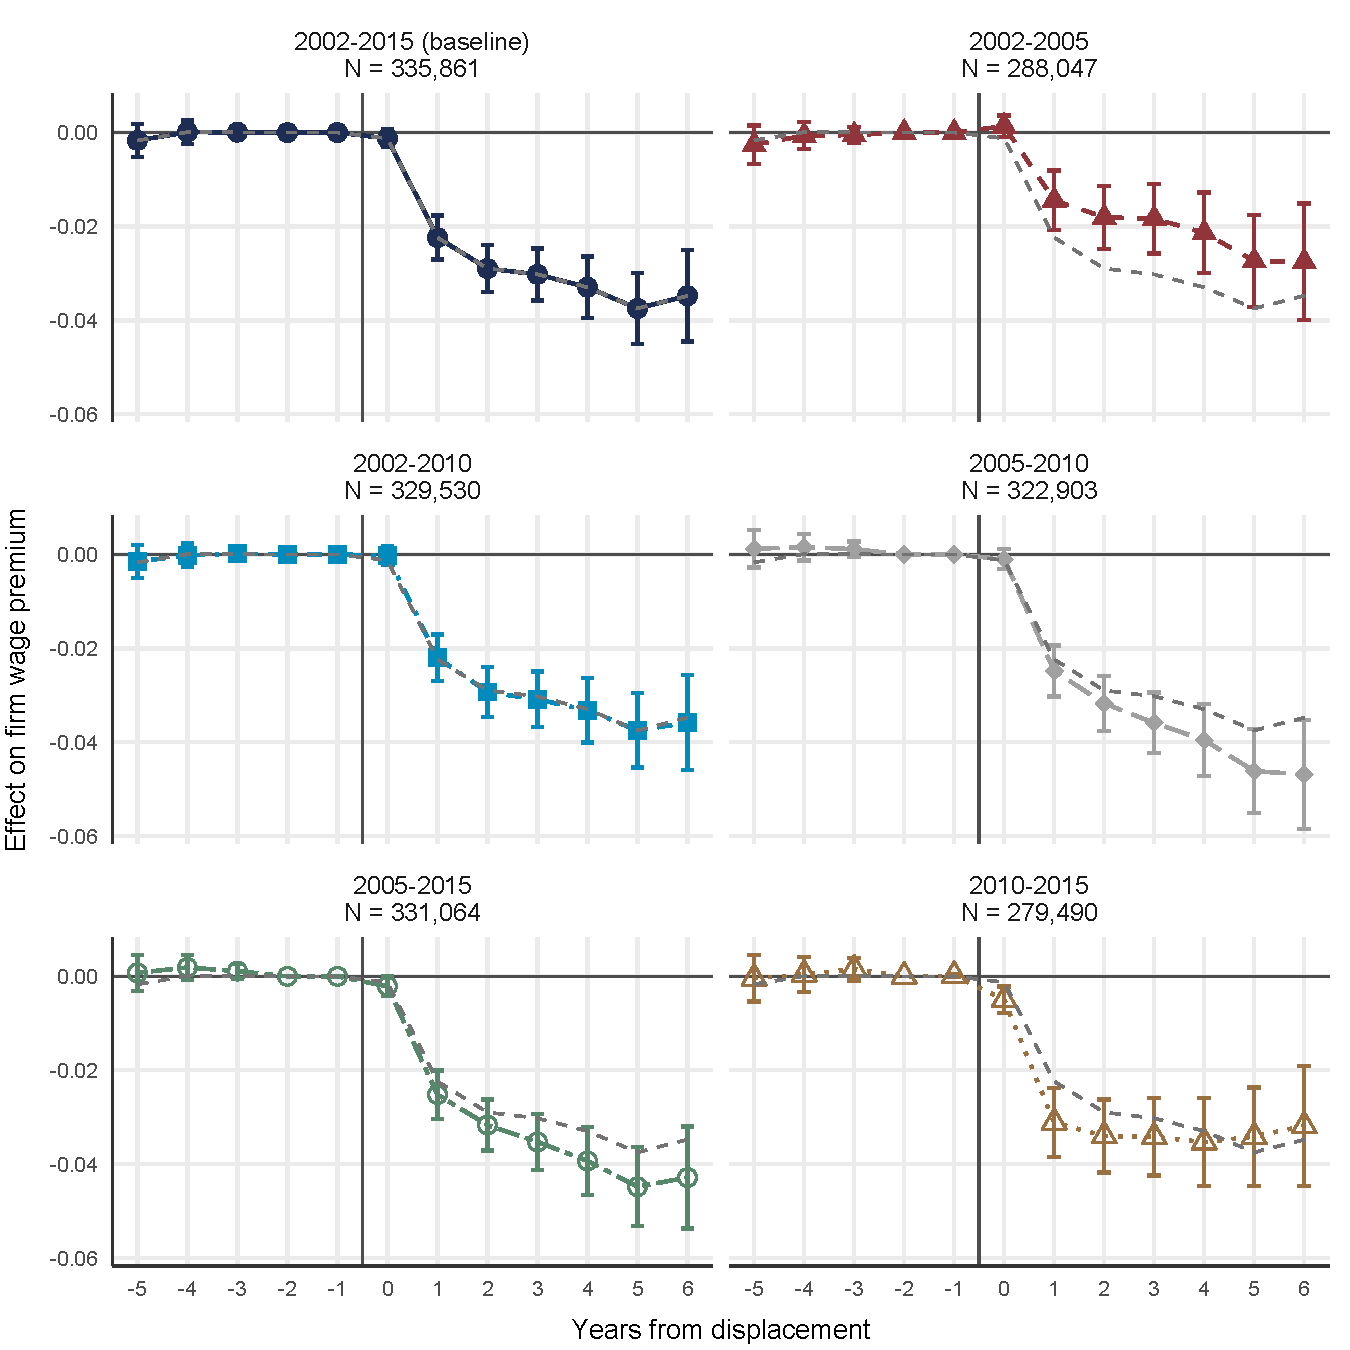
\includegraphics[width=0.95\linewidth,height=0.7\textheight,keepaspectratio]{figures/03_akm_periods/figure_A5_akm_estimation_windows.pdf}
\par\medskip
\floatfoot{\footnotesize\textsc{Notes}: Event-study estimates of the effect of job displacement on the firm wage premium of the current employer (equation \ref{eq:main_estimating_equation}), for the LE sample. In each panel, the AKM firm fixed effects are estimated over the window indicated in the title; the top-left panel (2002--2015) is the baseline of Figure \ref{fig:fe_current_event}, and is reproduced as a dashed grey line in the other panels. $N$ is the number of worker-year observations; it varies across windows because the set of firms with an estimated premium changes with the window. $t^D-2$ is the reference period. Standard errors are clustered at the worker level.}
\end{figure}


\begin{figure}[h!] \begin{center}
		\caption{Decomposition of the cost of job displacement: Mass-layoff (MLO) sample} \label{fig:fe_current_event_mlo_pretrends}
		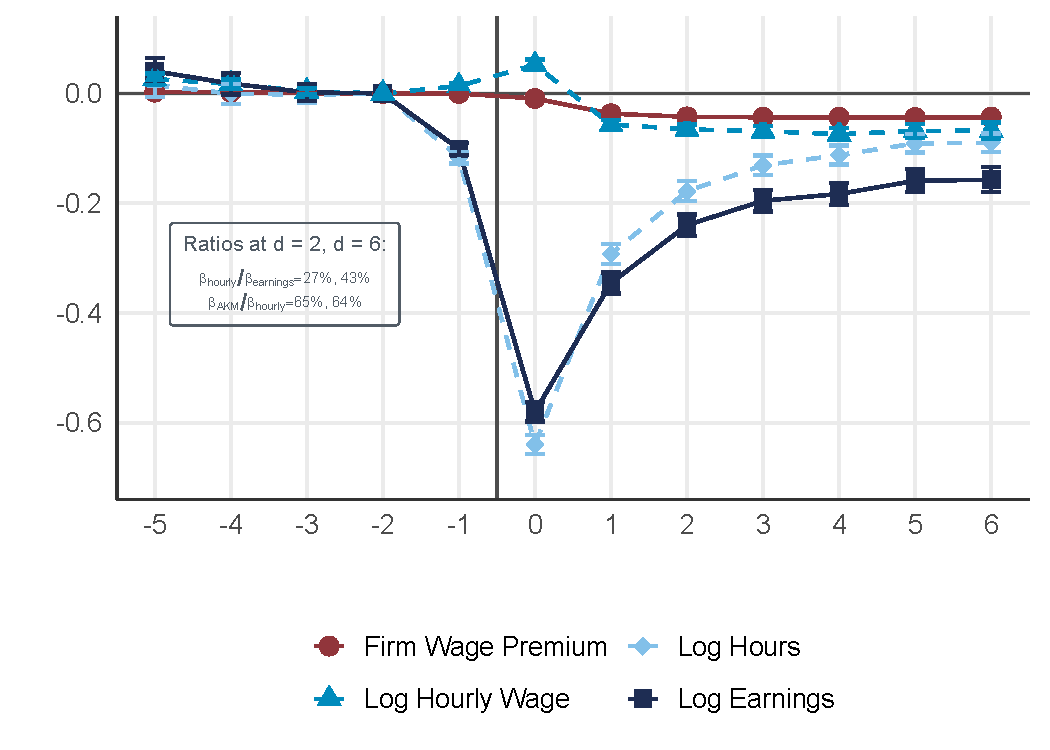
\includegraphics[width=\linewidth, trim={0cm 0cm 0.1cm 0cm}, clip,max width=\linewidth]{figures/01_event_figures/figure_A6_mlo_baseline_wage_decomposition.pdf} \\
		\floatfoot{\footnotesize{\textsc{Notes}: This figure reports event-study estimates of the effect of job displacement on log hourly wage, log hours, log earnings and firm-specific wage premium for a sample of workers displaced in a mass layoff (MLO30). It is the analogue of Figure~\ref{fig:fe_current_event} for the MLO30 sample---see equation (\ref{eq:main_estimating_equation}) and associated text for more details on the specification. \textbf{Sample}: The sample contains 17,949 individuals displaced in a mass layoff \textcolor{orange}{[17,946]} and as many controls; the regressions on log hourly wage and firm wage premium are restricted to person-distance cells with non-missing post-displacement hourly wage. Details on the construction of the sample are provided in Appendix~\ref{appsec:mlo_details}. \textbf{Outcomes}: Table~\ref{apptab:definitions} summarizes variables' definition. Wage premia are estimated, following the AKM framework, as firm-fixed effects in a two-way regression of log-hourly wage on firm and worker fixed effects---see Section~\ref{sec:data:firm:premium} for more details. \textbf{Additional information}: Table~\ref{apptab:evstudy_worker_outcomes_mlo} provides more details. \textbf{Standard errors}: robust standard errors clustered at the worker-level; displayed confidence intervals at the 99\% level.}}

\end{center} \end{figure}




\begin{figure}[h!] \centering
	\caption{Productivity, labor share and firm wage premium of current employers, MLO sample \label{fig:prod_et_al_MLO}}
	\begin{subfigure}[b]{.49\textwidth}
		\centering
		\caption[]{\small Productivity} \label{fig:prod_res_mlo}
		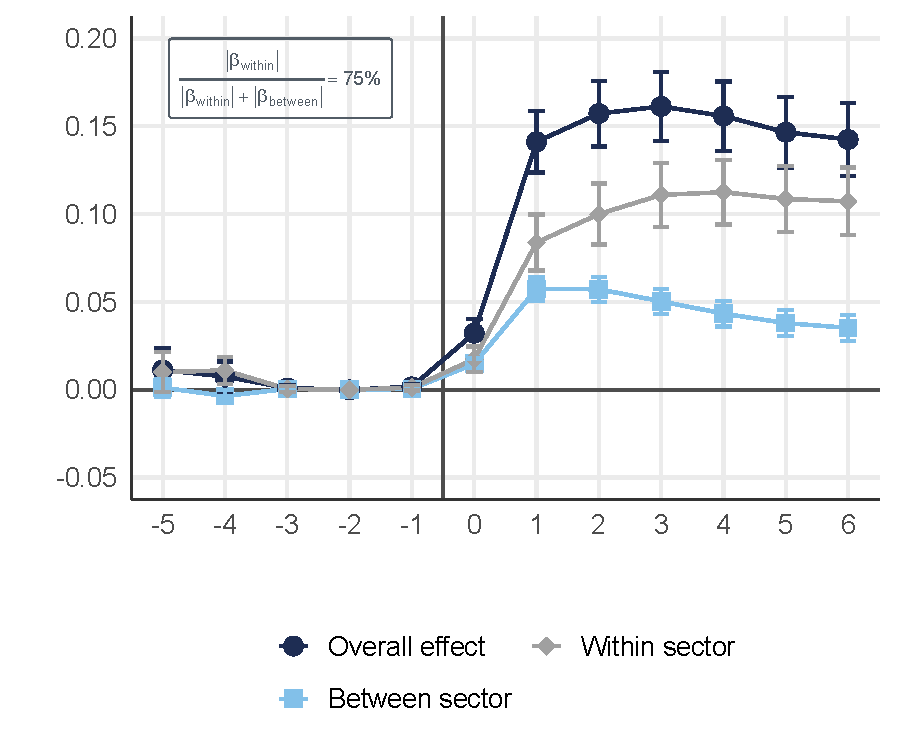
\includegraphics[scale=0.49,max width=\linewidth]{figures/01_event_figures/figure_A7_a_baseline_productivity.pdf}
	\end{subfigure}
	\begin{subfigure}[b]{.49\textwidth}
		\centering
		\caption[]{\small Labor share of value-added} \label{fig:ln_Lshare_mlo}
		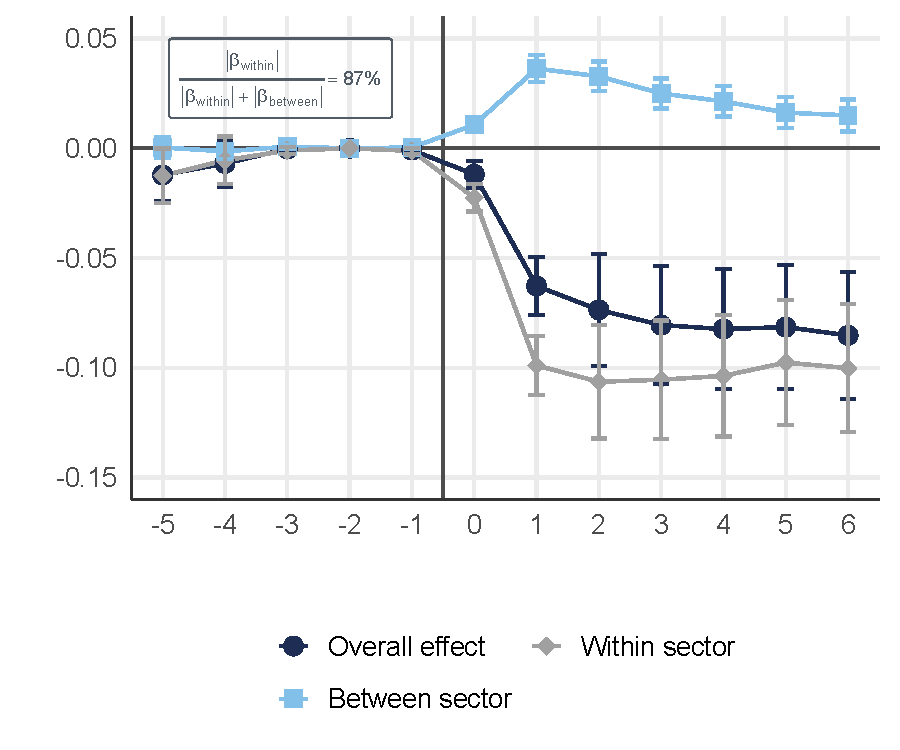
\includegraphics[scale=0.49,max width=\linewidth]{figures/01_event_figures/figure_A7_b_baseline_labor_share.pdf}
	\end{subfigure}

	\begin{subfigure}[b]{.49\textwidth}
		\caption{Firm Wage Premium} \label{fig:firm_fe_mlo}
		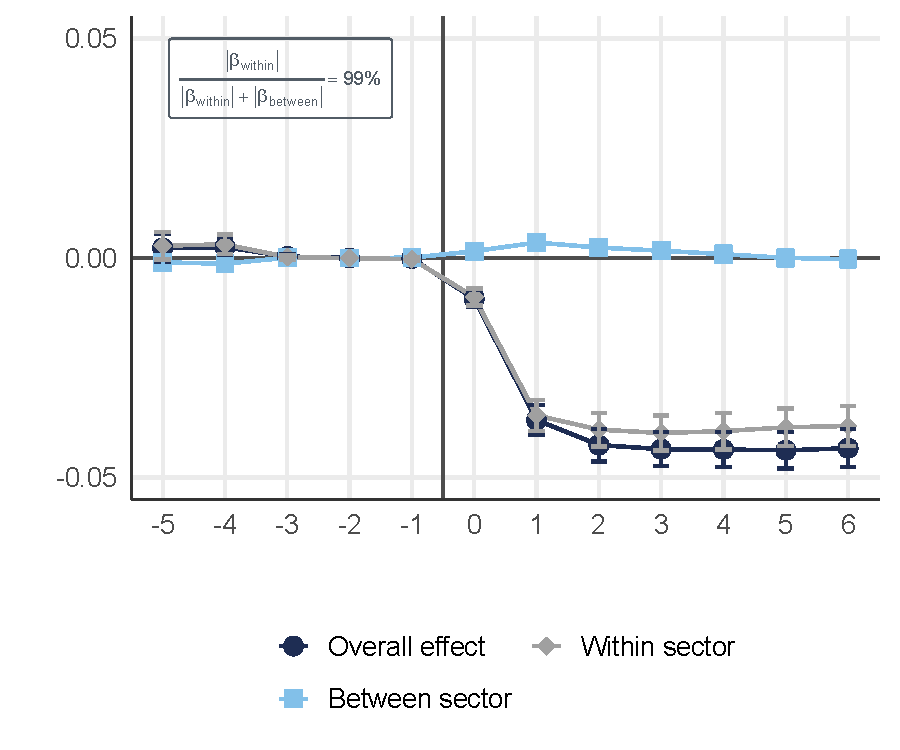
\includegraphics[width=\linewidth,max width=\linewidth]{figures/01_event_figures/figure_A7_c_baseline_firm_premium.pdf}
	\end{subfigure}

	\floatfoot{\footnotesize{\textsc{Notes}: This figure reports event-study estimates of the effect of job displacement on the reallocation of workers towards firms with varying levels of productivity, labor share, and AKM firm wage premium, for the MLO30 sample. It is the analogue of Figure~\ref{fig:ln_apl_ls} for workers displaced in a mass layoff. Coefficients are obtained by estimating the specification of equation \ref{eq:main_estimating_equation} where the dependent variable is sequentially productivity, labor share, and firm wage premium. \textbf{Sample}: The sample contains 17,949 individuals displaced in a mass layoff \textcolor{orange}{[17,946]} (MLO30) and as many controls; the regressions condition on re-employment in a private-sector firm with non-missing firm characteristics. \textbf{Comment on timing}: Firm-level outcomes (productivity, labor share) are computed as three-year averages centered on $t^D-4$ (i.e.\ over $t^D-5$, $t^D-4$, and $t^D-3$), while displacements occur from 2005 to 2012. Accordingly, event-study coefficients reflect the movement of workers to firms with different initial characteristics and \textit{not} within-firm changes. \textbf{Definition of firm-level outcomes}: See Table \ref{apptab:definitions} for details. Productivity is the residual of an OLS regression of value-added on tangible capital and labor with year fixed effects. The labor share is computed as total labor cost over value-added. Wage premia are estimated, following the AKM framework, as firm-fixed effects in a two-way regression of log-hourly wage on firm and worker fixed effects---see section \ref{sec:data:firm:premium} for more details. In lighter shade, we display the coefficients using a decomposition of each of these variables into a sectoral average at the 3-digit level (between sector $\bar{y}_s$) and a deviation from the sectoral average (within sector $R_i = y_i - \bar{y}_s$). \textbf{Additional information}: Appendix Table \ref{apptab:evstudy_firm_outcomes_mlo} provides more details. \textbf{Standard errors}: robust standard errors clustered at the worker-level; displayed confidence intervals at the 99\% level.}}
		
		
		
		

\end{figure}



\FloatBarrier

\begin{figure}[h!]
\centering
\caption{Wage decomposition by sex (LE sample)\label{fig:fe_current_event_by_sex}}

\begin{subfigure}[b]{\textwidth}
\centering
\caption*{\small (a) Men}
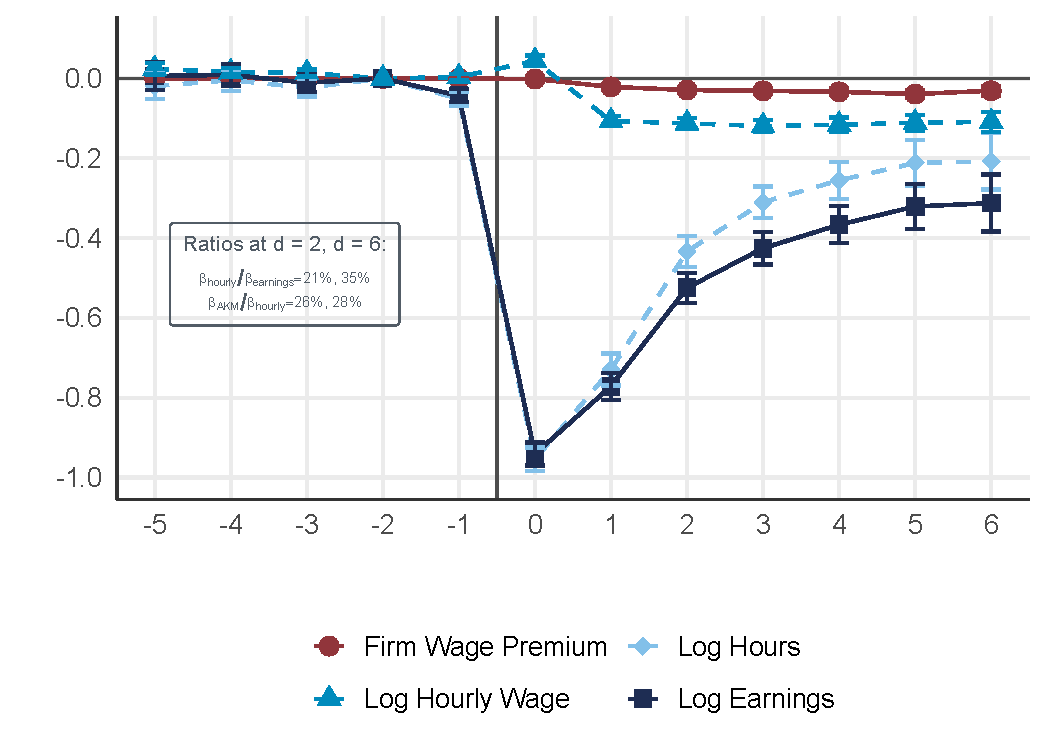
\includegraphics[width=0.75\linewidth, trim={0cm 0cm 0.1cm 0cm}, clip,max width=\linewidth]{figures/01_event_figures/figure_A8_a_men.pdf}
\end{subfigure}

\medskip

\begin{subfigure}[b]{\textwidth}
\centering
\caption*{\small (b) Women}
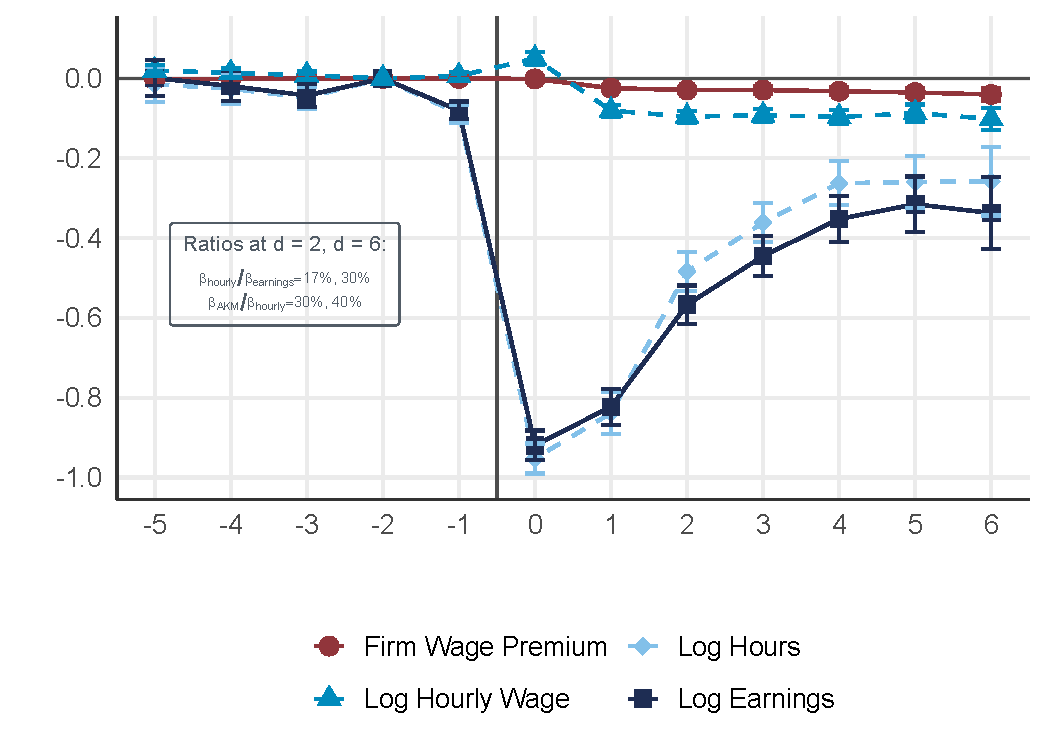
\includegraphics[width=0.75\linewidth, trim={0cm 0cm 0.1cm 0cm}, clip,max width=\linewidth]{figures/01_event_figures/figure_A8_b_women.pdf}
\end{subfigure}

\floatfoot{\footnotesize{\textsc{Notes}: This figure reproduces Figure~\ref{fig:fe_current_event} of the paper for men and women separately, on the LE sample. Men and women display similar profiles on the four outcomes: the hourly-wage scar at $t^D+5$ is $-0.105$ for men against $-0.089$ for women, and the AKM firm-premium scar is $-0.041$ for men against $-0.045$ for women. The hours and total-earnings scars are slightly larger for men than for women. \textbf{Sample}: $n_{\text{men}} = $ men, $n_{\text{women}} = $ women in the LE sample. \textbf{Standard errors}: robust standard errors clustered at the worker level; displayed confidence intervals at the $99\%$ level.}}
\end{figure}

\FloatBarrier

\begin{figure}[h!]
	\caption{Firms characteristics over the full period 2002--2015, LE sample \label{fig:prod_et_al_Full_LE}}
	\centering
	\begin{subfigure}[b]{.49\textwidth}
		\centering
		\caption[]{\small Productivity}
		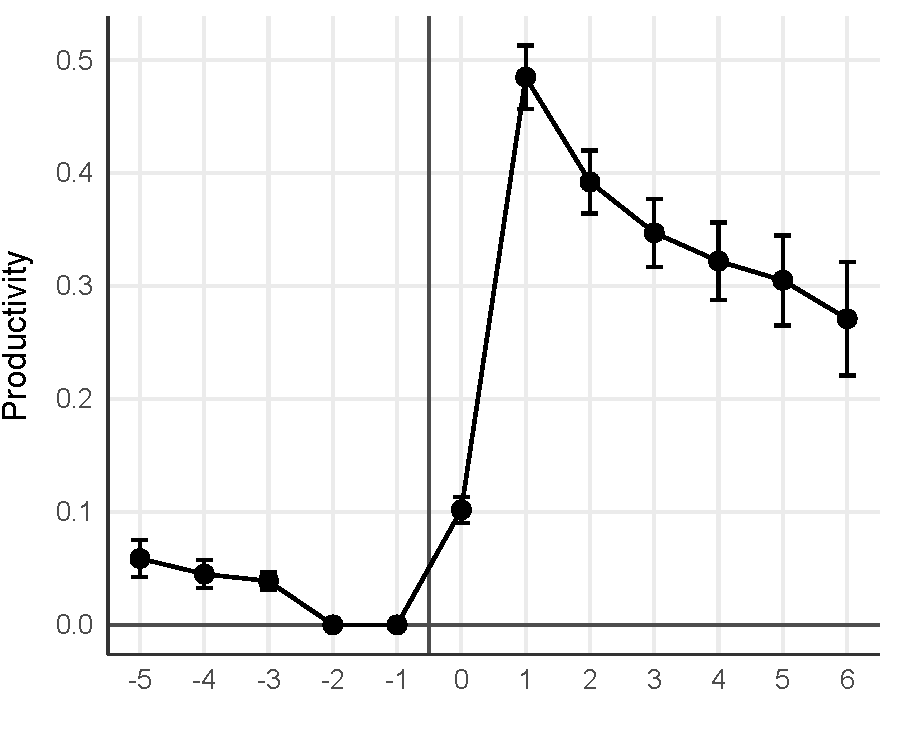
\includegraphics[scale=0.49,max width=\linewidth]{figures/01_event_figures/figure_A9_a_productivity.pdf}
	\end{subfigure}
	\begin{subfigure}[b]{.49\textwidth}
		\centering
		\caption[]{\small Log of value-added per worker}
		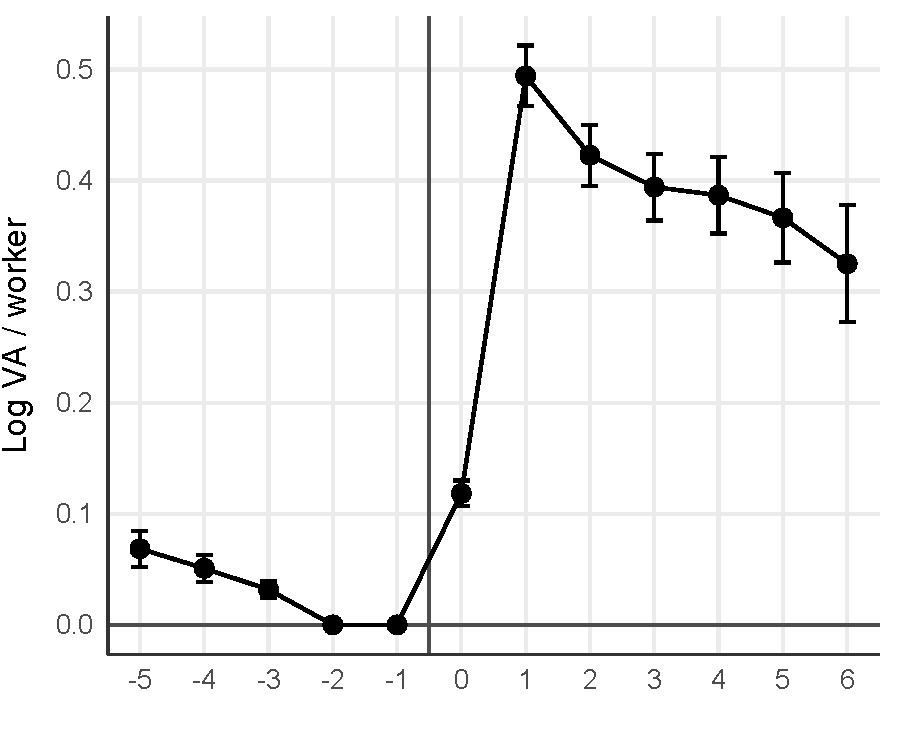
\includegraphics[scale=0.49,max width=\linewidth]{figures/01_event_figures/figure_A9_b_va_per_worker.pdf}
	\end{subfigure}
	\begin{subfigure}[b]{.49\textwidth}
		\centering
		\caption[]{\small Log of labor share of value-added}
		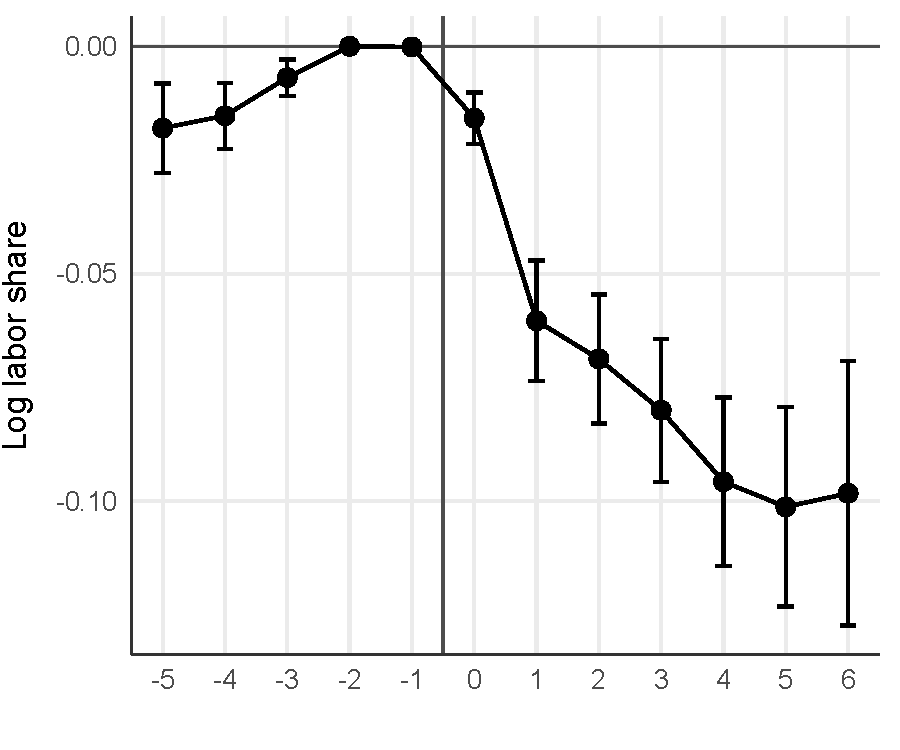
\includegraphics[scale=0.49,max width=\linewidth]{figures/01_event_figures/figure_A9_c_labor_share.pdf}
	\end{subfigure}
	\floatfoot{\footnotesize{\textsc{Notes}: This figure reports event-study estimates of the effect of job displacement on the reallocation of workers towards firms with varying levels of productivity, value added per workers and labor share. Coefficients are obtained by estimating the specification of equation \ref{eq:main_estimating_equation} where the dependent variable is sequentially productivity, value added per worker and labor share. \textbf{Sample}: The sample contains 8,341 individuals laid-off for economic reasons who end-up being re-employed post-displacement. Productivty can be estimated for only 7,524 of those. \textbf{Comment on timing}: Firm-level outcomes are computed as the average of the firm-level outcome over the full period 2002--2015, while displacements occurs at $t^D$ (with $t^D$ between 2005 and 2012). Accordingly, event-study coefficients reflect the movement of displaced workers to firms with different time-invariant characteristics and \textit{not} changes within-firm in such characteristics. \textbf{Definition of firm-level outcomes}: Table \ref{apptab:definitions} summarizes variables' definition. Value added per worker is computed as value added over reported employment. Productivity is obtained as the residual of an OLS regression of value-added on the book value of tangible capital and labor with year fixed effects. The labor share is computed as total labor cost over value-added, averaged over 2002--2015.  \textbf{Standard errors}: robust standard errors clustered at the worker-level; displayed confidence intervals at the 99\% level.}}
\end{figure}



\begin{figure*}[h!]
	\caption{Firms characteristics over the full period 2002--2015, MLO sample \label{fig:prod_et_al_Full_MLO}}
	\centering
	\begin{subfigure}[b]{.49\textwidth}
		\centering
		\caption[]{\small Productivity}
		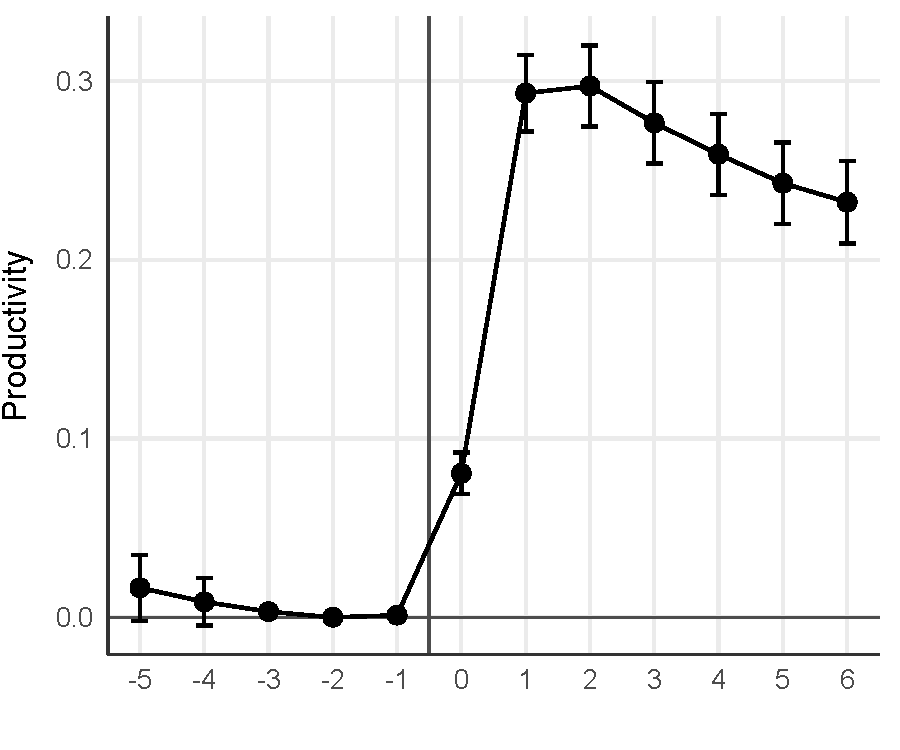
\includegraphics[scale=0.49,max width=\linewidth]{figures/01_event_figures/figure_A10_a_productivity.pdf}
	\end{subfigure}
	\begin{subfigure}[b]{.49\textwidth}
		\centering
		\caption[]{\small Log of value-added per worker}
		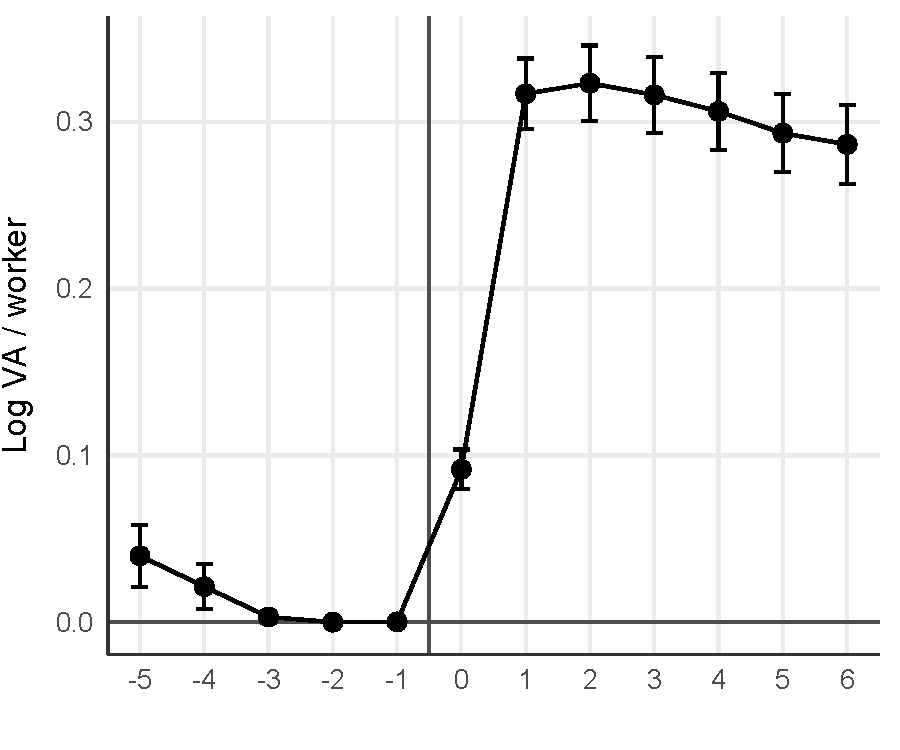
\includegraphics[scale=0.49,max width=\linewidth]{figures/01_event_figures/figure_A10_b_va_per_worker.pdf}
	\end{subfigure}
	\begin{subfigure}[b]{.49\textwidth}
		\centering
		\caption[]{\small Log of labor share of value-added}
		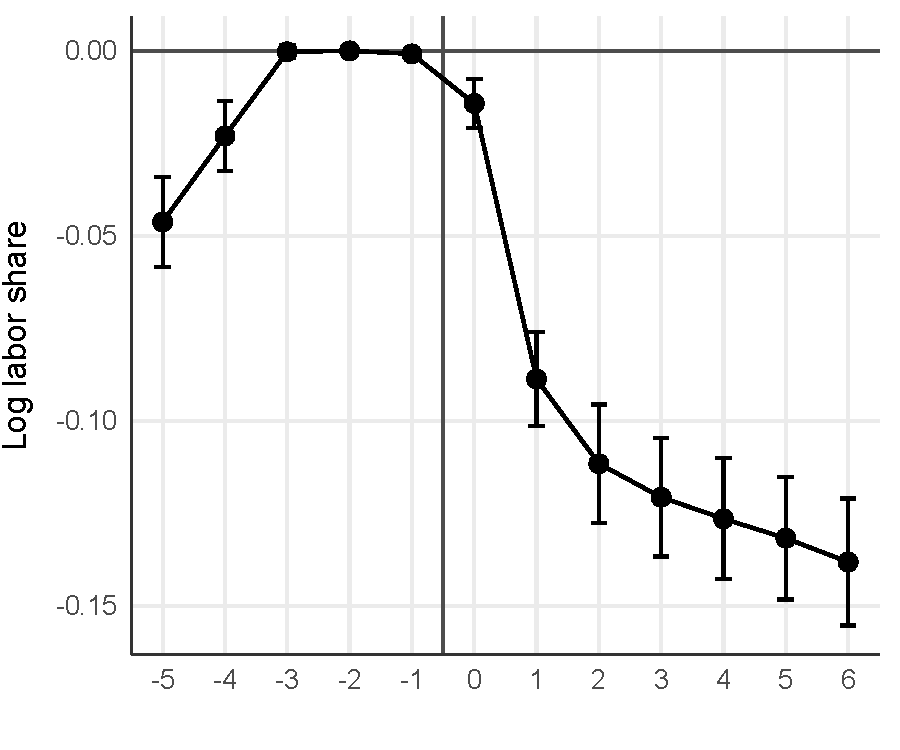
\includegraphics[scale=0.49,max width=\linewidth]{figures/01_event_figures/figure_A10_c_labor_share.pdf}
	\end{subfigure}
	\floatfoot{\footnotesize{\textsc{Notes}: This figure reports event-study estimates of the effect of job displacement on the reallocation of workers towards firms with varying levels of productivity, value added per workers and labor share. Coefficients are obtained by estimating the specification of equation \ref{eq:main_estimating_equation} where the dependent variable is sequentially productivity, value added per worker and labor share. \textbf{Sample}: The sample contains 4,772 individuals laid-off for economic reasons who end-up being re-employed post-displacement. Productivty can be estimated for only 4,130 of those. \textbf{Comment on timing}: Firm-level outcomes are computed as the average of the firm-level outcome over the full period 2002--2015, while displacements occurs at $t^D$ (with $t^D$ between 2005 and 2012). Accordingly, event-study coefficients reflect the movement of displaced workers to firms with different time-invariant characteristics and \textit{not} changes within-firm in such characteristics. \textbf{Definition of firm-level outcomes}: Table \ref{apptab:definitions} summarizes variables' definition. Value added per worker is computed as value added over reported employment. Productivity is obtained as the residual of an OLS regression of value-added on the book value of tangible capital and labor with year fixed effects. The labor share is computed as total labor cost over value-added, averaged over 2002--2015.  \textbf{Standard errors}: robust standard errors clustered at the worker-level; displayed confidence intervals at the 99\% level.}}
\end{figure*}



\begin{figure}[h!]
	\caption{Firm-level event-study of laying-off firms' productivity, LE sample \label{fig:firm_es_productivity}}
	\centering
	\begin{subfigure}[b]{.49\textwidth}
		\centering
		\caption[]{\small Residual productivity}
		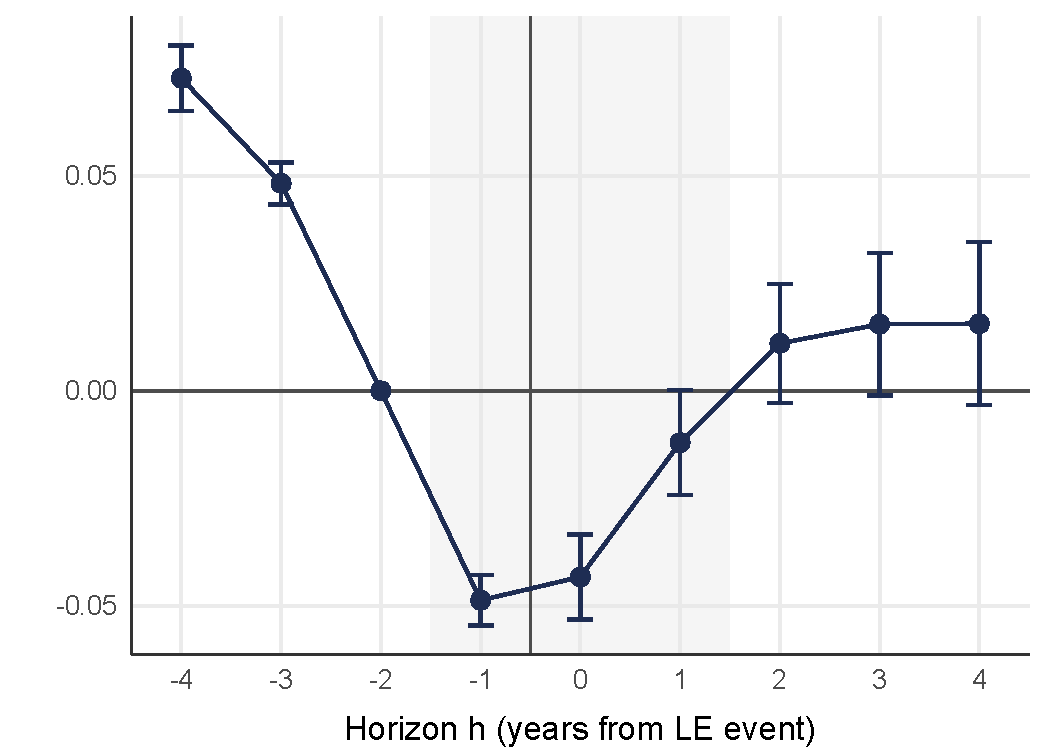
\includegraphics[scale=0.49,max width=\linewidth]{figures/01_event_figures/figure_A11_a_layoff_firm_productivity.pdf}
	\end{subfigure}
	\begin{subfigure}[b]{.49\textwidth}
		\centering
		\caption[]{\small TFP (Cobb--Douglas)}
		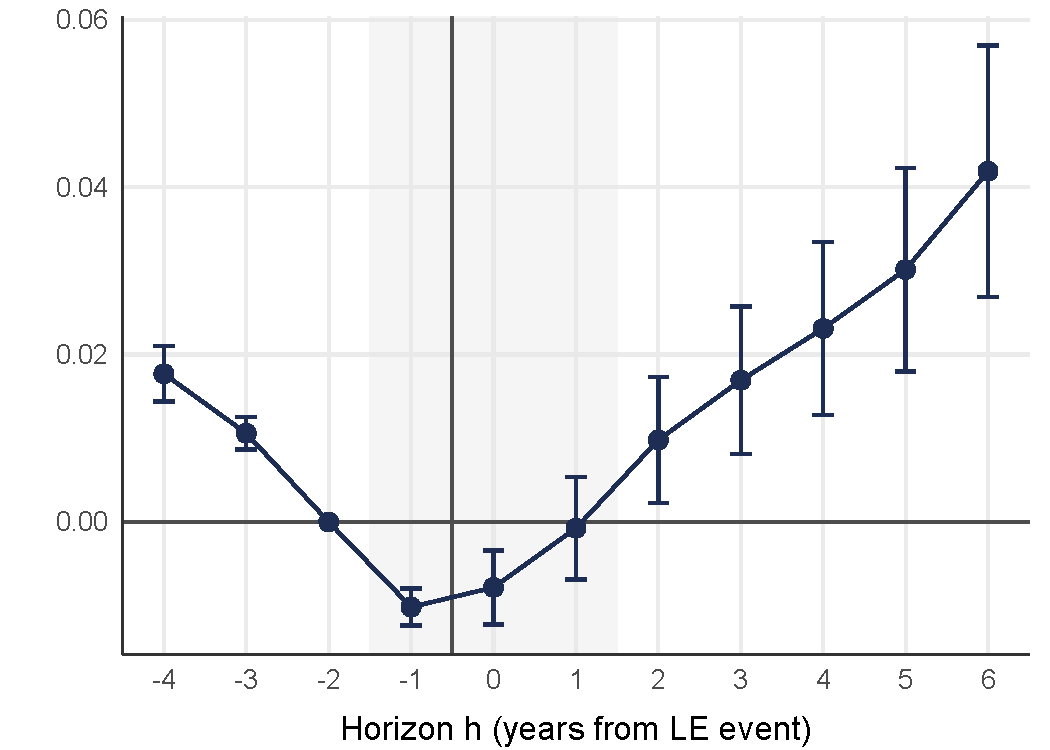
\includegraphics[scale=0.49,max width=\linewidth]{figures/01_event_figures/figure_A11_b_layoff_firm_tfp.pdf}
	\end{subfigure}
	% \begin{subfigure}[b]{.49\textwidth}
	% 	\centering
	% 	\caption[]{\small TFP (translog)}
	% 	\includegraphics[scale=0.49,max width=\linewidth]{figures-2026/firm_es_tfp_tl.pdf}
	% \end{subfigure}
	\floatfoot{\footnotesize{\textsc{Notes}: This figure reports event-study estimates from a firm-level event study where the unit of observation is the firm (\textit{not the worker}). Treated firms ($n=8{,}001$) are firms experiencing their first economic-layoff event between 2005 and 2012 (LE sample); the omitted reference horizon is $h=-2$. The dependent variables are 3-year moving averages of firm-level productivity centered on year $t$, i.e.\ averaged over $[t-1, t, t+1]$. Horizons $h \in \{-1, 0, +1\}$ (shaded) overlap with the layoff year and should be interpreted as a transition window; horizons $h \geq +2$ are the first windows containing only post-layoff years. Panel (a) plots the results for the residual of an OLS regression of value-added on tangible capital and labor with year fixed effects; panel (b) plots the results for Cobb--Douglas TFP estimates, imposing common factor coefficients across firms within 2-digit sectors. Standard errors are clustered at the firm level; displayed confidence intervals are at the 99\% level.}}
\end{figure}



\begin{figure}[h!] \centering
	\caption{Firm-specific wage premium and productivity \label{fig:bscatter_firmfe_prod}}
	\begin{subfigure}[b]{.49\textwidth}
		\centering
		\caption[]{\small Value-added per worker} \label{fig:firm_LE_binscatter_ln_apl}
		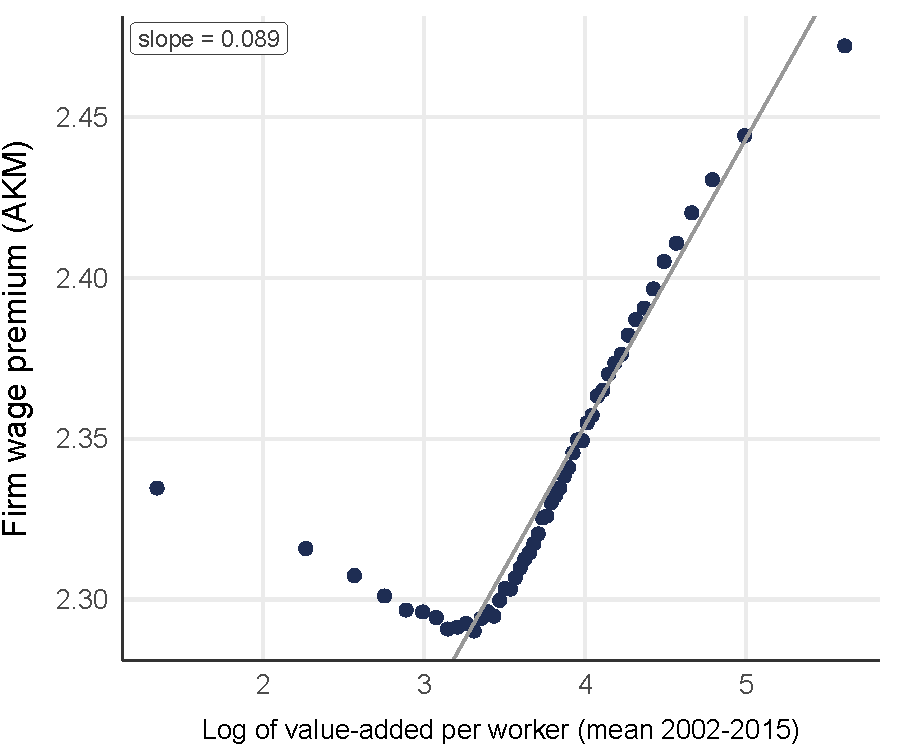
\includegraphics[scale=0.49,max width=\linewidth]{figures/02_descriptive_figures/figure_A12_a_va_per_worker.pdf}
	\end{subfigure}
	\begin{subfigure}[b]{.49\textwidth}
		\centering
		\caption[]{\small Productivity} \label{fig:firm_LE_binscatter_prod_res}
		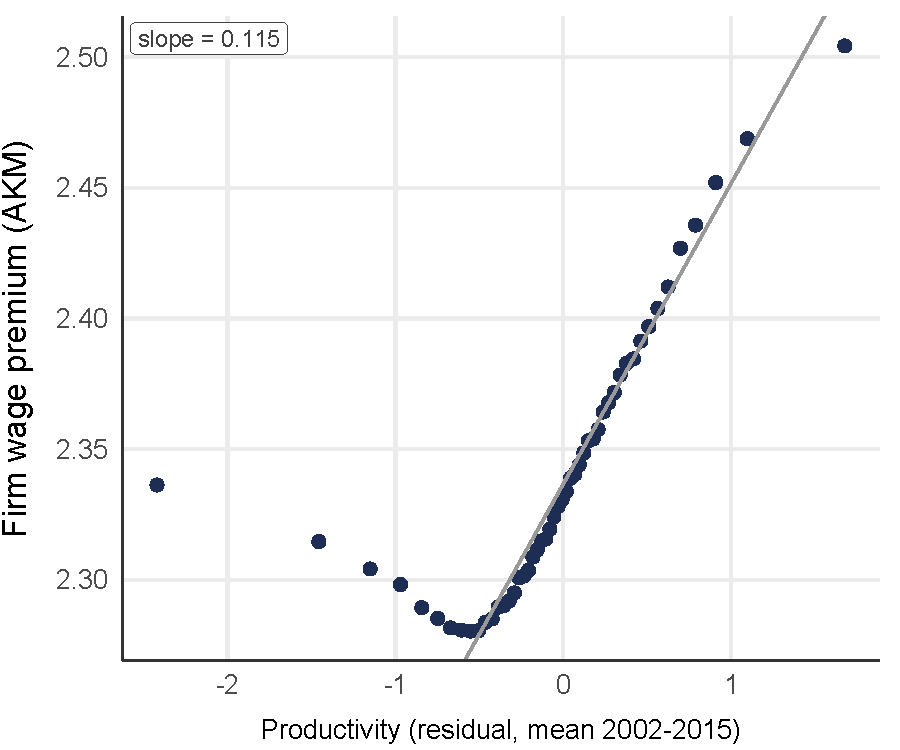
\includegraphics[scale=0.49,max width=\linewidth]{figures/02_descriptive_figures/figure_A12_b_productivity.pdf}
	\end{subfigure}
	
	\floatfoot{\footnotesize{\textsc{Notes}: This figure displays the binned scatter plot of firm-premia with respect to (log) value-added per worker (left panel) and productivity (right panel). 50 quantiles are used. The linear fit (light gray line) is estimated on a sample excluding the bottom 5 and the top 1 quantiles. As in the Portuguese data \citep[][see in particular Figure IV, page 663]{card2016bargaining}, the firm AKM fixed-effects and value-added per worker (or productivity) are strongly positively associated outside of the bottom of the distribution.  Fitted slope=0.085 (left) and 0.095 (right). \textcolor{orange}{[0.089 and 0.115, as printed on the R2 figure]} \textbf{Definition of variables}: Table \ref{apptab:definitions} summarizes variables' definition. Value-added per worker is computed as value-added over reported employment. Productivity is obtained as the residual of an OLS regression of value-added on the book value of tangible capital and labor with year fixed effects, where value-added is deflated using 2-digit value added deflator (\textit{Indice de prix de la valeur ajoutée brute par branche}). }} 
\end{figure}


\begin{figure}[h!] \centering
	\caption{Firm-specific wage premium and bargaining outcomes\label{fig:bscatter_firmfe_bargaining}}
	\begin{subfigure}[b]{.49\textwidth}
		\centering
		\caption[]{\small Indicator of wage agreement} \label{fig:firm_LE_binscatter_wage_agreement}
		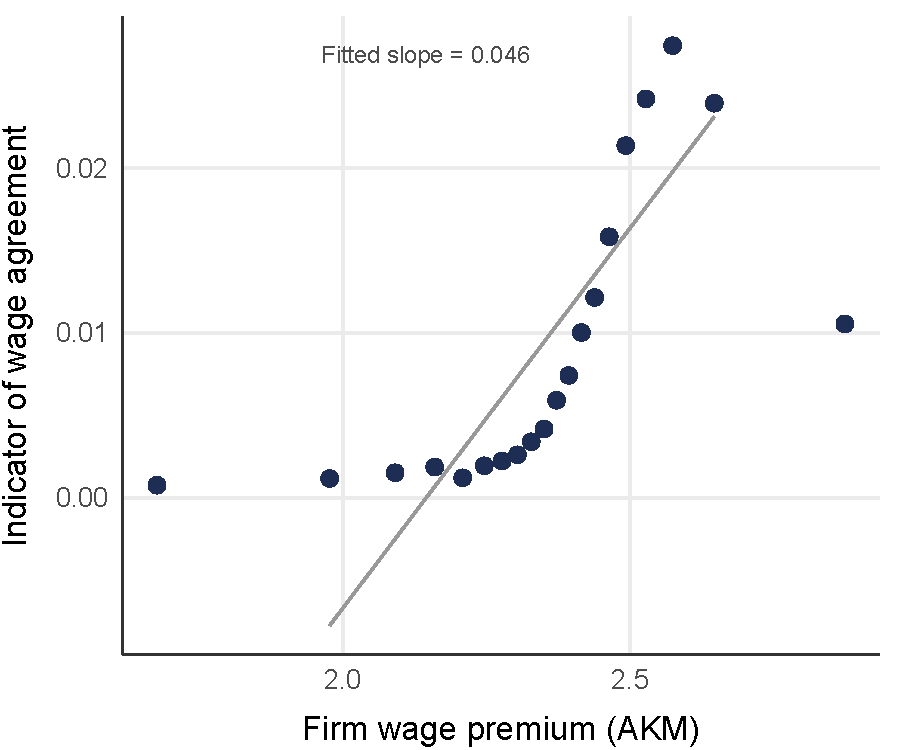
\includegraphics[scale=0.49,max width=\linewidth]{figures/02_descriptive_figures/figure_A13_a_wage_agreement.pdf}
	\end{subfigure}
	\begin{subfigure}[b]{.49\textwidth}
		\centering
		\caption[]{\small Election turnout} \label{fig:firm_LE_binscatter_election_turnout}
		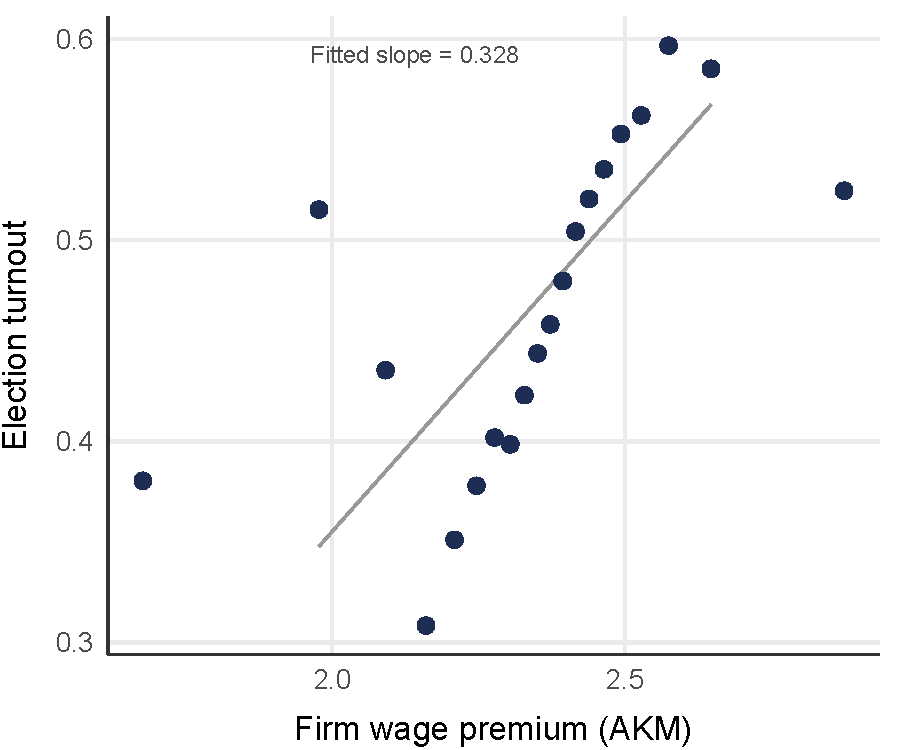
\includegraphics[scale=0.49,max width=\linewidth]{figures/02_descriptive_figures/figure_A13_b_election_turnout.pdf}
	\end{subfigure}

	\floatfoot{\footnotesize{\textsc{Notes}: This figure complements Figure~\ref{fig:bscatter_firmfe_prod} by showing the binned scatter plot of two firm-level bargaining outcomes against the firm-specific AKM premium $\widehat\psi_f$ (contamination-corrected): an indicator of wage-agreement signing over 2005--2007 (panel a) and the firm-level average turnout at 2009--2012 workplace elections (panel b). Firms are grouped into 20 quantiles of $\widehat\psi_f$. Linear fits (light gray) are estimated excluding the bottom and top quantile bins. Both bargaining outcomes are strongly positively associated with the firm wage premium (fitted slopes: $0.586$ for wage agreement, $0.298$ for election turnout) \textcolor{orange}{[0.046 and 0.328, as printed on the R2 figure; with 0.046 the agreement indicator is no longer ``strongly'' associated with the premium---reword]}, suggesting that worker bargaining power is one of the firm-level dimensions captured by the AKM premium. \textbf{Definition of variables}: see Table~\ref{apptab:definitions} for full definitions; the wage-agreement indicator equals one if the firm signed at least one wage-related agreement over 2005--2007, and election turnout is the firm-level average turnout at 2009--2012 workplace elections.}}
\end{figure}

\begin{figure}[h!] \centering
	\caption{Distribution of firm fixed effects in the sample of displaced workers: comparison with previous work \label{fig:sample_FEdist}}
		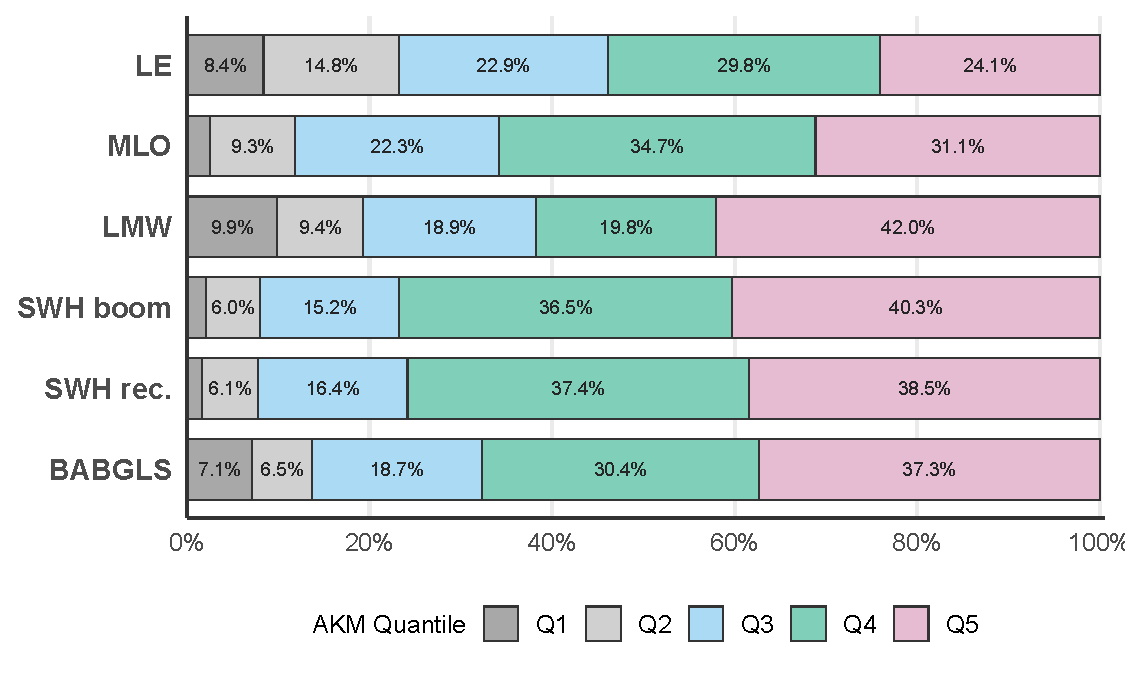
\includegraphics[width=\linewidth,max width=\linewidth]{figures/02_descriptive_figures/figure_A14_firm_premium_distribution.pdf}
	
	\floatfoot{\footnotesize{\textsc{Notes}: This figure displays the distribution of the firm AKM fixed-effects in the estimating sample. It presents the share of observations falling into each of the five quintiles of the AKM distribution (computed on the population of firms) for our economic-layoff sample (LE) and our mass-layoff sample (MLO30). For comparison we also report the corresponding figures from related papers in the displacement literature: LMW \citep{Lachowska2020}; SWH \citep{Schmieder2020}, for which we distinguish boom and recession episodes; and BABGLS \citep{bertheau_etal_2023}. In the first row (LE), 55.9\% of displaced workers come from firms in the top two quintiles \textcolor{orange}{[53.9\%, as printed on the R2 figure]} of the AKM premium distribution---above the 40\% benchmark a fully representative sample would deliver, indicating moderate over-representation of high-premium firms. The MLO row is more skewed: the corresponding share is 67.7\% \textcolor{orange}{[65.8\%]}, consistent with the fact that mass-layoff events tend to occur disproportionately in larger and higher-premium firms. The four remaining rows put these numbers in perspective: in all comparable papers, the share of displaced workers in the top two quintiles is at least as high as in our MLO sample (61.8\% in LMW, 75.9--76.8\% in SWH boom and recession, 67.7\% in BABGLS), and our LE sample is the least skewed of all six. The over-representation of high-premium firms is therefore noticeably milder in our LE design than in the rest of the literature.}}
\end{figure}



\begin{figure}[h!] 
	\caption{Raw Means on Earnings in Control and Treatment Groups\label{fig:raw_mean_earnings}} 
	\centering
	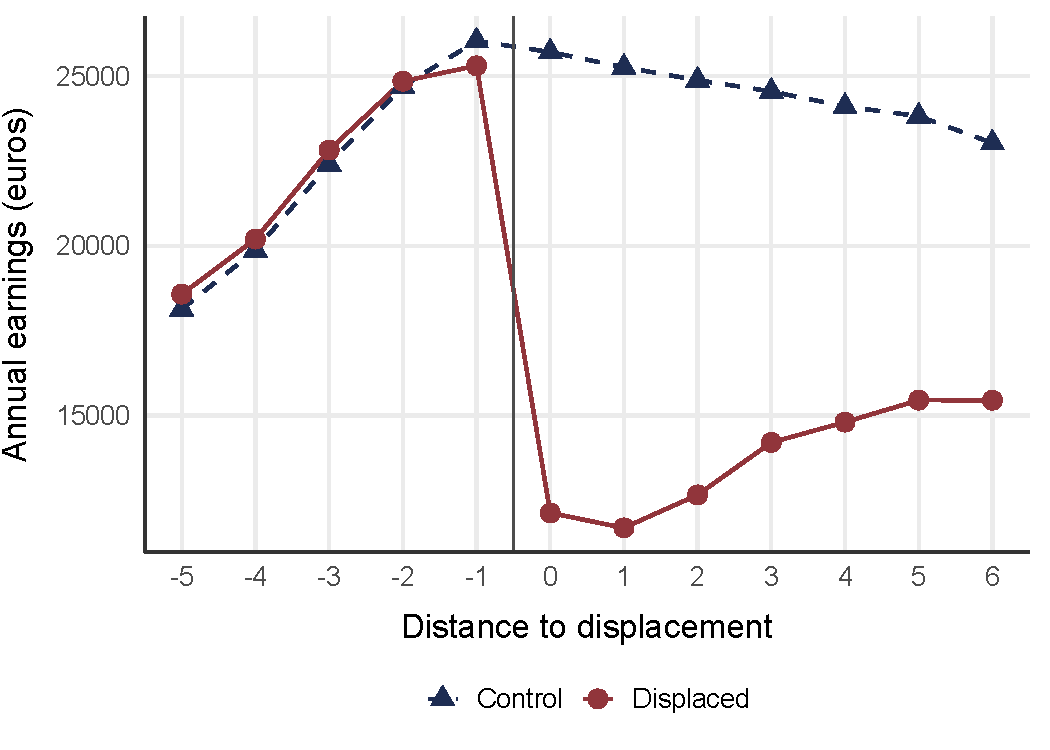
\includegraphics[scale=0.75,max width=\linewidth]{figures/02_descriptive_figures/figure_A15_raw_earnings.pdf}
\floatfoot{\footnotesize{\textsc{Notes}: This figure displays the average annual gross wage in both displaced-workers and control groups. It shows the evolution of gross wage in our sample from $t^D-3$ to $t^D+6$. \textbf{Sample}: The sample contains 20,897 economic dismissals (LE) and as many controls. \textcolor{orange}{[21,132]} \textbf{Outcomes:} Table \ref{apptab:definitions} summarizes variables' definition. \textbf{Specification}: The points displayed are computed as the simple average in annual gross wage by distance to displacement. Non working individuals have wage 0 (as long as they are under 65 and $t<2013$).
}}
\end{figure}


\begin{figure}[h!] 
	\caption{Raw Means on Hours Workers in Control and Treatment Groups\label{fig:raw_mean_hours}} 
	\centering
	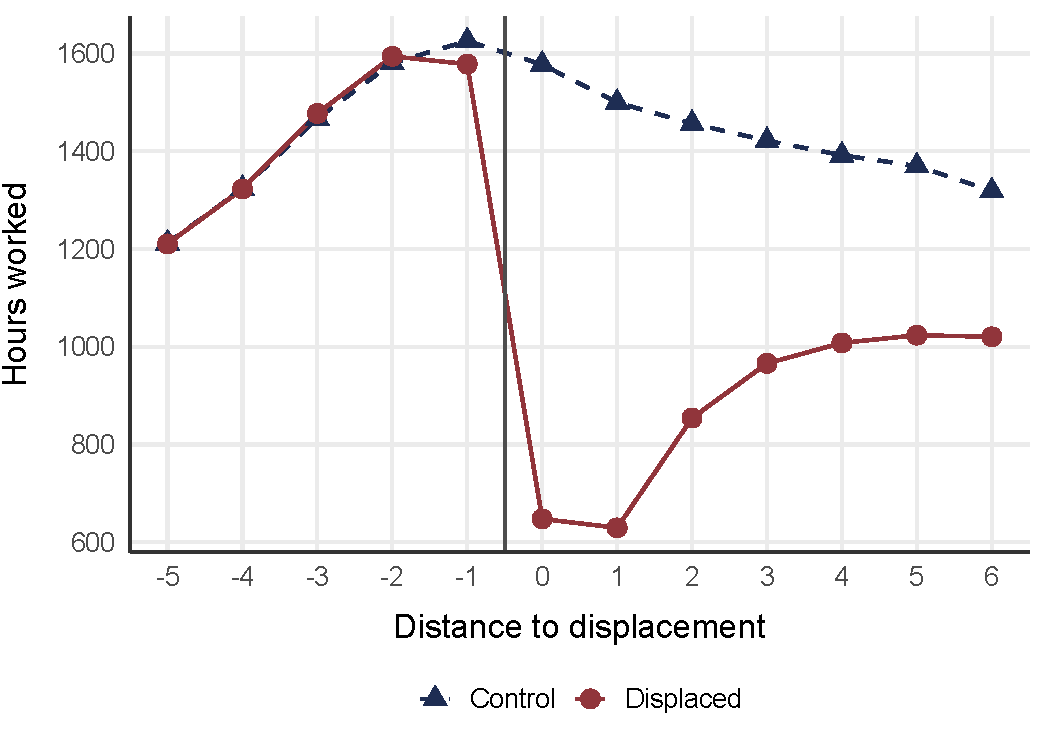
\includegraphics[scale=0.75,max width=\linewidth]{figures/02_descriptive_figures/figure_A16_raw_hours.pdf}
\floatfoot{\footnotesize{\textsc{Notes}: This figure displays the average number of hours worked in both displaced-workers and control groups. It shows the evolution of hours in our sample from $t^D-3$ to $t^D+6$. \textbf{Sample}: The sample contains 20,897 economic dismissals (LE) and as many controls. \textcolor{orange}{[21,132]} \textbf{Outcomes:} Table \ref{apptab:definitions} summarizes variables' definition. \textbf{Specification}: The points displayed are computed as the simple average in annual hours worked by distance to displacement. Non working individuals have hours 0 (as long as they are under 65 and $t<2013$).
}}
\end{figure}




\FloatBarrier
\clearpage

\subsection{Tables}
\FloatBarrier

\begin{table}[h!]
\centering
\caption{Raw firm-level means by type of firm (LE sample, descriptive complement to Table~\ref{tab:firing_hiring_rest})\label{apptab:firing_hiring_means}}
{\footnotesize
\begin{adjustbox}{max width=\linewidth}
\begin{tabular}{lcccccc}\toprule
% Generated from current results_analysis CSV files by master.R, section I (scripts/I-PLOTS_AND_TABLES).
% Table A1; status: ready
% Cell means weighted by n_siren; overlapping firms appear in both rows. Outcome-specific nonmissing denominators are not exported.
% -- means a requested statistic is unavailable; an empty cell means not applicable.
 & (1) & (2) & (3) & (4) & (5) & (6) \\
 & Wage premium & ln(VA/L) & Productivity & ln(labor share) & ln(L) & N (firms) \\
\midrule
Origin firms & 2.429 & 3.704 & -0.037 & -0.127 & 2.688 & 14,115 \\
Destination firms & 2.433 & 4.011 & 0.172 & -0.223 & 3.237 & 5,076 \\
Other firms & 2.340 & 3.743 & -0.070 & -0.318 & 0.976 & 1,897,770 \\

\bottomrule
\end{tabular}
\end{adjustbox}}
\floatfoot{\footnotesize{\textsc{Notes}: Raw firm-level means for three exhaustive groups of firms in the FICUS-FARE panel: (i) origin firms (where displaced workers were employed in $t^D-1$), (ii) destination firms (where displaced workers were employed in $t^D+4$ or $t^D+5$), and (iii) the population of firms that are neither an origin nor a destination of any LE-displaced worker. The Origin and Destination groups overlap in $497$ firms (about $3.5\%$ of origins and $9.7\%$ of destinations) \textcolor{orange}{[R2: 490 firms, since $14{,}115+5{,}076+1{,}897{,}770-1{,}916{,}471=490$ (group sizes in this table, observations in Table~\ref{tab:firing_hiring_rest}); the same identity gives the 497 of R1; the two shares still round to 3.5\% and 9.7\%]}; these firms are counted in both rows. All firm-level outcomes are computed as the within-firm average over $2002$--$2015$. ``Wage premium'' is $\widehat{\psi}_{f}$ from Section~\ref{sec:data:firm:premium}, estimated on the entire panel; productivity is the residual from an OLS regression of value-added on tangible capital and labor with year fixed effects. \textcolor{orange}{The raw means already show that destination firms are more productive than origin firms ($+0.172$ against $-0.037$), and that both groups pay higher wage premia than other firms ($2.433$ and $2.429$ against $2.340$); the premium gap between origin and destination firms highlighted in Table~\ref{tab:firing_hiring_rest} appears once sectors are controlled for.}}}
\end{table}

\FloatBarrier

\begin{table}[h!]
\centering
\caption{Comparison of origin and destination firms, weighted by firm employment (worker-level analogue of Table~\ref{tab:firing_hiring_rest})\label{apptab:firing_hiring_weighted}}
{\footnotesize
\begin{adjustbox}{max width=\linewidth}
\begin{tabular}{llll}\toprule
% Generated from current results_analysis CSV files by master.R, section I (scripts/I-PLOTS_AND_TABLES).
% Table A2; status: ready
% Adjusted R2 and the origin-destination equality-test p-value use the updated exports.
% -- means a requested statistic is unavailable; an empty cell means not applicable.
 & (1) & (2) & (3) \\
 & Wage premium & VA/worker & Productivity \\
\midrule
Destination firm & 0.01958\sym{***} & 0.07059\sym{***} & 0.05514\sym{**} \\
 & (4.11) & (3.39) & (3.00) \\
\addlinespace
Origin firm & 0.04297\sym{***} & 0.01066 & 0.01285 \\
 & (5.39) & (0.97) & (1.46) \\
\addlinespace
\midrule
Observations & 1,916,471 & 1,916,471 & 1,916,471 \\
$R^2$ & 0.173 & 0.338 & 0.269 \\
Adjusted $R^2$ & 0.173 & 0.338 & 0.269 \\
Sector FE & $\surd$ & $\surd$ & $\surd$ \\
P-value Origin-Destination & 0.053 & 0.041 & 0.089 \\

\bottomrule
\end{tabular}
\end{adjustbox}}
\floatfoot{\footnotesize{\textsc{Notes}: This table reproduces the structure of Table~\ref{tab:firing_hiring_rest} columns (1) to (3) for the same outcomes (firm wage premium, value-added per worker, productivity), but the regressions are weighted by firm employment ($\exp(\overline{\ln L_{f}})$ averaged over 2001--2015). Because in a firm-level cross-section the weighted firm-mean coincides with the unweighted worker-level mean, the table is equivalent to running the comparison at the worker level relative to an average worker, as suggested by a referee. The qualitative pattern is preserved relative to Table~\ref{tab:firing_hiring_rest}: origin firms have higher wage premia and lower value added per worker than destination firms. \textcolor{orange}{[``similar magnitudes'' clause dropped on 2026-11-20: the premium gap between origin and destination firms is larger when firms are weighted, as Section~\ref{sec:rolefirm:hiring_firing} now states]} $z$-statistics based on robust standard errors in parentheses. {*} $p<0.05$, {**} $p<0.01$, {***} $p<0.001$.}}
\end{table}

\FloatBarrier

% Added in the R2 revision (Referee 3, point 4): dispersion of firm-level characteristics across firms.
% The tabular is shared with Table R2 of the letter to Referee 3 (Letters/referee3_response.tex).
\begin{table}[h!]\caption{Dispersion of firm-level characteristics across firms, 2002--2015 averages}\label{apptab:dispersion}
	{\footnotesize
	\begin{center}
		\begin{adjustbox}{max width=\linewidth}
		% Generated from current results_analysis CSV files by master.R, section I (scripts/I-PLOTS_AND_TABLES).
% Table A3; status: ready
% Employment-weighted moments; baseline LE effects at +5; percentile approximated from adjacent quartiles.
% -- means a requested statistic is unavailable; an empty cell means not applicable.
\begin{tabular}{lcccc}
\toprule
 & (1) & (2) & (3) & (4) \\
 & Productivity & VA per worker & Labor share & Wage premium \\
\midrule
\multicolumn{5}{l}{\textit{Panel A. Distribution across firms, weighted by employment}} \\
Standard deviation & 0.601 & 0.688 & 0.481 & 0.173 \\
25th percentile & -0.171 & -0.199 & -0.015 & 0.029 \\
Median & 0.090 & 0.097 & 0.194 & 0.119 \\
75th percentile & 0.436 & 0.452 & 0.336 & 0.198 \\
Interquartile range & 0.607 & 0.652 & 0.352 & 0.168 \\
\addlinespace
\multicolumn{5}{l}{\textit{Panel B. Displacement effect at $t^D+5$ (Table~\ref{tab:evstudytable_body}) relative to panel A}} \\
Coefficient at $t^D+5$ & 0.134 & 0.066 & -0.074 & -0.037 \\
Share of the interquartile range & 0.22 & 0.10 & 0.21 & 0.22 \\
In standard-deviation units & 0.22 & 0.10 & 0.15 & 0.22 \\
Percentile reached by a median firm & 60 & 55 & 41 & 40 \\
\midrule
Firms with a non-missing value & 2,346,321 & 2,525,260 & 2,534,596 & 2,054,893 \\
\bottomrule
\end{tabular}

		\end{adjustbox}
	\end{center}}
	\floatfoot{{\footnotesize \textsc{Notes}: Each column reports the distribution across firms of one firm-level characteristic, computed as a within-firm average over 2002--2015. \textcolor{orange}{Each column uses all firms of the FICUS-FARE data with non-missing employment and a non-missing value of that characteristic (last row). Table~\ref{tab:firing_hiring_rest} instead keeps only firms with non-missing values for all its outcomes, hence its smaller sample.} \textit{Productivity} is the residual of an OLS regression of log value added on log tangible capital and log employment with year fixed effects, net of 2-digit sector fixed effects -> \textcolor{red}{without additional 2-digit sector residualization}; \textit{VA per worker} is log value added per worker; \textit{labor share} is the log of total labor costs over value added; \textit{wage premium} is the AKM firm fixed effect estimated over 2002--2015 (Section \ref{sec:data:firm:premium}). All variables are expressed as deviations from their unweighted mean across firms. In panel A firms are weighted by employment. Panel B reports the $t^D+5$ coefficients of Table \ref{tab:evstudytable_body} (panel b for columns 1--3, column (6) of panel a for the wage premium), their absolute value as a share of the employment-weighted interquartile range and in employment-weighted standard-deviation units, and the percentile that a firm initially at the median of panel A would reach after a change equal to the coefficient, obtained by linear interpolation between the median and the adjacent quartile. The event-study outcomes are three-year averages centered on $t^D-4$, which are more dispersed across firms than the fourteen-year averages used here.}}
\end{table}

\FloatBarrier

\begin{table}[h!]
\centering
\caption{Event-study coefficients for firm age and worker mean tenure (LE sample) \label{apptab:firm_age_tenure}}
% Generated from current results_analysis CSV files by master.R, section I (scripts/I-PLOTS_AND_TABLES).
% Table A4; status: ready
% Tenure is mean_tenure_eqtp_ma3_dlag4 under the confirmed baseline rule.
% -- means a requested statistic is unavailable; an empty cell means not applicable.
\begin{tabular}{lcccc}
\toprule
 & $d=-2$ & $d=0$ & $d=2$ & $d=5$ \\
\midrule
Firm age (years) & +0.000 & -0.609*** & -2.124*** & -1.931*** \\
 &  & (0.076) & (0.218) & (0.337) \\
Mean worker tenure (years) & +0.000 & -0.110*** & -0.685*** & -0.444*** \\
 &  & (0.009) & (0.033) & (0.044) \\
\bottomrule
\end{tabular}

\floatfoot{\footnotesize{\textsc{Notes}: Event-study coefficients of the displacement indicator on two firm-level outcomes for the LE sample: the destination firm's age in years (defined as the year minus year of creation) and the firm-level mean of worker tenure in years. $d=-2$ is the reference period (coefficient implicitly zero). Standard errors clustered at the worker level in parentheses; significance: $^{*}p<0.10$, $^{**}p<0.05$, $^{***}p<0.01$. The destination--origin gap of $\approx -1.5$ years on firm age and $\approx +0.55$ years on mean tenure at $t^D+5$ is too small to substitute for the bargaining-power channel discussed in the paper.}}
\end{table}

\FloatBarrier

% The descriptive statistics table (former Table A4, label tab:desc:AllLE) was moved to the main text in the R2 revision (Referee 3, point 1).

\begin{table}
	\caption{Definition of datasets}\label{apptab:datasets}
	{\scriptsize% Generated from the current results_analysis CSV files by plots_tables/run_all.R.
% Table A5; status: ready
% Text definitions retained; no numerical regression results copied.
% -- means a requested statistic is unavailable; an empty cell means not applicable.
{
\begin{tabularx}{\textwidth}{ZXlZ}
\hline
Dataset & Description & Period & Main use \\
\hline
&&&\\
DADS postes & (\textit{Déclaration Annuelle des Données Sociales}) is a matched employer-employee dataset coming from the administrative declaration that all employers report annually to social security authorities and tax administration; we restrict the sample to companies governed by private law. DADS contains information on firms and establishments (unique identifier; size; industry) as well as on each employees’ job (occupation, wage, hours worked, start and end date, type of contract, etc.). Firm (SIREN) unique id. & ]2001-2015[ & Compute firm premium \\
\rowcolor{lightgray} Panel DADS & Is a panel version of DADS (cf. above) containing a random sample of 1/12 of the universe of workers. Firm (SIREN) and worker unique id. & ]2001-2015[ & Workers' trajectories. Samples construction. \\
FH-DADS  & Matches the Panel DADS (cf. above) to the FH (Fichier Historique) data, an historical administrative file produced by the national unemployment agency (\textit{Pôle Emploi}) which records individuals’ unemployment spells. Any job seeker claiming unemployment benefits appears in the FH, which contains information about date of registration, duration and level of unemployment benefits. Firm (SIREN) and worker unique id. & [2002-2012] & Identify workers laid-off for economic reasons \\
\rowcolor{lightgray} FICUS-FARE  & Is a nearly exhaustive administrative dataset built from the corporate tax returns and the social security declaration of the universe of firms in the non-financial corporate sector. We use the FICUS-FARE panel as processed by \citet{burstein_etal_2025}. Firm (SIREN) unique id. & ]2001-2015[ & Firms' productivity, value-added, etc. \\
D@ccord  & D@ccord data reports information about firms' negotiations regarding collective agreement. In France, firms are required by the labor law to report any negotiation (successfull or not). The Ministry of Labor then builds this data set. Useful information contains: the matter of negotiation (wages, hours, etc.), the parties negotiating or signing (trade union, etc.), outcome, date of signature. Firm (SIREN) unique id. & [2005-2007[ & Collective agreements. \\
\rowcolor{lightgray} Workplace election  & Data reports the results of all workplace election held in France over 2009-2012. The election is characterized by its electoral college and its outcome (share of voters, vote by trade union, etc.) Firm (SIREN) unique id. & [2009-2012] & Workplace election turnout and failure. \\
&&&\\ \hline
\end{tabularx}
}







}
	\floatfoot{{\footnotesize \textsc{Notes}: This table provides a summary of the main datasets.}}
\end{table}



\begin{table}
	\caption{Definition of main variables (1/2)}\label{apptab:definitions}
	{\footnotesize% Generated from the current results_analysis CSV files by plots_tables/run_all.R.
% Table A6; status: ready
% Text definitions retained; no numerical regression results copied.
% -- means a requested statistic is unavailable; an empty cell means not applicable.
{
%\def\sym#1{\ifmmode^{#1}\else\(^{#1}\)\fi}
\begin{tabularx}{\textwidth}{ZXlZ}
	%\begin{tabular}{l*{3}{c}}
\hline
%\multicolumn{1}{c}{Outcome}&\multicolumn{1}{c}{Definition}&\multicolumn{1}{c}{Period}&\multicolumn{1}{c}{Source}\\
Outcome & Definition & Period & Source\\
\hline
&&&\\
\multicolumn{4}{l}{\textbf{Worker}} \\ 
Employed  & Indicator taking value 1 if the workers has worked (positive hours and earning). & $t$ & DADS panel \\
\rowcolor{lightgray} Earnings & Total of gross wages earned by the worker. Missing data is coded 0. & $t$ & DADS panel \\
Hours worked  & Total hours worked by the worker. Missing data is coded 0.  & $t$ & DADS panel \\
\rowcolor{lightgray} Hourly wage (or wage rate)  & Earnings over Hours. & $t$ & DADS panel \\
(log) Earnings  & Log of: Earnings (cf. above) & $t$& DADS panel\\
\rowcolor{lightgray} (log) Hours  & Log of: Hours (cf. above)  & $t$& DADS panel \\
(log) Hourly wage & Log of: Hourly wage (cf. above) & $t$ & DADS panel \\
\rowcolor{lightgray} \# employees  & Number of workers in the firm on December 31st. & $t$ & DADS panel \\
Premium $\widehat{\psi}_{J(i, t)}$ & Firm fixed effect associated with the firm in an AKM framework presented in equation \ref{eq:akm_basics}. & 2002-2015$^{a}$ & DADS  \\
&&&\\
\multicolumn{4}{l}{\textbf{Firm}} \\
\rowcolor{lightgray} Productivity & Residual of an OLS regression of \textcolor{red}{log} value-added on the \textcolor{red}{log of} book value of tangible capital and \textcolor{orange}{the log of employment} with year fixed effect\textcolor{orange}{s}. & $t^D-4^{a,b}$ & FICUS-FARE \\
VA / Worker & Computed as value-added over reported employment. & $t^D - 4^{a, b}$ & FICUS-FARE \\ 
\rowcolor{lightgray} Labor share & Total labor cost over value-added. & $t^D - 4^{a, b}$ & FICUS-FARE \\
Manufacturing & Indicator for firms whose sector is (at least once over the period) manufacturing. &2002-2015$^{a}$ & FICUS-FARE \\&&&\\
\hline
\end{tabularx}
}
%$[t^D-7;t^D-3]$

}
\end{table}
\begin{table}
	\caption*{Definition of main variables (2/2)}
	{\footnotesize% Generated from the current results_analysis CSV files by plots_tables/run_all.R.
% Table A6; status: ready
% Text definitions retained; no numerical regression results copied.
% -- means a requested statistic is unavailable; an empty cell means not applicable.
{
	%\def\sym#1{\ifmmode^{#1}\else\(^{#1}\)\fi}
\begin{tabularx}{\textwidth}{ZXlZ}
		%\begin{tabular}{l*{3}{c}}
		\hline
		%\multicolumn{1}{c}{Outcome}&\multicolumn{1}{c}{Definition}&\multicolumn{1}{c}{Period}&\multicolumn{1}{c}{Source}\\
		Outcome & Definition & Period & Source\\
		\hline
		&&&\\
		\multicolumn{4}{l}{\textbf{Collective agreements (more in \ref{appsec:accord_data})}} \\
\rowcolor{lightgray} 		Wage agreement indicator & Indicator taking value 1 if the firm has signed (at least) one agreement relative to wages, and 0 otherwise. & 2005-2007$^{a}$ & D@ccord \\
		\# Wage agreement & Number of wages agreement signed by the firm. & 2005-2007$^{a}$ & D@ccord \\
\rowcolor{lightgray} 		Wage failure indicator & Indicator taking value 1 if the firm has failed to conclude (at least) one negotiation relative to wages, and 0 otherwise. & 2005-2007$^{a}$ & D@ccord \\
		Hours agreement indicator & Indicator taking value 1 if the firm has signed (at least) one agreement relative to hours and working time, and 0 otherwise. & 2005-2007$^{a}$ & D@ccord \\
		&&&\\
		\multicolumn{4}{l}{\textbf{Elections (more in \ref{appsec:elec_data})}} \\
		Average turnout         & Worker-weighted average participation of electors in firm-specific professional elections. & 2009-2012$^{a}$ & Ministère du Travail \\
\rowcolor{lightgray} 		Failed (share workers)   & Share of firm's workers who were electors of a failed election (i.e. no trade union ran). & 2009-2012$^{a}$ & Ministère du Travail \\
		CGT (share workers) & Share of firm's workers who were electors in an election were a CGT representative received more than 10\%. & 2009-2012$^{a}$ & Ministère du Travail \\	
		&&&\\
		\hline
	\end{tabularx}
}


}
	\floatfoot{{\footnotesize \textsc{Notes}: This table provides a summary of the main variables and their definition. Throughout the paper, variables' name can sometimes be abbreviated.} \\
	${^a}$Outcome for firm $J$ is computed over the given period; in $t$, worker $i$ is then assigned $J(i,t)$, the value of the firm he works in $t$. \\
	${^b}$For Tables \ref{tab:firm_fe_desc} and \ref{tab:firm_fe_nego}, firm outcomes are computed as averages over 2002-2015.
    }
\end{table}

\begin{table}\caption{Event-study estimates in the sample of workers dismissed for economic reasons: Worker-level outcomes\label{apptab:evstudy_worker_outcomes}}	{\footnotesize
		\begin{adjustbox}{max width=\linewidth}
\begin{tabular}{l|lllllll}\toprule
			% Generated from current results_analysis CSV files by master.R, section I (scripts/I-PLOTS_AND_TABLES).
% Table A7; status: ready
% 
% -- means a requested statistic is unavailable; an empty cell means not applicable.
& \multicolumn{2}{l}{Outcome in levels} & \multicolumn{5}{l}{Outcomes in log} \\ \cmidrule[1.5pt](lr){2-3} \cmidrule[1.5pt](lr){4-8}
 & (1) & (2) & (3) & (4) & (5) & (6) & (7) \\
Time to displ. & Employed & Earnings & Earnings & Hours & Hourly wage & Premium & Ratio (6)/(5) \\
\midrule
$d=-3$ & 0.000 & 271 & -0.024 & -0.033 & 0.012 & 0.000 & 0.004 \\
 & (0.000) & (154) & (0.007) & (0.007) & (0.002) & (0.001) &  \\
$d=-2$ & REF & REF & REF & REF & REF & REF &  \\
 &  &  &  &  &  &  &  \\
$d=-1$ & 0.000 & -875 & -0.058 & -0.066 & 0.005 & 0.000 & 0.001 \\
 & (0.000) & (126) & (0.005) & (0.005) & (0.002) & (0.000) &  \\
$d=0$ & -0.164 & -13,731 & -0.932 & -0.953 & 0.047 & -0.001 & -0.027 \\
 & (0.003) & (264) & (0.009) & (0.009) & (0.004) & (0.001) &  \\
$d=1$ & -0.315 & -13,687 & -0.791 & -0.773 & -0.096 & -0.022 & 0.232 \\
 & (0.004) & (294) & (0.011) & (0.012) & (0.004) & (0.002) &  \\
$d=2$ & -0.219 & -12,267 & -0.541 & -0.454 & -0.106 & -0.029 & 0.274 \\
 & (0.004) & (326) & (0.012) & (0.012) & (0.004) & (0.002) &  \\
$d=3$ & -0.167 & -10,496 & -0.433 & -0.331 & -0.108 & -0.030 & 0.279 \\
 & (0.004) & (358) & (0.012) & (0.012) & (0.004) & (0.002) &  \\
$d=4$ & -0.146 & -9,453 & -0.360 & -0.257 & -0.108 & -0.033 & 0.305 \\
 & (0.005) & (385) & (0.014) & (0.014) & (0.005) & (0.003) &  \\
$d=5$ & -0.139 & -8,690 & -0.318 & -0.231 & -0.101 & -0.037 & 0.372 \\
 & (0.006) & (340) & (0.017) & (0.017) & (0.006) & (0.003) &  \\
$d=6$ & -0.118 & -7,961 & -0.322 & -0.228 & -0.106 & -0.035 & 0.328 \\
 & (0.009) & (405) & (0.022) & (0.021) & (0.007) & (0.004) &  \\
\midrule
$N$ & 385,642 & 385,578 & 351,292 & 346,450 & 342,843 & 335,861 &  \\
\# treated & 21,132 & 21,132 & 21,132 & 21,132 & 21,132 & 21,132 &  \\
$R^2$ & 0.350 & 0.601 & 0.532 & 0.395 & 0.718 & 0.801 &  \\
\bottomrule		
	\end{tabular}
\end{adjustbox}}
	
	
	\floatfoot{{\footnotesize  \textsc{Notes}: This table presents event-study estimates of the cost of job displacement for a sample of workers dismissed for economic reasons (LE) ---see equation (\ref{eq:main_estimating_equation}) and associated text for more details on the specification. 
	\textbf{Outcomes}: Table \ref{apptab:definitions} summarizes variables' definition. 
 	\textbf{Worker-level}: employed is an indicator taking value 1 if individual has positive hours and earnings at time $t$. Earnings are gross earnings in year $t$. Hourly wage is the ratio of earnings over hours worked. Column (3) to (5) are built on logarithmic transformation of those outcomes. Wage premia are estimated, following the AKM framework, as firm-fixed effects in a two-way regression of log-hourly wage on firm and worker fixed effects---see section \ref{sec:data:firm:premium} for more details. Ratio is the ratio of (the coefficients of) premium over hourly wage. \textbf{Standard errors}: robust standard errors clustered at the worker-level.
}}
\end{table}

\begin{table}\caption{Event-study estimates in the sample of workers dismissed for economic reasons: Firm-level outcomes\label{apptab:evstudy_firm_outcomes}}	{\footnotesize
		\begin{adjustbox}{max width=\linewidth}
\begin{tabular}{l|lllll}\toprule
			% Generated from current results_analysis CSV files by master.R, section I (scripts/I-PLOTS_AND_TABLES).
% Table A8; status: ready
% LE agreement estimates intentionally stop at +4; later agreement cells are blank, as in the paper.
% -- means a requested statistic is unavailable; an empty cell means not applicable.
& \multicolumn{3}{l}{Firm outcomes} & \multicolumn{2}{l}{Negotiation variables} \\
\cmidrule[1.5pt](lr){2-4}\cmidrule[1.5pt](lr){5-6}
 & (1) & (2) & (3) & (4) & (5) \\
Time to displ. & Productivity & VA / Worker & Labor share & Wage Agr. ind. & Election turnout \\
\midrule
$d=-3$ & 0.001 & -0.008 & 0.004 & 0.017 & -0.007 \\
 & (0.002) & (0.002) & (0.001) & (0.003) & (0.001) \\
$d=-2$ & REF & REF & REF & REF & REF \\
 &  &  &  &  &  \\
$d=-1$ & -0.000 & -0.000 & 0.000 & -0.000 & 0.000 \\
 & (0.000) & (0.000) & (0.000) & (0.000) & (0.000) \\
$d=0$ & 0.035 & 0.020 & -0.013 & -0.018 & -0.018 \\
 & (0.003) & (0.002) & (0.002) & (0.004) & (0.002) \\
$d=1$ & 0.159 & 0.019 & -0.038 & -0.076 & -0.165 \\
 & (0.008) & (0.008) & (0.006) & (0.013) & (0.010) \\
$d=2$ & 0.129 & 0.022 & -0.047 & -0.076 & -0.136 \\
 & (0.008) & (0.009) & (0.007) & (0.014) & (0.010) \\
$d=3$ & 0.131 & 0.050 & -0.064 & -0.080 & -0.112 \\
 & (0.009) & (0.009) & (0.007) & (0.016) & (0.010) \\
$d=4$ & 0.143 & 0.071 & -0.072 & -0.065 & -0.095 \\
 & (0.010) & (0.011) & (0.008) & (0.022) & (0.011) \\
$d=5$ & 0.134 & 0.066 & -0.074 &  & -0.086 \\
 & (0.012) & (0.012) & (0.010) &  & (0.012) \\
$d=6$ & 0.128 & 0.066 & -0.064 &  & -0.084 \\
 & (0.015) & (0.017) & (0.013) &  & (0.013) \\
\midrule
$N$ & 246,416 & 254,418 & 257,706 & 90,120 & 90,252 \\
\# treated & 21,132 & 21,132 & 21,132 & 16,512 & 17,071 \\
$R^2$ & 0.863 & 0.863 & 0.817 & 0.832 & 0.899 \\
\bottomrule		
	\end{tabular}
\end{adjustbox}}


	\floatfoot{{\footnotesize  \textsc{Notes}: This table presents event-study estimates of the cost of job displacement for a sample of workers dismissed for economic reasons (LE) ---see equation (\ref{eq:main_estimating_equation}) and associated text for more details on the specification. \textbf{Comment on timing}: Firm-level outcomes are computed as three-year averages centered on $t^D-4$ (i.e.\ over $t^D-5$, $t^D-4$, and $t^D-3$), while displacements occur from 2005 to 2012. Accordingly, event-study coefficients reflect the movement of displaced workers to firms with different initial characteristics and \textit{not} changes within-firm in such characteristics. \textbf{Outcomes}: Table \ref{apptab:definitions} summarizes variables' definition.
	\textbf{Firm-level}: Value added per worker is computed as value added over reported employment. Productivity is obtained as the residual of an OLS regression of value-added on the book value of tangible capital and labor with year fixed effects. The labor share is computed as total labor cost over value-added. \textbf{Definition of firm-level outcomes related to labor relations}: In column (4) the dependent variable Wage agreement indicator refers to collective wage agreement and is an indicator equal to 1 when firms signed at least one agreement related to wages over the period 2005 to 2007. The variable in column (5) Election turnout captures each firm's average turnout at 2009--2012 workplace elections. More details are provided in Section \ref{sec:Nego}.
	\textbf{Standard errors}: robust standard errors clustered at the worker-level.

}}
\end{table}


\begin{table}[h!]\caption{Event-study estimates using the \emph{unrestricted} AKM firm wage premium, without excluding any LE or MLO30 displaced worker (LE sample)} %(\texttt{fe0215\_god2}) %  worker-level outcomes
\label{tab:paper_R_evstudy_god2} 
{\footnotesize
\begin{adjustbox}{max width=\linewidth}
\begin{tabular}{l|lllllll}\toprule
% Generated from current results_analysis CSV files by master.R, section I (scripts/I-PLOTS_AND_TABLES).
% Table A9; status: ready
% 
% -- means a requested statistic is unavailable; an empty cell means not applicable.
& \multicolumn{2}{l}{Outcome in levels} & \multicolumn{5}{l}{Outcomes in log} \\ \cmidrule[1.5pt](lr){2-3} \cmidrule[1.5pt](lr){4-8}
 & (1) & (2) & (3) & (4) & (5) & (6) & (7) \\
Time to displ. & Employed & Earnings & Earnings & Hours & Hourly wage & Premium & Ratio (6)/(5) \\
\midrule
$d=-3$ & 0.000 & 271 & -0.024 & -0.033 & 0.012 & -0.000 & -0.011 \\
 & (0.000) & (154) & (0.007) & (0.007) & (0.002) & (0.001) &  \\
$d=-2$ & REF & REF & REF & REF & REF & REF &  \\
 &  &  &  &  &  &  &  \\
$d=-1$ & 0.000 & -875 & -0.058 & -0.066 & 0.005 & 0.000 & 0.002 \\
 & (0.000) & (126) & (0.005) & (0.005) & (0.002) & (0.000) &  \\
$d=0$ & -0.164 & -13,731 & -0.932 & -0.953 & 0.047 & -0.003 & -0.056 \\
 & (0.003) & (264) & (0.009) & (0.009) & (0.004) & (0.001) &  \\
$d=1$ & -0.315 & -13,687 & -0.791 & -0.773 & -0.096 & -0.045 & 0.464 \\
 & (0.004) & (294) & (0.011) & (0.012) & (0.004) & (0.002) &  \\
$d=2$ & -0.219 & -12,267 & -0.541 & -0.454 & -0.106 & -0.050 & 0.474 \\
 & (0.004) & (326) & (0.012) & (0.012) & (0.004) & (0.002) &  \\
$d=3$ & -0.167 & -10,496 & -0.433 & -0.331 & -0.108 & -0.052 & 0.477 \\
 & (0.004) & (358) & (0.012) & (0.012) & (0.004) & (0.002) &  \\
$d=4$ & -0.146 & -9,453 & -0.360 & -0.257 & -0.108 & -0.054 & 0.501 \\
 & (0.005) & (385) & (0.014) & (0.014) & (0.005) & (0.002) &  \\
$d=5$ & -0.139 & -8,690 & -0.318 & -0.231 & -0.101 & -0.059 & 0.587 \\
 & (0.006) & (340) & (0.017) & (0.017) & (0.006) & (0.003) &  \\
$d=6$ & -0.118 & -7,961 & -0.322 & -0.228 & -0.106 & -0.059 & 0.554 \\
 & (0.009) & (405) & (0.022) & (0.021) & (0.007) & (0.004) &  \\
\midrule
$N$ & 385,642 & 385,578 & 351,292 & 346,450 & 342,843 & 338,026 &  \\
\# treated & 21,132 & 21,132 & 21,132 & 21,132 & 21,132 & 21,132 &  \\
$R^2$ & 0.350 & 0.601 & 0.532 & 0.395 & 0.718 & 0.809 &  \\

\bottomrule
\end{tabular}
\end{adjustbox}}
\par\medskip
\floatfoot{\footnotesize\textsc{Notes}: Sensitivity exhibit accompanying Figure~\ref{fig:paper_R_wage_decomposition_god2}, reporting the LE event-study under the unrestricted AKM (no exclusion of LE/MLO trajectories). Column~(6) is the firm wage premium estimated on the full firm-year panel without any contamination correction; column~(7) is the implied firm-premium share of the hourly-wage scar, $\beta_{\mathrm{AKM}}/\beta_{\mathrm{hourly}}$, at each horizon. Comparing column~(7) here to column~(7) of the contamination-corrected Table~\ref{apptab:evstudy_worker_outcomes} (LE) shows the magnitude of the AKM contamination correction: at $t^D+2$ the share falls from $51\%$ (here) to $35\%$ (corrected), at $t^D+5$ from $61\%$ to $43\%$, and at $t^D+6$ from $59\%$ to $39\%$ \textcolor{orange}{[R2: 47\% to 27\% at $t^D+2$, 59\% to 37\% at $t^D+5$ and 55\% to 32\% at $t^D+6$ (this table, col. 7: 0.470, 0.586, 0.545; Appendix Table~\ref{apptab:evstudy_worker_outcomes}, col. 7: 0.272, 0.371, 0.322)]}. Robust standard errors clustered at the worker level in parentheses.}
\end{table}




\begin{table}[h!]\caption{Firm-level correlates of firm wage premium}\label{tab:firm_fe_desc}
	{\footnotesize
		\begin{adjustbox}{max width=\linewidth}
\begin{tabular}{lllllllll}\toprule
			% Generated from current results_analysis CSV files by master.R, section I (scripts/I-PLOTS_AND_TABLES).
% Table A10; status: ready
% Unrestricted AKM; unweighted; minmax_year-clustered errors.
% -- means a requested statistic is unavailable; an empty cell means not applicable.
 & (1) & (2) & (3) & (4) & (5) & (6) & (7) & (8) \\
\midrule
Employees & 0.040 &  & 0.038 & 0.037 &  &  & 0.037 & 0.032 \\
 & (0.001) &  & (0.002) & (0.002) &  &  & (0.002) & (0.001) \\
\addlinespace
VA &  & 0.080 &  &  &  &  &  &  \\
 &  & (0.008) &  &  &  &  &  &  \\
\addlinespace
VA per worker &  &  & 0.087 &  &  &  &  &  \\
 &  &  & (0.011) &  &  &  &  &  \\
\addlinespace
Productivity &  &  &  & 0.086 &  &  & 0.087 & 0.070 \\
 &  &  &  & (0.013) &  &  & (0.013) & (0.010) \\
\addlinespace
Age $>10$ years &  &  &  &  & 0.023 &  & 0.001 & 0.003 \\
 &  &  &  &  & (0.003) &  & (0.002) & (0.002) \\
\addlinespace
Manufacturing &  &  &  &  &  & 0.032 & 0.008 &  \\
 &  &  &  &  &  & (0.004) & (0.003) &  \\
\addlinespace
\midrule
Sector FE &  &  &  &  &  &  &  & $\surd$ \\
Observations & 45,151 & 45,151 & 45,151 & 45,151 & 45,151 & 45,151 & 45,151 & 45,151 \\
$R^2$ & 0.148 & 0.218 & 0.223 & 0.219 & 0.014 & 0.017 & 0.220 & 0.294 \\
Adjusted $R^2$ & 0.147 & 0.216 & 0.221 & 0.218 & 0.012 & 0.014 & 0.218 & 0.292 \\
\bottomrule
	\end{tabular}
\end{adjustbox}}
	\floatfoot{{\footnotesize  \textsc{Notes}: This table presents cross-sectional regressions of firm wage premium on firm-level characteristics. The dependent variable is the AKM firm fixed effect estimated over 2002--2015 with no restriction on displaced workers. \textbf{Sample}: the estimation sample comprises all firms that are present in our LE analysis, either as a firm displacing workers or as a firm employing a matched control worker (the equivalent table for the MLO30 sample shows very similar correlations and is available upon request). \textbf{Outcomes}: Table~\ref{apptab:definitions} summarizes variables' definition. Productivity, size (employees), value-added and value-added per worker are expressed in logs and are averaged over the 2002--2015 period. Firm-level correlates are net of fixed effects for the firm's observed entry and exit years in FARE, so as to remove differences in means mechanically induced by differences in the period over which firms are observed. Productivity is obtained as the residual of an OLS regression of value-added on the book value of tangible capital and labor with year fixed effects. Age $>10$~years is a dummy indicating whether the firm was created before~1994 (or, equivalently, whether the firm is more than ten years old at the start of the AKM estimation window). Manufacturing is a dummy taking value~1 if the firm was in the manufacturing industry at least once over the period (computed as the maximum of the \textit{Manufacturing} dummy across years). Column~(8) adds 2-digit sector fixed effects. Standard errors, clustered at the observed entry-exit cohort level, are reported in parentheses.}}
\end{table}
%			  {*} \(p<0.10\), {**} \(p<0.05\), {***} \(p<0.01\)


\begin{table}[h!]\caption{Election and bargaining correlates of firm wage premium}\label{tab:firm_fe_nego}
	{\footnotesize
	\begin{adjustbox}{max width=\linewidth}
\begin{tabular}{lllllll}\toprule
			% Generated from current results_analysis CSV files by master.R, section I (scripts/I-PLOTS_AND_TABLES).
% Table A11; status: ready
% Uses LE-specific default acco_alt/election samples, not a pooled LE+MLO regression. Caption needs corresponding sample wording.
% -- means a requested statistic is unavailable; an empty cell means not applicable.
 & (1) & (2) & (3) & (4) & (5) & (6) \\
\midrule
Wage agreement ind. & 0.119 & 0.011 & 0.086 &  &  &  \\
 & (0.005) & (0.002) & (0.003) &  &  &  \\
\addlinespace
Election turnout &  &  &  & 0.054 & 0.063 & 0.021 \\
 &  &  &  & (0.006) & (0.006) & (0.003) \\
\addlinespace
Employees &  & 0.036 &  &  & 0.011 &  \\
 &  & (0.001) &  &  & (0.001) &  \\
\addlinespace
\midrule
Sector FE &  &  & $\surd$ &  &  & $\surd$ \\
Observations & 34,704 & 34,704 & 34,704 & 6,837 & 6,837 & 6,837 \\
$R^2$ & 0.055 & 0.149 & 0.222 & 0.030 & 0.045 & 0.235 \\
Adjusted $R^2$ & 0.053 & 0.147 & 0.218 & 0.019 & 0.034 & 0.217 \\
\bottomrule
	\end{tabular}
\end{adjustbox}}
	\floatfoot{{\footnotesize  \textsc{Notes}: This table presents a cross-sectional regression of firm wage premium (estimated over 2002--2015, with no restriction on displaced workers) on firm-level negotiation characteristics over the period of observations (2005-2007 for collective agreements, 2009-2012 for professional elections). \textbf{Sample} This estimation sample comprises all firms that are present either in our LE or MLO analysis, either as a firm displacing workers or as a firm employing a matched control worker. \textbf{Outcomes}: Table \ref{apptab:definitions} summarizes variables' definition. Wage agreement indicator is an indicator taking value 1 if the firm has signed at least one agreement relative to wages over the 2005-2007 period. Election turnout is the average turnout at professional elections in the firm over 2009-2012. Employees is the log of average number of workers in the firm over 2002--2015. Sectors fixed-effects are based on a 2-digit sectoral classification. Robust standard errors in parentheses. }}
\end{table}
	%			  {*} \(p<0.10\), {**} \(p<0.05\), {***} \(p<0.01\)



\begin{table}\caption{Event-study estimates in the mass-layoff sample: Worker-level outcomes\label{apptab:evstudy_worker_outcomes_mlo}}	{\footnotesize
		\begin{adjustbox}{max width=\linewidth}
\begin{tabular}{l|lllllll}\toprule
			% Generated from current results_analysis CSV files by master.R, section I (scripts/I-PLOTS_AND_TABLES).
% Table A12; status: ready
% 
% -- means a requested statistic is unavailable; an empty cell means not applicable.
& \multicolumn{2}{l}{Outcome in levels} & \multicolumn{5}{l}{Outcomes in log} \\ \cmidrule[1.5pt](lr){2-3} \cmidrule[1.5pt](lr){4-8}
 & (1) & (2) & (3) & (4) & (5) & (6) & (7) \\
Time to displ. & Employed & Earnings & Earnings & Hours & Hourly wage & Premium & Ratio (6)/(5) \\
\midrule
$d=-3$ & -0.001 & -90 & 0.002 & -0.002 & 0.004 & 0.000 & 0.095 \\
 & (0.001) & (116) & (0.006) & (0.006) & (0.002) & (0.000) &  \\
$d=-2$ & REF & REF & REF & REF & REF & REF &  \\
 &  &  &  &  &  &  &  \\
$d=-1$ & 0.004 & -1,833 & -0.101 & -0.117 & 0.014 & -0.000 & -0.006 \\
 & (0.001) & (93) & (0.004) & (0.004) & (0.002) & (0.000) &  \\
$d=0$ & -0.179 & -14,599 & -0.580 & -0.640 & 0.052 & -0.009 & -0.178 \\
 & (0.003) & (208) & (0.007) & (0.007) & (0.004) & (0.001) &  \\
$d=1$ & -0.190 & -10,199 & -0.345 & -0.293 & -0.057 & -0.037 & 0.652 \\
 & (0.004) & (231) & (0.007) & (0.007) & (0.003) & (0.001) &  \\
$d=2$ & -0.133 & -7,877 & -0.240 & -0.178 & -0.065 & -0.043 & 0.651 \\
 & (0.004) & (233) & (0.008) & (0.007) & (0.003) & (0.001) &  \\
$d=3$ & -0.099 & -6,896 & -0.196 & -0.131 & -0.069 & -0.044 & 0.632 \\
 & (0.004) & (305) & (0.008) & (0.007) & (0.004) & (0.002) &  \\
$d=4$ & -0.083 & -6,097 & -0.183 & -0.112 & -0.074 & -0.044 & 0.587 \\
 & (0.004) & (272) & (0.008) & (0.007) & (0.004) & (0.002) &  \\
$d=5$ & -0.081 & -5,645 & -0.159 & -0.091 & -0.068 & -0.044 & 0.642 \\
 & (0.004) & (283) & (0.008) & (0.007) & (0.005) & (0.002) &  \\
$d=6$ & -0.071 & -4,713 & -0.157 & -0.090 & -0.068 & -0.043 & 0.640 \\
 & (0.004) & (289) & (0.009) & (0.007) & (0.006) & (0.002) &  \\
\midrule
$N$ & 413,672 & 413,672 & 361,776 & 369,197 & 361,776 & 364,766 &  \\
\# treated & 17,946 & 17,946 & 17,946 & 17,946 & 17,946 & 17,946 &  \\
$R^2$ & 0.355 & 0.629 & 0.607 & 0.378 & 0.747 & 0.708 &  \\
\bottomrule		
	\end{tabular}
\end{adjustbox}}
	
	
	\floatfoot{{\footnotesize  \textsc{Notes}: This table presents event-study estimates of the cost of job displacement for a sample of workers displaced in a mass layoff (MLO) ---see equation (\ref{eq:main_estimating_equation}) and associated text for more details on the specification. 
		\textbf{Outcomes}: Table \ref{apptab:definitions} summarizes variables' definition. 
		\textbf{Worker-level}: employed is an indicator taking value 1 if individual has positive hours and earnings at time $t$. Earnings are gross earnings in year $t$. Hourly wage is the ratio of earnings over hours worked. Column (3) to (5) are built on logarithmic transformation of those outcomes. Wage premia are estimated, following the AKM framework, as firm-fixed effects in a two-way regression of log-hourly wage on firm and worker fixed effects---see section \ref{sec:data:firm:premium} for more details.  Ratio is the ratio of (the coefficients of) premium over hourly wage. \textbf{Standard errors}: robust standard errors clustered at the worker-level.}}
\end{table}

\begin{table}\caption{Event-study estimates in the mass-layoff sample: Firm-level outcomes\label{apptab:evstudy_firm_outcomes_mlo}}	{\footnotesize
		\begin{adjustbox}{max width=\linewidth}
\begin{tabular}{l|lllll}\toprule
			% Generated from current results_analysis CSV files by master.R, section I (scripts/I-PLOTS_AND_TABLES).
% Table A13; status: ready
% MLO bargaining models use their exported support through +6.
% -- means a requested statistic is unavailable; an empty cell means not applicable.
& \multicolumn{3}{l}{Firm outcomes} & \multicolumn{2}{l}{Negotiation variables} \\
\cmidrule[1.5pt](lr){2-4}\cmidrule[1.5pt](lr){5-6}
 & (1) & (2) & (3) & (4) & (5) \\
Time to displ. & Productivity & VA / Worker & Labor share & Wage Agr. ind. & Election turnout \\
\midrule
$d=-3$ & 0.001 & 0.000 & -0.000 & 0.000 & -0.001 \\
 & (0.001) & (0.001) & (0.001) & (0.001) & (0.000) \\
$d=-2$ & REF & REF & REF & REF & REF \\
 &  &  &  &  &  \\
$d=-1$ & 0.002 & 0.001 & -0.001 & -0.001 & 0.000 \\
 & (0.001) & (0.001) & (0.001) & (0.001) & (0.000) \\
$d=0$ & 0.032 & 0.020 & -0.012 & -0.001 & -0.027 \\
 & (0.003) & (0.003) & (0.002) & (0.004) & (0.002) \\
$d=1$ & 0.141 & 0.077 & -0.063 & -0.051 & -0.082 \\
 & (0.007) & (0.007) & (0.005) & (0.009) & (0.004) \\
$d=2$ & 0.157 & 0.094 & -0.074 & -0.062 & -0.080 \\
 & (0.007) & (0.008) & (0.010) & (0.009) & (0.005) \\
$d=3$ & 0.161 & 0.107 & -0.081 & -0.060 & -0.069 \\
 & (0.008) & (0.008) & (0.010) & (0.010) & (0.005) \\
$d=4$ & 0.156 & 0.109 & -0.082 & -0.064 & -0.066 \\
 & (0.008) & (0.008) & (0.011) & (0.010) & (0.005) \\
$d=5$ & 0.147 & 0.104 & -0.081 & -0.052 & -0.058 \\
 & (0.008) & (0.008) & (0.011) & (0.010) & (0.005) \\
$d=6$ & 0.143 & 0.105 & -0.085 & -0.063 & -0.056 \\
 & (0.008) & (0.009) & (0.011) & (0.010) & (0.005) \\
\midrule
$N$ & 275,817 & 285,019 & 287,481 & 169,452 & 170,325 \\
\# treated & 17,946 & 17,946 & 17,946 & 13,795 & 15,878 \\
$R^2$ & 0.816 & 0.830 & 0.782 & 0.764 & 0.898 \\
\bottomrule		
	\end{tabular}
\end{adjustbox}}
	
	
	\floatfoot{{\footnotesize  \textsc{Notes}: This table presents event-study estimates of the cost of job displacement for a sample of workers displaced in a mass layoff (MLO) ---see equation (\ref{eq:main_estimating_equation}) and associated text for more details on the specification. \textbf{Comment on timing}: Firm-level outcomes are computed as three-year averages centered on $t^D-4$ (i.e.\ over $t^D-5$, $t^D-4$, and $t^D-3$), while displacements occur from 2005 to 2012. Accordingly, event-study coefficients reflect the movement of displaced workers to firms with different initial characteristics and \textit{not} changes within-firm in such characteristics. \textbf{Outcomes}: Table \ref{apptab:definitions} summarizes variables' definition.
		\textbf{Firm-level}: Value added per worker is computed as value added over reported employment. Productivity is obtained as the residual of an OLS regression of value-added on the book value of tangible capital and labor with year fixed effects. The labor share is computed as total labor cost over value-added. \textbf{Definition of firm-level outcomes related to labor relations}: In column (4) the dependent variable Wage agreement indicator refers to collective wage agreement and is an indicator equal to 1 when firms signed at least one agreement related to wages over the period 2005 to 2007. The variable in column (5) Election turnout captures each firm's average turnout at 2009--2012 workplace elections. More details are provided in Section \ref{sec:Nego}.
		\textbf{Standard errors}: robust standard errors clustered at the worker-level.
	}}
\end{table}


\clearpage



%%\FloatBarrier
%%\subsection{Effects by quartile of initial wage premium}
%%\input{appendix/effects_quartile_FE.tex}
%%
%%\input{def_samples/Samples.tex}

\clearpage
\section{Economic layoffs in France}
%%%%%%%%%%%%%%%%%%%%%%%%%%%%%%%%%%%%%%%%%%%%%%%%%%%%%%%%%%%%%%%
%                                                             %
% Cette version repart de 03_Draft\appendix\LE_definition.tex %
%                                                             %
%%%%%%%%%%%%%%%%%%%%%%%%%%%%%%%%%%%%%%%%%%%%%%%%%%%%%%%%%%%%%%%

\label{appsec:LE_def}
% More details on LE in France

In France, as in most OECD countries, separations and dismissals are classified into different types, depending on whether they are justified on economic or personal or disciplinary grounds. Given the scope of this paper, we focus on a panel of workers administratively registered as ``laid-off for economic reason'' (\textit{licenciement économique}, or LE) at the French employment agency, between 2002 and 2012. 

In France, dismissals for economic reasons require the employer to provide evidence of the existence of economic difficulties for the firm. Under French law, ``economic reasons'' entail four types of situations: (i) ``difficulties'' (persistent reduction of turnover, reduction of gross income, etc.), (ii) ``technological transformation'' (implying the need for different skills), (iii) ``re-organisation'' (in order to anticipate type-(i) issues, as opposed to improving performance) and (iv) ``cessation of business''. Economic dismissal can be individual or collective. During collective economic layoffs, the employer must also justify its choice of who remains employed and who is laid-off. 
French labor laws suggest employers to dismiss lower seniority workers first, as well as workers with lower family responsibility \citep{batut2020termination}. 

The process for ``licenciement économique'' depends on the size of the firm and the number of affected workers, with more stringent conditions regarding retraining imposed upon larger employer \citep{bender_margolis2002}. France being characterized by a high level of employee protection legislation (EPL)---in particular for permanent contracts \citep{oecd2004}---terminating a contract (as LE or another type of layoff) has economic consequences not only for the worker but also for the firm. For instance, laying-off workers for economic reasons imply severance payments.

% More details on UI system as required by R3 (or should we do a whole new appendix section?)

\paragraph{Unemployment insurance.} % Attention : info contemporaine. Any idea whether it was much different in our period of analysis?? 
Workers who lose their job involuntarily, whether being laid-off for economic reasons (LE), being displaced in plant closures, or being dismissed for reasons other than misconduct, are eligible for unemployment insurance benefits (Allocation d’aide au retour à l’emploi, ARE), provided they meet minimum contribution requirements and are actively searching for work. The unemployment insurance system does not differentiate between economic layoffs and other forms of involuntary separations in terms of benefit generosity or eligibility conditions. Benefits are proportional to previous earnings and typically replace between 57\% and 75\% of the worker’s reference wage, with an average replacement rate of around 70\% of prior net earnings. The duration of benefits depends on past employment history and age, and can extend up to approximately two years or more for older workers. In addition, unemployed workers are required to register with the public employment service (France Travail) and are subject to job-search requirements, with access to job-search assistance and training programs. Overall, while the French system provides substantial income insurance following job loss, it does not offer specific programs or more generous treatment targeted at workers laid off for economic reasons relative to other displaced workers. \textit{This implies that differences in post-displacement outcomes across groups are unlikely to be driven by differences in benefit generosity or access to labor market policies.}


%\clearpage
%\section{Estimation of firm premiums\label{appsec:fe_estimation}}
%\input{appendix/fe_estimation.tex}


\clearpage
\section{Mass-layoff sample: construction and description \label{appsec:mlo}}
%%%%%%%%%%%%%%%%%%%%%%%%%%%%%%%%%%%%%%%%%%%%%%%%%%%%%
%                                                   %
% Cette version repart de 03_Draft\appendix\MLO.tex %
%                                                   %
%%%%%%%%%%%%%%%%%%%%%%%%%%%%%%%%%%%%%%%%%%%%%%%%%%%%%

% NB : la version initiale décrit MLO pour MLO 90, modifée ici pour MLO 30

As mentioned in section \ref{sec:data:displaced}, we build a second sample focusing on individuals affected by mass-layoffs (MLO). This sample is built using only employer-employee data. This approach has several advantages: it includes individuals who are laid-off as part of a mass layoff of at least 30\% of the labor force
%experience a mass layoff 
but do not register for unemployment insurance as long as they re-enter private employment, and it aligns more closely with common practices in displacement studies, facilitating comparisons. %Additionally, to address potential bias in firm-selected layoffs, we define mass layoffs strictly, considering only cases where nearly the entire plant ceases operations. This stricter definition, while differing from the literature, helps minimize employer selection issues.\footnote{Articles in the literature often consider events where 30 to 50\% of a plant workforce is laid-off; we set this threshold at 90\% of a plant, ensuring that we observe a clear cut of an entire plant within a firm.} 
However, compared to the LE sample, the MLO sample is more prone to measurement errors and is smaller due to its restrictive criteria.


\subsection{Defining mass-layoff and sample construction}\label{appsec:mlo_details}
We define the mass-layoff sample as all workers observed in DADS-Panel who were employed in year $t^D-1$ by a plant that laid-off at least 30\% of the labor force in year $t^D$, and who happen to leave the firm between $t^D$ and $t^D+1$. We follow \citet{Royer2011}'s definition of a plant and use the exhaustive source of DADS Postes to identify events affecting plants in the private sector.\footnote{\citet{Royer2011} aggregates all the establishment units (identified by a unique 9+4 digits SIRET number) from a same firm (unique 9 digits SIREN number) that are located in the same commuting zone (Zone d'Emploi). Aggregating at SIREN*ZE instead of directly using SIRET is a way to smooth identifiers change over time and ignore the many irrelevant SIRET changes.} We consider that plant $p$ experiences a mass-layoff in year $t^D$ if: the number of workers in December of year $t^D$, $t^D+1$ and $t^D+2$ is lesser than or equal to 70\% of the number of workers in year $t^D-1$. Based on the exhaustive record of movement of workers (an improvement as compared to much of the literature), we exclude events where most displaced workers keep on working in a common plant in year $t^D+1$.\footnote{Here, we apply the same rule as in \citet{Gathmann2018} and exclude closures where either (i) 30\% of the workers of plant $p$ in year $t^D-1$ work in the same plant $p'$ in year $t^D+1$ or (ii) 70\% of workers of plant $p$ in year $t^D-1$ work in one of the same three plants $p'_{1}$, $p'_{2}$ and $p'_{3}$ in year $t^D+1$.} We next build our sample by selecting the workers observed in a plant experiencing a mass-layoff in year $t^D$ by imposing that: the worker is aged 20 to 50 in year $t^D$; %he worked more than 1800 hours in the closing plant in years $t^D-1$ and $t^D-2$; 
he worked in the plant at least two years before displacement (\textit{i.e.} observed in the firm at least on $t^D$, $t^D-1$ and $t^D-2$);
is not employed in the plant experiencing the layoff at the end of $t^D+1$; there were at least 50 workers in plant $p$ in $t^D-1$.

As with the LE sample, we use propensity score matching to construct a control group. We perform the matching on all workers found in the DADS panel and follow the same process as for the LE sample.\footnote{Workers need to meet the basic criteria (age, tenure). Here again, we perform the match within year and sectors (2 digits-level) and match in year $t^D$ on age, plant size in $t^D-1$, hourly wage in $t^D-2$ and $t^D-3$.}

\subsection{Sample description}
The final sample consists of 35,898 individuals \textcolor{orange}{[35,892: Appendix Table~\ref{tab:desc:matched_mlo}]} equally distributed among treated and control individuals.\footnote{Note that we observe 17,949 workers displaced from 4,021 distinct firms \textcolor{orange}{[17,946 and 4,023]}. However, one should keep in mind that firms conducting a MLO are identified from the exhaustive version of the DADS, while workers come from the panel version of the data, which covers approximately  1/12 of the universe of workers.} Table \ref{tab:desc:matched_mlo} reports the mean and standard deviation of the six quantitative variables measured at baseline and used to match displaced individuals to suitable controls (cf. above). The average displaced individuals is 37 years old, works in a firm employing around 1,300 employees \textcolor{orange}{[1,360]} and earned 18.33 (respectively 17.54) euro per hour in year $t^D-1$ ($t^D-2$) \textcolor{orange}{[18.27 (17.52) in $t^D-2$ ($t^D-3$): the table reports $t^D-2$ and $t^D-3$]}, over which he worked 1,713 hours \textcolor{orange}{[1,691 (1,558) at $t^D-2$ ($t^D-3$)]} (respectively 1,582). It comes as no surprise that these variables are well balanced across treatment groups. In column (3) we report the Imbens \& Rubin ``normalized difference'' and all values are below the critical value (0.25). Compared to the LE individuals at baseline MLO displaced are slightly younger, receive a larger wage and work in larger firms.

Table \ref{tab:desc:quanti_mlo} and Figure \ref{fig:desc:MLOquali} report the distribution of quantitative and qualitative variables, respectively, for the MLO30 and matched control samples, in dimensions that were not directly used in the matching process. In these dimensions as well, both treated and control groups look similar on most variables: two thirds of the sample are males, they earned about 30,575 euros \textcolor{orange}{[30,569]} in $t^D-2$ when considering all their contracts, and the pre-layoff distribution of local labor market concentration (HHI) is well-balanced. Two dimensions, however, exhibit modest imbalance. Firm wage premia (estimated using the AKM framework, see section \ref{sec:data:firm:premium} for more details) are, on average, slightly higher in the treated group than in the control group (normalized difference of $+0.24$) \textcolor{orange}{[$+0.212$]}, and treated firms are on average about four years younger than control firms (normalized difference of $+0.36$) \textcolor{orange}{[3.2 years (1989.6 vs 1986.4); $+0.218$]}. Both imbalances are consistent with displaced workers coming from a non-random subset of firms (namely those that ultimately conduct a mass-layoff) and are not corrected for by our matching algorithm, which does not condition on firm age or pre-period AKM premia. Figure \ref{fig:desc:MLOquali} finally displays the distribution of MLO workers by categories of sector of employment (\ref{fig:desc:MLOsec}) and occupation (\ref{fig:desc:MLOocc}). Sector is a matching variable so the displaced and control distributions coincide at $t^D-1$ by construction; we therefore plot the control group only and label it as the \emph{estimation sample}, with the broader DADS panel population shown for reference. Occupation is not a matching variable and is displayed as a Displaced-vs-Control comparison. The two groups are well balanced. One year before layoff, displaced and control workers mainly worked in manufacturing and extraction or construction sectors; a large share were blue collars, clerical (called ``intermediate professions'' in the French classification) or employees. Compared to the broader DADS panel, the MLO30 estimation sample is heavily over-represented in manufacturing and under-represented in services to firms, trade, transportation and hotels, andpublic/education/health, consistent with the sectoral concentration of mass-layoff events. As compared to the LE sample, the share of males is very comparable, and average earnings are slightly lower. The average firm premium is very similar in this sample and in the LE sample.


\begin{table}[h] \caption{Matching variables for MLO30 and matched control samples} \label{tab:desc:matched_mlo}
% Generated from current results_analysis CSV files by master.R, section I (scripts/I-PLOTS_AND_TABLES).
% Table A14; status: ready
% Normalized differences recomputed using pooled SD; hourly-wage means and SDs use the updated exports.
% -- means a requested statistic is unavailable; an empty cell means not applicable.
{
\begin{tabular}{lccc}
\hline\hline
 & (1) & (2) & (3) \\
 & MLO30 & Control & Norm. Diff. \\
\hline
Age & 36.90 & 36.94 & -0.005 \\
 & (7.99) & (7.65) &  \\
Hourly wage at $t^D-2$ & 17.64 & 17.59 & +0.005 \\
 & (9.09) & (9.20) &  \\
Hourly wage at $t^D-3$ & 17.29 & 17.20 & +0.010 \\
 & (8.90) & (9.07) &  \\
Hours worked at $t^D-2$ & 1691.45 & 1687.02 & +0.011 \\
 & (422.69) & (409.27) &  \\
Hours worked at $t^D-3$ & 1557.86 & 1556.52 & +0.002 \\
 & (544.62) & (530.77) &  \\
\# employees at firm at $t^D-1$ & 1360.0 & 1261.6 & +0.018 \\
 & (5419.0) & (5623.7) &  \\
\hline
Obs (workers) & 17,946 & 17,946 & 35,892 \\
Distinct origin firms & 4,023 &  &  \\
\hline\hline
\end{tabular}
}

\floatfoot{{\footnotesize \textsc{Notes}: This table presents the average of several variables for individuals displaced in mass layoff (MLO) and their matched control workers. Standard deviations are presented between brackets. The last column reports Imbens-Rubin normalized difference; a measure we use to assess balance in observables. All the variables are observed in DADS panel. Table \ref{apptab:definitions} summarizes variables' definition.}} 
\end{table}

\begin{table}[h] 
\caption{Non-matching variables for ML030 and matched control samples}
\begin{center}
% Generated from current results_analysis CSV files by master.R, section I (scripts/I-PLOTS_AND_TABLES).
% Table A15; status: ready
% Normalized differences recomputed using pooled SD; hourly-wage means and SDs use the updated exports.
% -- means a requested statistic is unavailable; an empty cell means not applicable.
{
\begin{tabular}{lccc}
\hline\hline
 & (1) & (2) & (3) \\
 & MLO30 & Control & Norm. Diff. \\
\hline
Gender: Male & 0.65 & 0.66 & -0.008 \\
 & (0.48) & (0.47) &  \\
Annual gross earnings at $t^D-2$ & 30568.59 & 30244.85 & +0.015 \\
 & (22165.97) & (20601.51) &  \\
Firm wage premium $\widehat{\psi}_{J(i,t)}$ & 2.53 & 2.50 & +0.212 \\
 & (0.13) & (0.12) &  \\
Local labor market HHI & 0.0009 & 0.0010 & -0.020 \\
 & (0.0039) & (0.0079) &  \\
Firm year of creation & 1989.6 & 1986.4 & +0.218 \\
 & (13.6) & (15.6) &  \\
\hline
Obs (workers) & 17,946 & 17,946 & 35,892 \\
Distinct origin firms & 4,023 &  &  \\
\hline\hline
\end{tabular}
}
  \label{tab:desc:quanti_mlo}
\floatfoot{{\footnotesize \textsc{Notes}: This table presents the average of several variables for individuals displaced in mass layoff (MLO) and their matched control workers. Standard deviations are presented between brackets. The last column reports Imbens-Rubin normalized difference; a measure we use to assess balance in observables. All the variables are observed in DADS panel, except for $\widehat{\psi}_{J(i, t)}$ which refers to AKM firm-fixed effects (see Section \ref{sec:data:firm:premium} for details on their estimations). Table \ref{apptab:definitions} summarizes variables' definition.}} 

\end{center}
\end{table}

\begin{figure*} 
	\centering
	\caption{MLO30 sample: sector and occupation} \label{fig:desc:MLOquali}
	\begin{subfigure}[b]{\textwidth}
	\caption[]{\small MLO Sample: Sector, NACE A10 (estimation sample vs.\ Panel DADS) \label{fig:desc:MLOsec}}
		\centering
		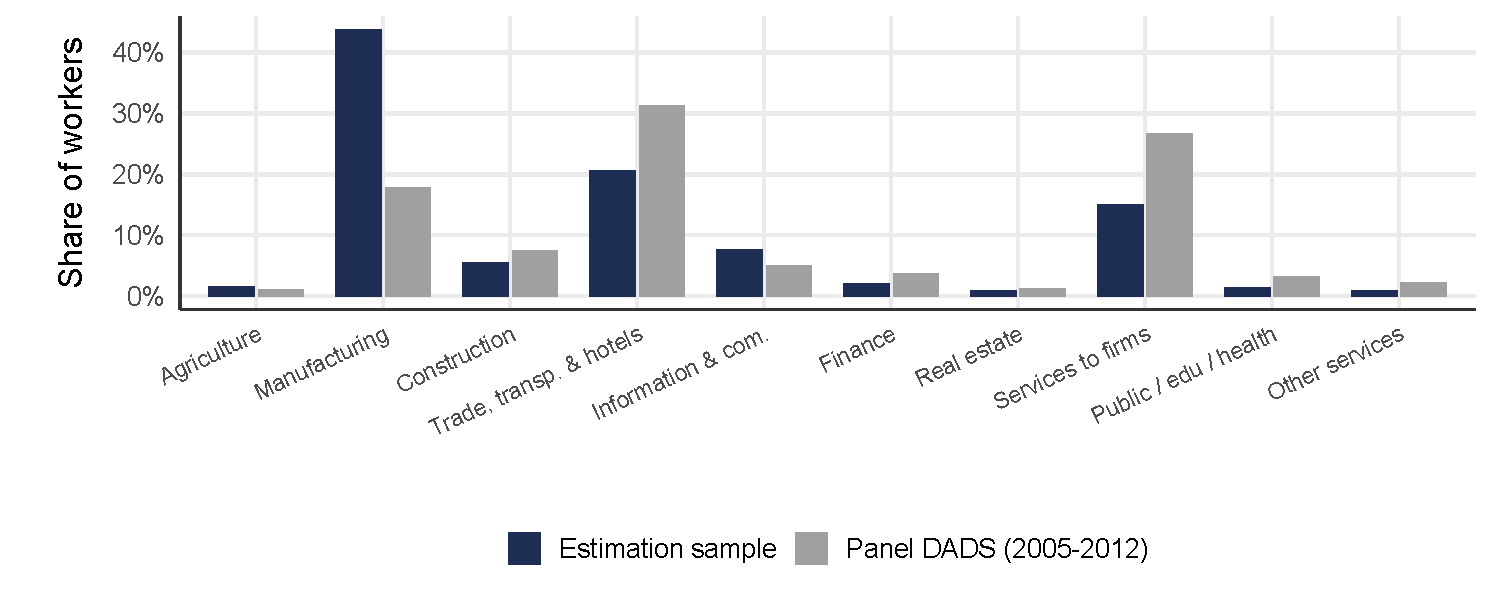
\includegraphics[width=\linewidth, trim={0cm 0cm 0cm 0cm}, clip=true,max width=\linewidth]{figures/02_descriptive_figures/figure_A17_a_mlo_sectors.pdf}
	\end{subfigure}
   
	\begin{subfigure}[b]{\textwidth}
	\caption[]{\small MLO Sample: Occupation\label{fig:desc:MLOocc}}
		\centering
		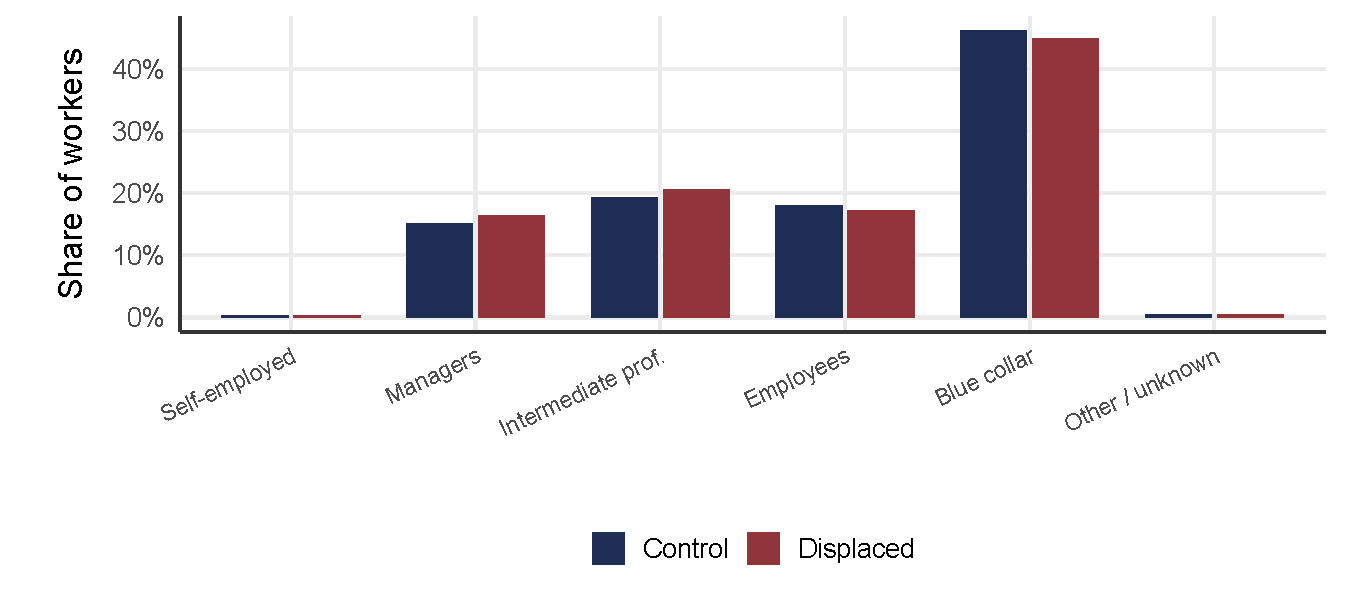
\includegraphics[scale=0.75, trim={0cm 0cm 0cm 0cm}, clip=true,max width=\linewidth]{figures/02_descriptive_figures/figure_A17_b_mlo_occupations.pdf}
	\floatfoot{\footnotesize{\textsc{Notes}: This figure presents descriptive statistics about the sample of 17,949 individuals displaced in a mass layoff (MLO30) and their respective matched controls \textcolor{orange}{[17,946]}. Data is observed at $t^D-1$. Panel (a) reports the distribution of workers across NACE A10 sectors for our \emph{estimation sample} (controls only) and---for reference---the population of private-sector workers in the DADS panel over 2005--2012. We display the control group only because sector is a matching variable, so the MLO-displaced and control-group distributions coincide at $t^D-1$ by construction; controls measured at $t^D-1$ are therefore an accurate description of the sectoral composition of the matched estimation sample. The third bar (Panel DADS) allows the reader to gauge how representative our estimation sample is of the broader French private-sector workforce. Panel (b) displays the distribution of workers across occupations. This variable was not used in the matching algorithm. The sample appears to be balanced across treatment and controls.}}
	\end{subfigure}
\end{figure*}


\clearpage
\section{Robustness: stayer control group\label{app:stayer_controls}}
% Reconstructed from Appendix D of JobDisplacement-3.pdf (pp. 67-69), because
% its separate TeX source was not supplied. Uses the newly generated PDF assets.
In the body of the paper, the control group consists of workers who are never matched
to a displacement event over the sample period; we do not require controls to remain
continuously employed at the same firm over the post-event window. The convention
introduced by \citet{Jacobson1993}\textcolor{orange}{, which \citet{Lachowska2020} also follow,} restricts the control group to ``stayers'' continuously
employed at the same firm; \textcolor{orange}{other} recent contributions \citep{Schmieder2020,bertheau_etal_2023}
do not impose this restriction, and we follow the latter convention. As a robustness
exercise, we re-estimate the main results on the MLO30 sample using a stayer control
group, defined operationally as controls with at least six post-event years of tenure
at the matched firm. The MLO30 sample is the natural locus for this exercise: by
selecting events on a mass-layoff threshold rather than the administrative LE definition,
MLO30 is the closest mapping in our data of the construction adopted in most of the
existing literature, and is therefore the natural sample on which to assess comparability
with the JLS-style stayer convention.

Figure~\ref{fig:stayer:wages} reports the wage decomposition and Figure~\ref{fig:stayer:firms}
reports the firm-level reallocation outcomes, for both control-group definitions.
The substantive contributions of the paper---the firm wage-premium loss, the productivity
gain at destination firms, and the labor-share gap---are essentially unchanged across
the two definitions; the hours and total-earnings scars are mechanically larger under
the stayer control group, because controls subject to any subsequent separation are
excluded from the comparison pool.
\clearpage
\begin{figure}[p]
\centering
\caption{Wage decomposition on the MLO30 sample: baseline (never-displaced) vs. stayer control group}
\label{fig:stayer:wages}
\begin{subfigure}{.74\linewidth}
\caption{Baseline MLO30: never-displaced controls}
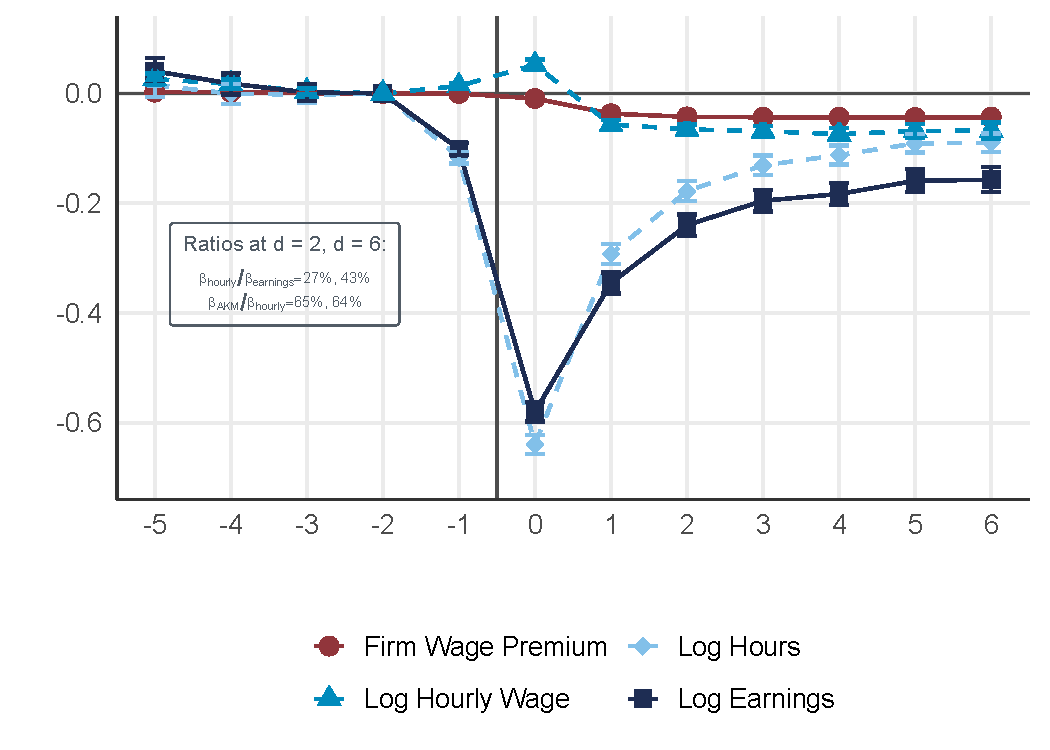
\includegraphics[width=\linewidth,max width=\linewidth]{figures/01_event_figures/figure_A18_a_mlo_baseline_wage_decomposition.pdf}
\end{subfigure}
\par\medskip
\begin{subfigure}{.74\linewidth}
\caption{Stayer MLO30: controls with at least six post-event years of tenure at the matched firm}
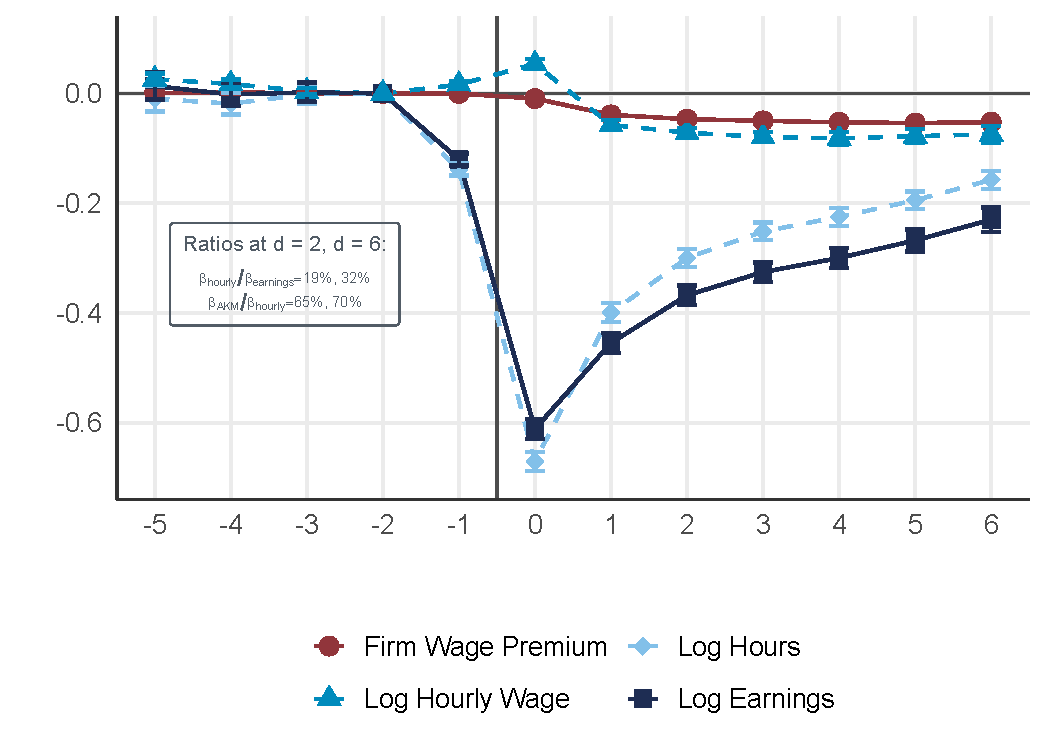
\includegraphics[width=\linewidth,max width=\linewidth]{figures/01_event_figures/figure_A18_b_mlo_stayer_wage_decomposition.pdf}
\end{subfigure}
\floatfoot{\footnotesize\textsc{Notes}: Wage decomposition for the MLO30 sample under two alternative definitions of the control group. Panel (a) uses the baseline never-displaced controls. Panel (b) uses the stayer convention of \citet{Jacobson1993}: controls continuously employed at the same firm over the post-event window. The hourly-wage scar and the firm-wage-premium loss are essentially unchanged across the two definitions; the hours and total-earnings scars are mechanically larger under the stayer convention. Standard errors: robust standard errors clustered at the worker level; displayed confidence intervals at the 99\% level.}
\end{figure}
\clearpage
\begin{figure}[p]
\centering
\caption{Productivity, labor share and firm wage premium of current employers on the MLO30 sample: baseline vs. stayer control group}
\label{fig:stayer:firms}
\begin{subfigure}{\linewidth}
\caption{Baseline MLO30: never-displaced controls}
\begin{tabular}{ccc}
Productivity & Labor share & Firm wage premium\\
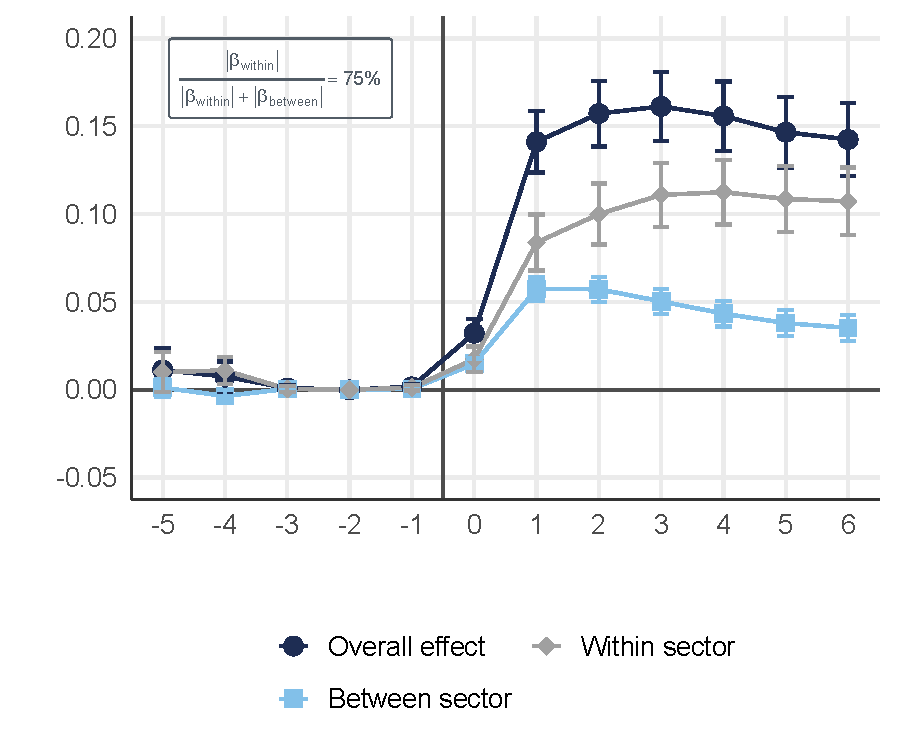
\includegraphics[width=.30\linewidth,max width=\linewidth]{figures/01_event_figures/figure_A19_a_baseline_productivity.pdf}&
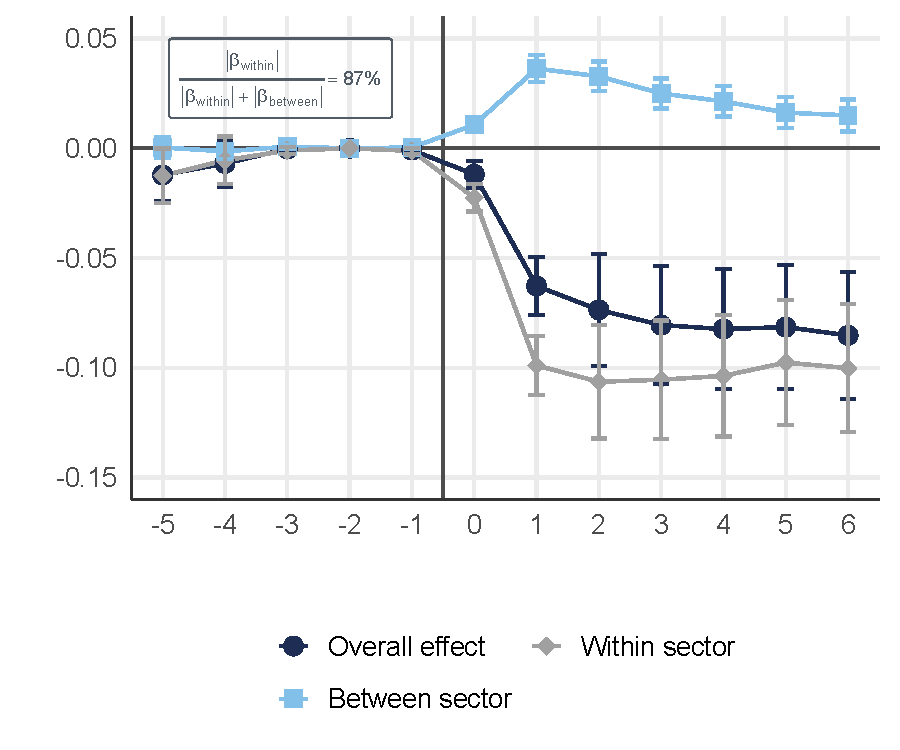
\includegraphics[width=.30\linewidth,max width=\linewidth]{figures/01_event_figures/figure_A19_a_baseline_labor_share.pdf}&
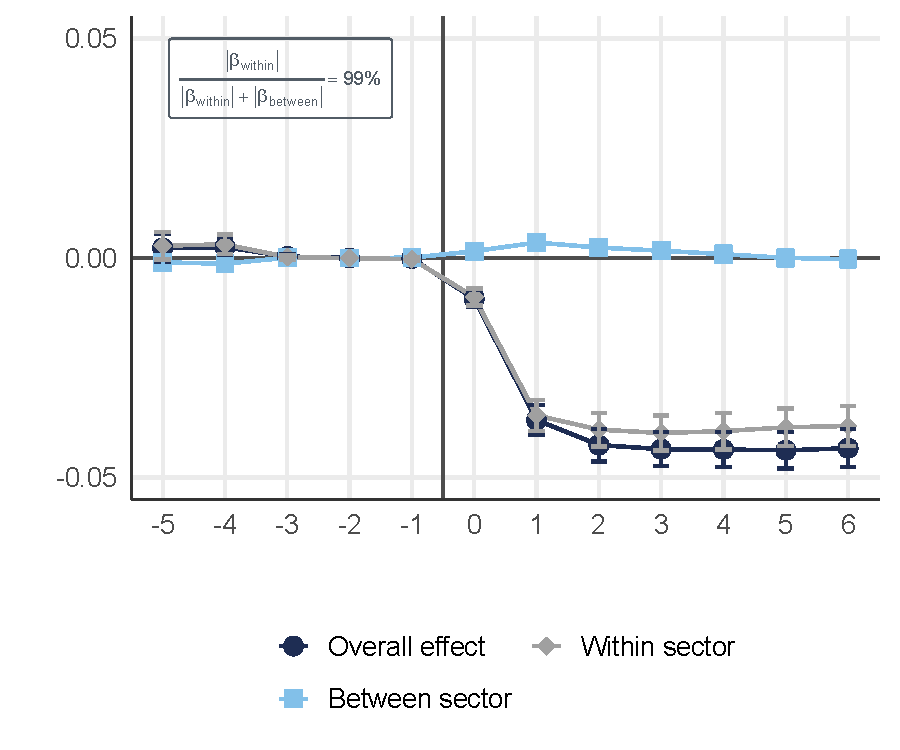
\includegraphics[width=.30\linewidth,max width=\linewidth]{figures/01_event_figures/figure_A19_a_baseline_firm_premium.pdf}
\end{tabular}
\end{subfigure}
\par\medskip
\begin{subfigure}{\linewidth}
\caption{Stayer MLO30: controls with at least six post-event years of tenure at the matched firm}
\begin{tabular}{ccc}
Productivity & Labor share & Firm wage premium\\
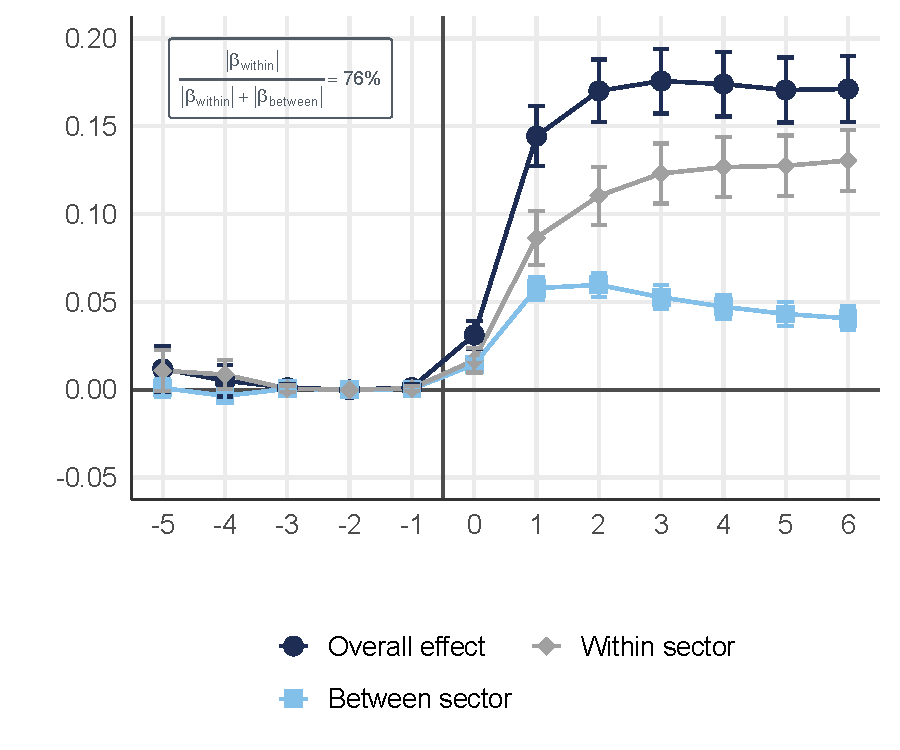
\includegraphics[width=.30\linewidth,max width=\linewidth]{figures/01_event_figures/figure_A19_b_stayer_productivity.pdf}&
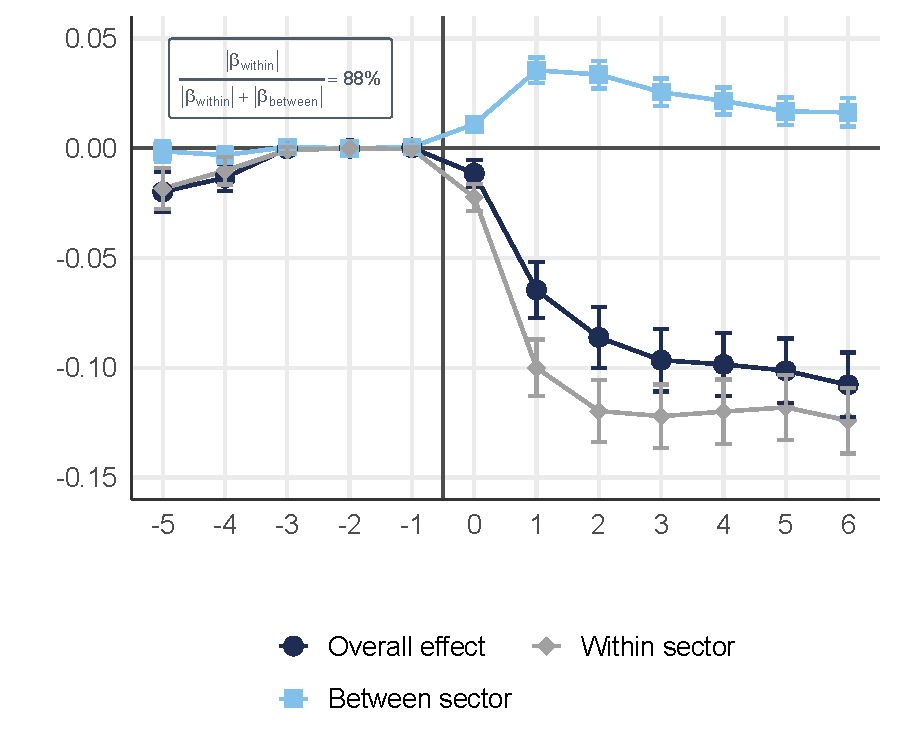
\includegraphics[width=.30\linewidth,max width=\linewidth]{figures/01_event_figures/figure_A19_b_stayer_labor_share.pdf}&
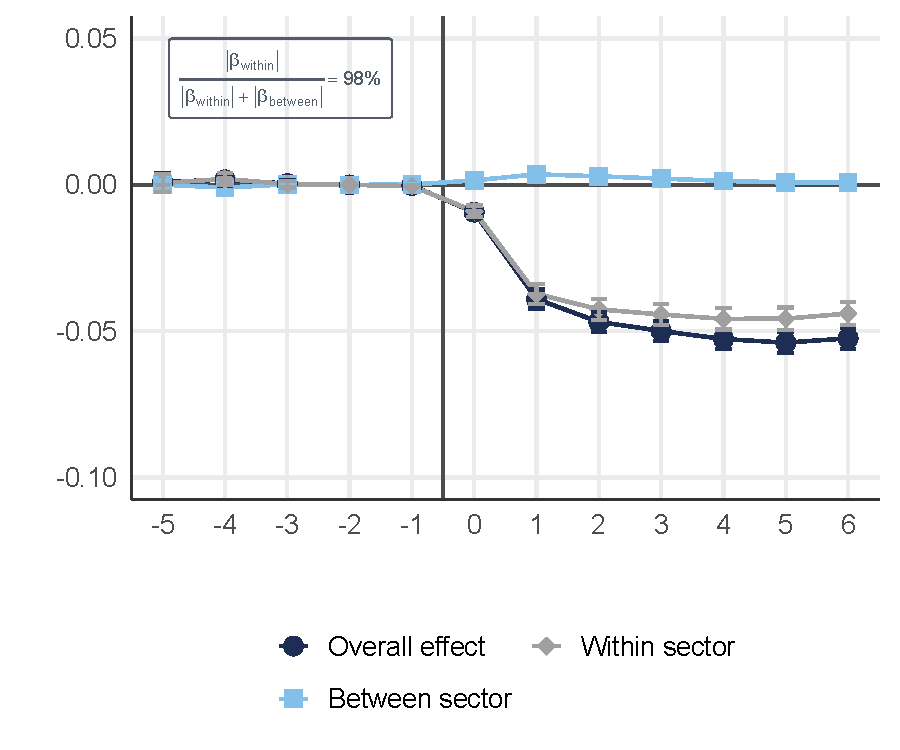
\includegraphics[width=.30\linewidth,max width=\linewidth]{figures/01_event_figures/figure_A19_b_stayer_firm_premium.pdf}
\end{tabular}
\end{subfigure}
\floatfoot{\footnotesize\textsc{Notes}: Firm-level reallocation outcomes (productivity, labor share, AKM firm wage premium of current employers) for the MLO30 sample under two alternative definitions of the control group. Panel (a) uses the baseline never-displaced controls. Panel (b) uses the stayer convention of \citet{Jacobson1993}. Standard errors: robust standard errors clustered at the worker level; displayed confidence intervals at the 99\% level.}
\end{figure}
\clearpage


\clearpage
\section{Negotiation\label{appsec:nego}}
%%%%%%%%%%%%%%%%%%%%%%%%%%%%%%%%%%%%%%%%%%%%%%%%%%%%%%%%%%%%%%%%%%%%%%%%%%%%%%%
%                                                                             %
% Cette version repart de 03_Draft\appendix\appendix_negotiations_current.tex %
%                                                                             %
%%%%%%%%%%%%%%%%%%%%%%%%%%%%%%%%%%%%%%%%%%%%%%%%%%%%%%%%%%%%%%%%%%%%%%%%%%%%%%%

In section \ref{sec:Nego} of the paper, we investigate the link between displacement and change in firm-level negotiations characteristics, making use of two administrative data sets that provide firm-level characteristics relative to workplace negotiations. We provide more detail on the data used. The first data gives detailed information about collective agreements signed (or discussed) within firms. The second data measures turnout and results from workplace elections. These two data sets provide rare and direct insight into in-house bargaining, a potential mechanism underlying the loss in firm-level wage premia experienced by displaced workers. In this online appendix section, we first present the collective agreements data in subsection \ref{appsec:accord_data} and the election data in subsection \ref{appsec:elec_data}. In subsection \ref{appsec:robust_samples} we show that the sample restrictions we make for this analysis do not affect our main conclusions. Finally, in subsection \ref{appsec:neg:results} we display more detailed results, complementing the analysis presented in the main text. 

\subsection{Collective agreements\label{appsec:accord_data}}

% https://www.service-public.fr/professionnels-entreprises/vosdroits/F31400

In order to document the number and type of collective agreements signed by firms, we use the ``D@ccord'' data set, produced by the Ministry of Labor research and statistics direction (DARES), and available since 2005. The French labor law requires firm-level collective agreements to be filed on a dedicated online platform. Each negotiation has to be reported, even when no agreement is reached. The D@ccord data contains information on the type of reported text, be it an actual firm-level collective agreement, or a report of disagreement. It also provides information on the matter of the negotiations (e.g. wages, hours, layoffs, etc.), on the parties negotiating or signing the agreement, the date of signature of the agreement, and the firm identifier (SIREN), which we use to match this data with our main samples (LE or MLO).

The D@ccord data enables us to build several variables describing the type, number and subject of collective agreements signed each year in a given firm. We consider 3 main bargaining subjects: agreements on wages and bonuses; agreements related to earnings more generally (wages and bonuses, ranking,\footnote{Within a firm, a worker's ranking (\textit{classification} in French) is used to determine the position, duties and minimum wage applicable to the employee.} profit-sharing and participation); agreements related to hours and working time.

Our main measure of collective agreement is an indicator taking value 1 if a firm has signed (at least) one agreement relative to earnings (i.e. type 1.) over the 2005-2007 period, and 0 otherwise. We assign 0 to firm for which we do not observe any agreements (our results are robust to excluding those) -> (\textcolor{red}{this is the old definition, we have the that the firm has to have operated during 2005-2007 and has at least 50 workers}) \textcolor{orange}{[proposed: ``The sample is restricted to firms that operated over 2005--2007 and had at least 50 employees; firms for which no agreement is observed are assigned 0 (our results are robust to excluding them).'']}. Alternatively, we consider a continuous version of the outcome, summing all the observed agreements on earnings over the period (and assigning 0 to other firms). Next, we consider failed negotiations about the same topic; that is negotiations that yield no signed agreement. Finally, we also consider indicators for the signature of (at least) one agreement of each of the other types separately. 

Table \ref{tab:nego:LEnego_acc_desc} describes the distribution of those outcomes in our sample of analysis. About 61.5\% of firms employing individuals in our sample \textcolor{orange}{[24.6\%: Table~\ref{tab:nego:LEnego_acc_desc}, mean 0.246]} have signed (at least) one agreement about wages over 2005-2007. This leads to an average number of 2.27 agreements \textcolor{orange}{[0.89]} signed by those firms over the period. At the same time, 26.9\% also failed to sign \textcolor{orange}{[10.4\%]} a wage agreement they had started to negotiate. Finally, 53.2\% signed an agreement on working time and hours \textcolor{orange}{[21.1\%]}.


% Est-ce qu'on dit participation en anglais ? ou les 2 (participation et intéressement) vont dans "profit sharing" ?

% L'intéressement est un dispositif d'épargne salariale lié aux résultats ou aux performances de l'entreprise. Toutes les entreprises peuvent le mettre en place, par voie d'accord avec les salariés. Le bénéficiaire de l'intéressement perçoit une prime dont le montant et les conditions de versement sont fixés par l'accord d'entreprise. Les sommes sont immédiatement disponibles, mais le salarié peut choisir de les placer sur un plan d'épargne salariale ou un compte épargne-temps.

% La participation est un mécanisme de redistribution des bénéfices de l'entreprise aux salariés. Elle est obligatoire dans les entreprises dont l'effectif est de 50 salariés ou plus. Le salarié bénéficiaire reçoit une prime dont le montant est fixé par l'accord de participation. Il peut demander le versement immédiat des sommes ou leur placement en épargne. Dans ce cas, les sommes sont indisponibles pendant 5 ans. L'accord de participation précise comment les sommes sont placées.

% 1. Salaires et primes (OBJN1)
% 2. Salaires et primes (OBJN1), Classifications (OBJN2), Intéressement (OBJN3), Participation (OBJN4)
% 3. Accords de méthode (PSE) (OBJN15), Accès et maintien des salariés dans l'emploi (OBJN16)
% 4. Durée collective temps de travail (anciennement RTT) (OBJN9), Aménagement du temps de travail (OBJN10), CET (OBJN11), Fixation des congés (anciennement "modulation") (OBJN11), Heures supplémentaires (OBJN34), Travail du dimanche (OBJN36)


\begin{table}[h]
\caption{Collective agreements outcomes, descriptive statistics}
\begin{center}
\label{tab:nego:LEnego_acc_desc}
\begin{adjustbox}{max width=\linewidth}
\begin{tabular}{l|lllllll}\toprule
% Generated from current results_analysis CSV files by master.R, section I (scripts/I-PLOTS_AND_TABLES).
% Table A16; status: ready
% Sample: le5_panelsize0-acco_alt. N counts nonmissing observations for each outcome; the treated count describes the full sample. Agreement outcomes cover 2005-2007; uses exported p75.
% -- means a requested statistic is unavailable; an empty cell means not applicable.
 & Mean & sd & min & p75 & max & $N$ \\
\hline
Wage agreement indicator & 0.541 & 0.498 & 0 & 1 & 1 & 90,120 \\
\# Wage agreement & 1.984 & 3.541 & 0 & 3 & 52 & 90,120 \\
Wage failure ind. & 0.232 & 0.422 & 0 & 0 & 1 & 90,120 \\
Hours agreement ind. & 0.466 & 0.499 & 0 & 1 & 1 & 90,120 \\
\hline
\# Treated (sample) & 16,512 &  &  &  &  &  \\

\bottomrule
\end{tabular}
\end{adjustbox}
\floatfoot{{\footnotesize \textsc{Notes}: This table provides simple descriptive statistics about collective agreements outcomes. \textbf{Sample}: The sample of interest is all workers laid-off for economic reason (LE) after 2007, and their respective controls. \textbf{Outcomes}: Table \ref{apptab:definitions} summarizes variables' definition. Wage agreement indicator takes value 1 if the firm has signed (at least) one agreement relative to wages, and 0 otherwise. \# Wage agreement is the number of wages agreement signed by the firm. Wage failure indicator takes value 1 if the firm has failed to conclude (at least) one negotiation relative to wages. Hours agreement indicator takes value 1 if the firm has signed (at least) one agreement relative to hours and working time.}}

\end{center}
\end{table}



% SAMPLE RESTRICTION
We use the collective agreements outcome to explore the evolution of firm-level characteristics (relative to negotiation) for displaced workers. Because the data starts in 2005 (i.e. after the first layoff we observe), one may worry about potential reverse causality. This would be the case if firm-level negotiations happen right after a layoff and respond to it. To limit this risk as much as possible, we focus our analysis on a sub-sample of displaced workers for which we can measure firm-level negotiations strictly before the layoff. In practice, we only consider workers affected by a layoff after 2007 while, at the same time, we construct firm outcomes over the 2005-2007 period only. In subsection \ref{appsec:robust_samples} below, we show that this sub-sample resembles our main sample of analysis and that our main results hold true.



 


\FloatBarrier
\subsection{Workplace elections\label{appsec:elec_data}}
We next observe workplace elections. Our data covers the 2009 to 2012 period and provides detailed measures on many elections (number of electors, number of voters, results by trade union, etc.). Workplace elections in France are very heterogeneous. This is because, within a common legal framework, each firm can set the exact format of its elections. Below, we briefly detail the main legal framework as well as the data we observe. In a nutshell, we use a firm-level measure of turnout at the elections as an indication of within-firm quality of negotiations.


\paragraph{Main legal framework}
In France (and over the period of interest), workers elect representatives at most every 4 years. Those representatives are elected for three distinct (but complementary) bodies:
\begin{itemize}
\item[-] The DP (for ``Délégué du Personnel'') in firms with 11 employees or more.

\item[-] The CE (for ``Comité d'Entreprise'') in firms with 50 employees or more. In those firms, CE and DP elections take place at the same time. Elected representatives can be member of the two bodies at the same time.

\item[-] The DUP (for ``Délégué Unique du Personnel'') can be elected in firms with 50 to 299 employees. They are meant to ease the negotiation by merging the three main bodies of workers' representation (the aforementioned DP and CE, and the ``CHSCT'' a third committee in charge of health and safety and whose member are designated by DP or CE).
\end{itemize}


\paragraph{Elections in practice}
%In practice, elections take place in a $Year \times Body \times Level \times Occupation$ stratum. The $Year$ is at most every four years, but partial elections can be organized if needed (i.e. when a representative and her substitute have to be replaced). The $Body$ is either DP, CE and/or DUP. The $Level$ can be either the firm or each establishment. And the $Occupation$ means that different occupations (e.g. blue collars, technicians or high-skilled professionals) can organize distinct elections. The exact stratum is actually defined differently in each firm, through internal negotiations prior to the election. To keep the simplest information here we: i) ignore partial elections and ii) aggregate the data at the firm level (weighting each $Body \times Level \times Occupation$ by its number of electors, when needed). That allows us to obtain one observation per firm, (at most) every 4 years. 

Within this main framework, each firm has the ability to decide about how the election is to be organized in practice. That is, prior to an election, within-firm negotiation will decide about strata in which (sub-)elections are organized. The choices relate to:
\begin{itemize}
\item[-] The body $b$ of the election. As explained before, depending on firm size, elections may take place to elect either DP and/or CE and/or DUP.
\item[-] The year $y$ of the election. Although every 4 years is legally binding, some firm may have to organize elections more often due to sector agreements or because a representative (and her substitute) has to be replaced in a partial elections. In our analysis, we ignore partial elections.\footnote{Election can have more than one round, but we focus our analysis on first round only. This is because the second round only takes place when the election fails either because i) no trade union ran for the election or ii) less than 50\% of electors voted. As explained below, we do take into account this type of failure.}
\item[-] The level $l$ which can be either the entire firm or its establishment separately.
\item[-] The occupation $o$ meaning that different types of workers (e.g. blue collars, engineers, etc.) can decide to vote in distinct elections.
\end{itemize}

Importantly, each firm will decide of a stratum defined by $b \times y \times l \times o$. For instance, one firm may have only one single election for all its workers (regardless of their establishments and occupation) to elect representative in DP and CE body; whereas another firm may organize election at the establishment-level, with each establishment following its own calendar (e.g. 2009-2013 for one, 2010-2014 for another, etc.). Given the number of possible options, there is substantial heterogeneity in size and timing of elections.

\paragraph{Data cleaning and outcomes definition} To ease the analysis, we collapse each election result at the firm times body (i.e. DP, CE, or DUP -- $b$) level. That is, we ignore the divisions in $l$, $o$ and $y$. Summing numbers across $l$ and $o$ is straightforward as those categories are exclusive (i.e. one worker belongs to one single establishment  and one single occupation). We decide to ignore years $y$ for two reasons. First because our data does not allow us to know whether different years simply reflect internal organization of the election (e.g. different establishments voting on different dates) or occurrence of main elections at less than 4 years interval. Second, over the 2009-2012 period, most firms (80\%) are observed in only 1 year. To aggregate information at the firm times body level, we weight each stratum by its number of electors. 

This simplification allows us to construct three main outcomes. First, we observe the average election turnout for the observed firms over the 2009-2012 period. This outcome is the average participation across the different bodies $b$ (i.e. between 1 and 3 distinct elections) of a given firm. We complement this main outcome with two others. The second outcome we compute is the share of workers who are covered by an election that failed;\footnote{An election fails if no trade union ran for the election.} where we think of election failure as an indication of a low quality of workplace negotiation. Finally, our third outcome is the share of workers who are covered by an election where a CGT representative received more than 10\% of the votes;\footnote{The 10\% threshold is important as it allows a candidate to become ``Délégué Syndicale'' or DS -- not DP --, who take part in negotiations about wages. This threshold is measured in the first round of the election.} where we think of CGT as indicating more conflictual negotiation. The CGT is one of the oldest (1895) and main trade union in France, traditionally seen as left-oriented (with marxist origins). A small literature also finds CGT union to be associated with higher wages \citep{abowd_persistent_2012, breda_firms_2015}. This renders the meaning of the CGT outcome more complex and suggests cautious interpration.

Table \ref{tab:nego:LEnego_ele_desc} describes the empirical distribution of those outcomes in the firms of our sample of analysis (cf. below about the sample). The workers in our sample are employed by firms that had an average turnout of 64.3\% \textcolor{orange}{[59.6\%: Table~\ref{tab:nego:LEnego_ele_desc}, mean 0.596]} at professional elections held over 2009-2012. On average in those firms, about 11.6\% of the workers were affected by failed election \textcolor{orange}{[22.4\%]}. Finally, about 50\% of the workers \textcolor{orange}{[OK: 50.4\%]} were involved in an election where a CGT candidate had received 10\% or more of the votes.

%A propos de 

%\iffalse 

%\begin{table}[h] 
%\caption{Elections sample}
%\begin{center}
%\input{03_Draft/tables/desc_nego_LE_elections.tex}  %\label{tab:nego:desc_nego_LE_elections}
%\floatfoot{{\footnotesize \textsc{Notes}: ...}} 
%\end{center}
%\end{table}

%\fi

%We are mainly interested in two dimensions of the election outcome: the turnout, and the vote for CGT. We consider turnout as an indicator of work relations within the firm. We next build an indicator taking the value 1 if the CGT union had a candidate in the election, and 0 otherwise. CGT is one of the oldest and most important Union in France (???) but is often regarded as more conflictual (???, SOURCE?). We view the presence of CGT as an indicator of ???.



\begin{table}[h]
	\caption{Elections outcomes, descriptive statistics}
	\begin{center}
		\label{tab:nego:LEnego_ele_desc}
		\begin{adjustbox}{max width=\linewidth}
\begin{tabular}{l|lllllll}\toprule
			% Generated from current results_analysis CSV files by master.R, section I (scripts/I-PLOTS_AND_TABLES).
% Table A17; status: ready
% Sample: le5_panelsize0-election. N counts nonmissing observations for each outcome; the treated count describes the full sample. Election outcomes cover 2009-2012; uses exported p50. Failed = no-candidate share, not blank votes.
% -- means a requested statistic is unavailable; an empty cell means not applicable.
 & Mean & sd & min & p50 & max & $N$ \\
\hline
Average turnout & 0.610 & 0.262 & 0 & 0.695 & 1.000 & 90,252 \\
Failed (\% workers) & 0.200 & 0.377 & 0 & 0.000 & 1.000 & 104,412 \\
CGT (\% workers) & 0.515 & 0.391 & 0 & 0.622 & 1.000 & 94,442 \\
\hline
\# Treated (sample) & 17,071 &  &  &  &  &  \\

			\bottomrule
		\end{tabular}
\end{adjustbox}
		

		\floatfoot{{\footnotesize \textsc{Notes}: This table provides simple descriptive statistics about professional election outcomes. \textbf{Sample}: The sample of interest is all workers laid-off for economic reason (LE), and their respective controls, whose firm have at least one election between 2009-2012 (observed in the data). \textbf{Outcomes}: Table \ref{apptab:definitions} summarizes variables' definition. Average turnout is the worker-weighted average participation of electors in firm-specific professional elections. See details in \ref{appsec:elec_data}. Failed is the share of firm's workers who were electors for a (eventually) failed election (i.e. no trade union ran). CGT is the share of firm's workers who were electors in an election were a CGT representative received more than 10\% of the votes.}} 
	\end{center}
\end{table}



Our data of workplace elections covers the end of our period of analysis (2009-2012). This timing is problematic because the majority of the layoffs we observe take place before. To limit the risk of reverse causality, we take advantage of our LE setting, where small (even individual) layoffs can be observed. In particular, we verify that our election results are robust to considering only a sub-sample of layoffs were the number of displaced workers is small, relative to the firm size. In our sample, this means considering layoffs affecting 6.7\% (\textcolor{red}{where does the number come from? to be removed}) \textcolor{orange}{[agreed: the 6.7\% cannot be traced to any table; drop it]} of firms' employees or less (the lowest 25\% in our sample -> \textcolor{red}{lowest quartile of the observed layoff-share measure in the election sample}).%\footnote{In the sample, 25\% of LE workers are observed along 0.56\% of their own firm' workforce. Given that we observe a 1/12 sample of workers, this represent about 6.7\% of firm's employees.}
 This robustness test addresses the risk that the relative decline in employers' average turnout result from an actual increase in previous employers' turnout (e.g. if workers vote more after a lay-off affected their colleagues) than a re-employment mechanism.



\FloatBarrier
\subsection{Robustness of the main results \label{appsec:robust_samples}}
The sample we use to perform analysis on collective agreements and elections differ from our main sample of analysis. In the case of collective agreements, this is because we consider only those workers who lost their job from 2008. In the case of electoral results, this is because we do not observe the universe of firms. Although we tried to follow transparent rules, nothing entirely prevents the selection of specific sub-samples. In this subsection, we show that these selections do not alter the sample observable characteristics too much and that our main results on labor (earnings, hours worked, wage rates and premia) %and firm (productivity, value added per worker, labor share, size) 
holds across samples.

Figure \ref{fig:neg:roblabor} below reproduce Figure \ref{fig:fe_current_event_mlo_pretrends} for the two sample we use when estimating effects in accords and elections outcomes. 

%XXX TO BE COMPLETED, GRAPHS READY: LE\_accords\_age\_robfirm \\
%or LE\_elections\_lnsize\_roblabor, etc.


\begin{figure}[h!] \centering
	\caption{Loss in wage premia for accords and election samples} \label{fig:neg:roblabor}
	\begin{subfigure}[b]{\textwidth}
		\centering
		\caption[]{\small Accords sample \label{fig:neg:roblabor:acc}}
		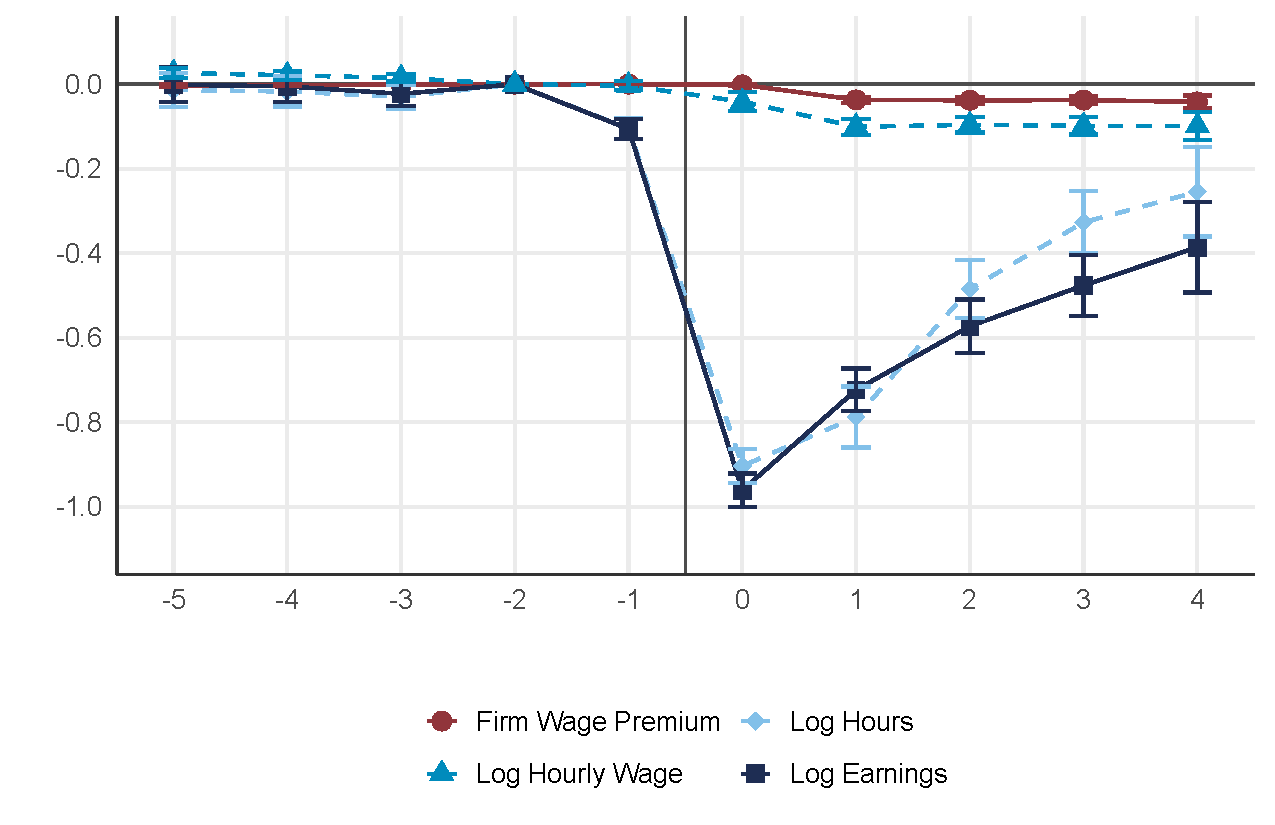
\includegraphics[width=.79\linewidth,max width=.79\linewidth]{figures/01_event_figures/figure_A20_a_agreements_sample.pdf}
	\end{subfigure}

	\begin{subfigure}[b]{\textwidth}
		\centering
		\caption[]{\small Election sample \label{fig:neg:roblabor:elec}}
		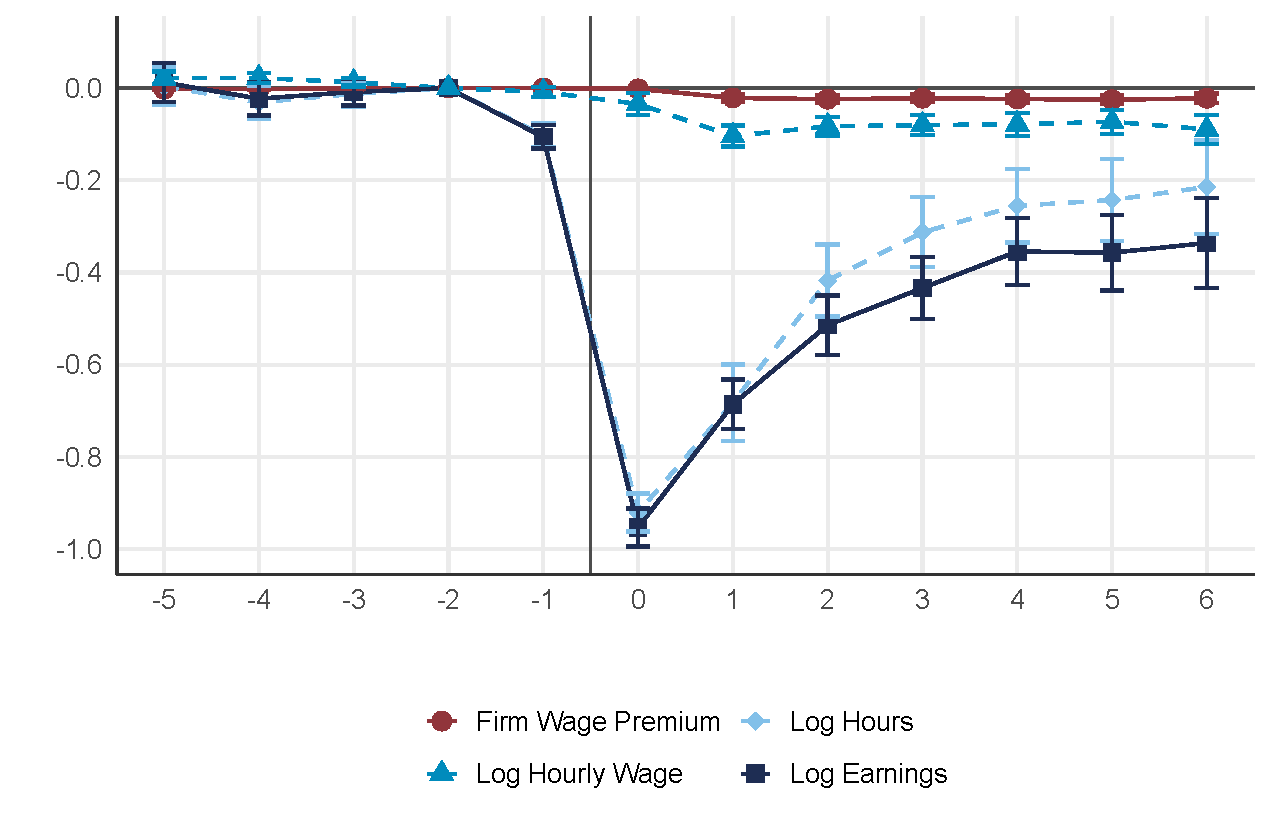
\includegraphics[width=.79\linewidth,max width=.79\linewidth]{figures/01_event_figures/figure_A20_b_elections_sample.pdf}
	\end{subfigure}
	
	\floatfoot{\footnotesize{\textsc{Notes}: This figure reports event-study estimates of the cost of job displacement on four outcomes (log hourly wage, log hours, log earnings, and the AKM firm wage premia) for the two LE sub-samples used in the negotiation analysis. Outcomes are all expressed in log points; frim wage premia correspond to the contamination-corrected AKM firm fixed effects. \textbf{Samples}: our data on collective agreements and professional elections require us to work on sub-samples. Panel~(a) (accords sample) is estimated on workers laid-off after 2007 and is therefore restricted to $d \leq 4$. Panel~(b) (election sample) is estimated on workers for whom we obtain firm-level election data and extends to $d=+6$. \textbf{Definition of the outcomes}: Table~\ref{apptab:definitions} summarizes variables' definition. \textbf{Standard errors}: robust standard errors clustered at the worker level; displayed confidence intervals at the 99\% level.}}
\end{figure}



\FloatBarrier
\subsection{Results on negotiation outcomes}\label{appsec:neg:results}

\paragraph{Collective agreements}
Table \ref{tab:nego:LEnego_acc_result} presents our main results on collective agreements outcomes. Destination firms were less likely to have signed any wage-related agreement over the 2005-2007 period (column (1)). By $t+4$ the average displaced worker finds himself in a firm that is 7.8 percentage points less likely (than his previous firm) \textcolor{orange}{[5.9: Table~\ref{tab:nego:LEnego_acc_result}, col. 1 at $t+4$ = $-0.059$]} to have signed a wage-setting agreement. Column (2) shows a qualitatively similar finding when considering a continuous version of the same outcome (total number of agreements) instead of the indicator: destination firms have signed about 0.33 fewer wage agreements \textcolor{orange}{[0.29: $-0.287$]} than origin firms by $t+4$. Column (3) shows that destination firms are also relatively more likely to fail to sign agreements (a $+8.3$ percentage-point gap by $t+4$) \textcolor{orange}{[$+8.0$: 0.080]}. This result suggests that the difference between origin and destination firms is not merely quantitative but also has a qualitative component to it. Finally column (4) reports the result for having at least one agreement related to working time: destination firms are 11.3 percentage points less likely \textcolor{orange}{[12.2: $-0.122$]} to have signed such an agreement by $t+4$.


Firm size positively correlates with collective agreements. One could therefore fear that the main results on collective agreements only reflect the change in employer's size we found. Of course, if this was the case, the role of negotiation would still be meaningful in its own right. However, showing that the loss in negotiation holds even when controlling for employers' size is a stronger result as it suggest that size and negotiation have different (complementary) effects. In Table \ref{tab:nego:LEnego_acc_rob} we show that controlling for (log) size (column (2)) only increases the loss in employers' probability to have had an agreement signed. Further, in column (3) we also include fixed effects for four size categories (from 0 to 10, from 11 to 49, from 50 to 299 and above 299 employees) defined so as to follow legally relevant threshold (e.g. ``DP'' being elected above 10 employees; ``CE'' being required above 50, etc.). The results remain virtually the same. 


\paragraph{Elections}
Table \ref{tab:nego:LEnego_ele_result} presents our main results on elections outcomes. We observe that destination firms had lower average turnout over the 2009-2012 elections round (column (1)). By $t+5$, the displaced workers' new employer has a 14pp. lower turnout (relative to previous employer). Beyond turnout, we also find that hiring firms are also relatively more likely to have failed elections on the one hand (column (2)) or CGT candidates succeeding at the 10\% threshold (column (3)). All three outcomes indicate that the hiring firm face more complicated in-house negotiations. In Table \ref{tab:nego:LEnego_ele_rob} we further show that the result on the turnout outcome remains true when controlling for (log) size; or when considering a sub-sample of lay-offs that were small relative to the firm size. In both cases, the qualitative result holds; confirming that displaced individuals join firms with relatively lower turnout at workplace elections. The last result (column (3) of Table \ref{tab:nego:LEnego_ele_rob}) also suggest that the observed turnout is not driven by an endogenous reply to lay-off (in former employers' turnout).
 

\begin{table}[h] 
	\caption{Agreements results} \label{tab:nego:LEnego_acc_result}
\begin{center}
{\footnotesize\begin{adjustbox}{max width=\linewidth}
\begin{tabular}{l|llll}\toprule
	% Generated from current results_analysis CSV files by master.R, section I (scripts/I-PLOTS_AND_TABLES).
% Table A18; status: ready
% 
% -- means a requested statistic is unavailable; an empty cell means not applicable.
 & (1) & (2) & (3) & (4) \\
Time to displ. & Wage agree. ind. & \# Wage agree. & Wage fail. ind. & Hours agree. ind. \\
\midrule
$d=-3$ & 0.018 & 0.050 & 0.017 & 0.011 \\
 & (0.003) & (0.015) & (0.003) & (0.003) \\
$d=-2$ & REF & REF & REF & REF \\
 &  &  &  &  \\
$d=-1$ & -0.000 & 0.005 & -0.000 & -0.000 \\
 & (0.001) & (0.004) & (0.001) & (0.001) \\
$d=0$ & -0.014 & -0.049 & 0.028 & -0.021 \\
 & (0.004) & (0.020) & (0.003) & (0.004) \\
$d=1$ & -0.061 & -0.572 & 0.134 & -0.144 \\
 & (0.013) & (0.084) & (0.012) & (0.013) \\
$d=2$ & -0.059 & -0.542 & 0.102 & -0.135 \\
 & (0.014) & (0.091) & (0.013) & (0.014) \\
$d=3$ & -0.071 & -0.505 & 0.074 & -0.123 \\
 & (0.016) & (0.103) & (0.014) & (0.016) \\
$d=4$ & -0.059 & -0.287 & 0.080 & -0.122 \\
 & (0.022) & (0.162) & (0.019) & (0.023) \\
\midrule
Individuals & 28,198 & 28,198 & 28,198 & 28,198 \\
\# treated & 16,597 & 16,597 & 16,597 & 16,597 \\

	\bottomrule
\end{tabular}
\end{adjustbox}}
		\floatfoot{{\footnotesize \textsc{Notes}: This table presents event-study estimates of the reallocation of workers displaced for economic reason (LE) across firms with different approach to collective agreement ---see equation (\ref{eq:main_estimating_equation}) and associated text for more details on the specification. \textbf{Comment on timing}: Firm-level outcomes are computed over the 2005-2007 period. To limit the risk of reverse causality we restrict our sample to individuals displaced after 2007. We thus do not observe individuals after $t^D+4$. Accordingly, event-study coefficients reflect the movement of displaced workers to firms with different initial characteristics and \textit{not} changes within-firm in such characteristics. \textbf{Outcomes}: Table \ref{apptab:definitions} summarizes variables' definition. Wage agreement indicator is an indicator taking value 1 if the firm has signed (at least) one agreement relative to wages over the period. \# Wage agreement is the number of wages agreement signed by the firm. Wage failure is an indicator taking value 1 if the firm has failed to conclude (at least) one negotiation relative to wages. Hours agreement indicator takes value 1 if the firm has signed an agreement relative to hours or working time. Details about those outcomes are given in \ref{appsec:accord_data}. \textbf{Standard errors}: robust standard errors clustered at the worker-level.}}
\end{center}
\end{table}


\begin{figure}[h!]
	\centering
	\caption{Event-study coefficients for the agreement outcomes of Table~\ref{tab:nego:LEnego_acc_result}}\label{fig:nego:LEnego_acc_evstudy}
	\begin{subfigure}[b]{.49\textwidth}
		\centering
		\caption[]{\small Wage agreement indicator (column~1)} \label{fig:nego:wage_ind}
		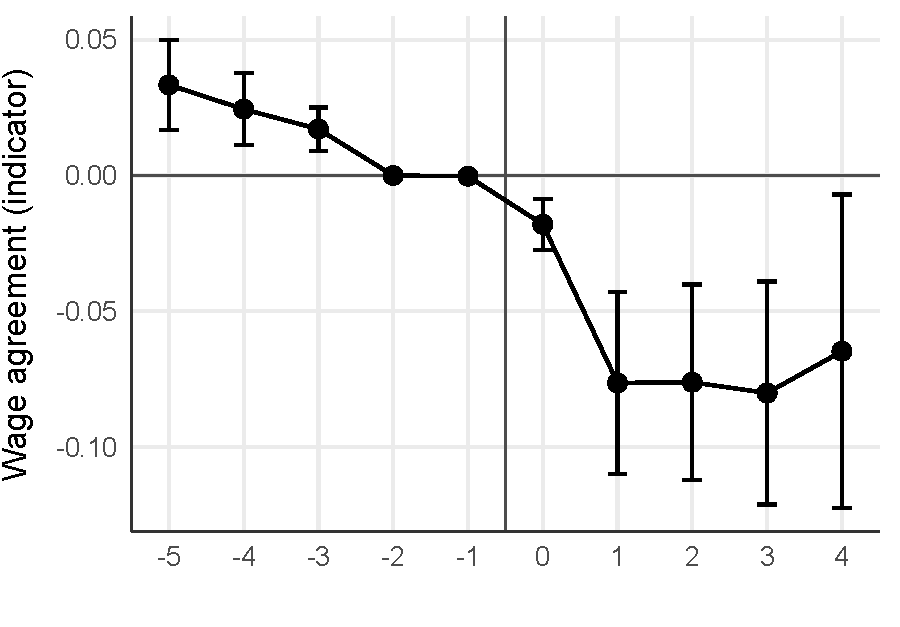
\includegraphics[width=\linewidth,max width=\linewidth]{figures/01_event_figures/figure_A21_a_wage_indicator.pdf}
	\end{subfigure}
	\begin{subfigure}[b]{.49\textwidth}
		\centering
		\caption[]{\small \# wage agreements (column~2)} \label{fig:nego:wage_num}
		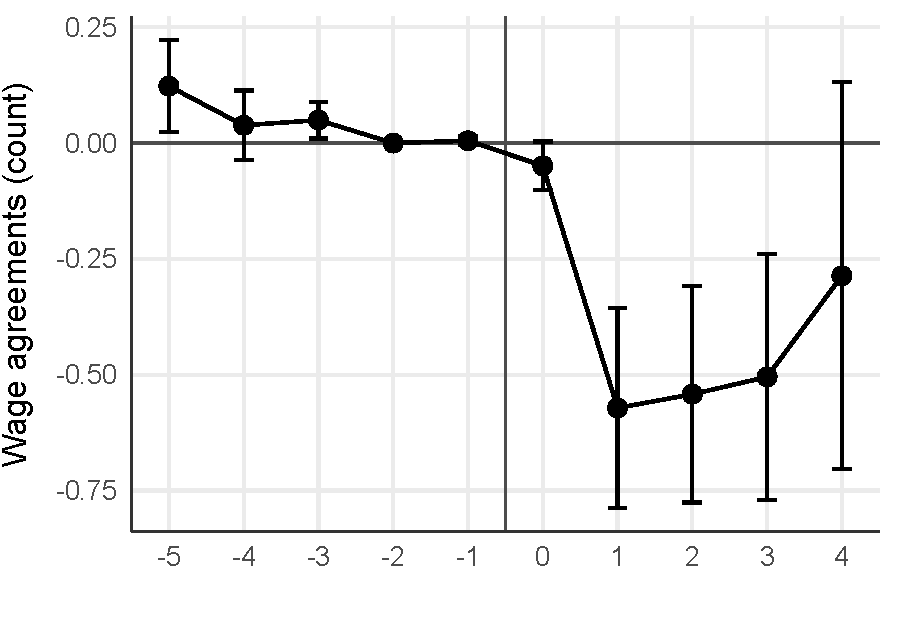
\includegraphics[width=\linewidth,max width=\linewidth]{figures/01_event_figures/figure_A21_b_wage_count.pdf}
	\end{subfigure}

	\begin{subfigure}[b]{.49\textwidth}
		\centering
		\caption[]{\small Hours agreement indicator (column~4)} \label{fig:nego:hours_ind}
		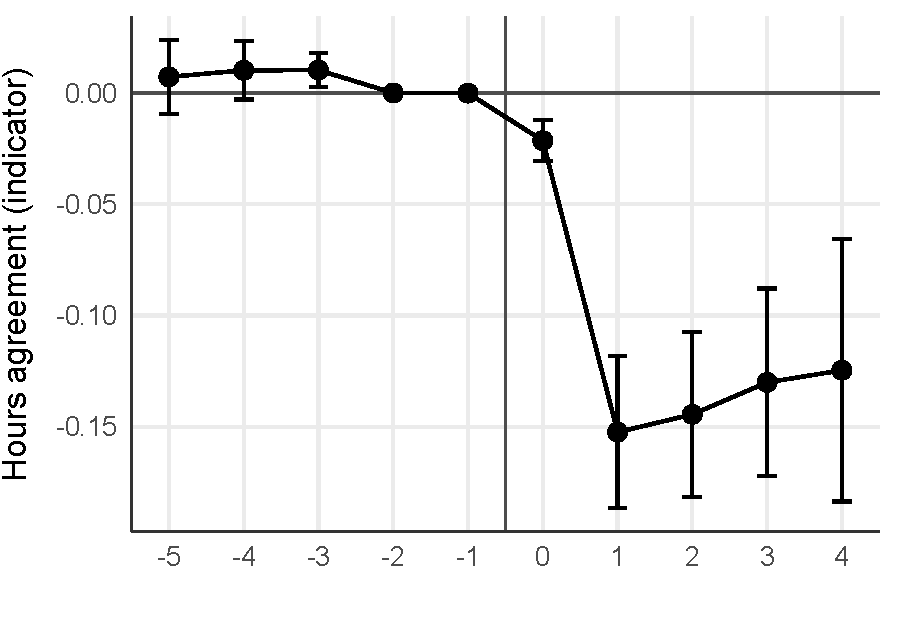
\includegraphics[width=\linewidth,max width=\linewidth]{figures/01_event_figures/figure_A21_c_hours_indicator.pdf}
	\end{subfigure}

	\floatfoot{{\footnotesize \textsc{Notes}: Event-study coefficients $\beta_d$ from equation~(\ref{eq:main_estimating_equation}) for three collective-agreement outcomes corresponding to columns~(1), (2) and~(4) of Table~\ref{tab:nego:LEnego_acc_result}. \textbf{Sample}: LE workers displaced after 2007 and their matched controls (the accords sub-sample); firm-level negotiation outcomes are measured over 2005--2007. \textbf{Specification}: baseline (no controls), reference period $d=-1$. Vertical bars denote 99\% confidence intervals based on robust standard errors clustered at the worker level.}}
\end{figure}


\begin{table}[h]
	\caption{Agreements robustness}	\label{tab:nego:LEnego_acc_rob}
	\begin{center}
{\footnotesize\begin{adjustbox}{max width=\linewidth}
\begin{tabular}{l|lllllll}\toprule
		% Generated from current results_analysis CSV files by master.R, section I (scripts/I-PLOTS_AND_TABLES).
% Table A19; status: ready
% Column 4 is acco_isin. Empty legacy lnsize coefficient row omitted because control coefficients are not exported.
% -- means a requested statistic is unavailable; an empty cell means not applicable.
 & (1) & (2) & (3) & (4) \\
Time to displ. & Wage agreement ind. & Wage agreement ind. & Wage agreement ind. & Wage agreement ind. \\
\midrule
$d=-3$ & 0.018 & 0.003 & 0.003 & 0.021 \\
 & (0.003) & (0.002) & (0.002) & (0.003) \\
$d=-2$ & REF & REF & REF & REF \\
 &  &  &  &  \\
$d=-1$ & -0.000 & -0.001 & -0.001 & -0.001 \\
 & (0.001) & (0.001) & (0.001) & (0.001) \\
$d=0$ & -0.014 & -0.010 & -0.011 & -0.023 \\
 & (0.004) & (0.003) & (0.003) & (0.004) \\
$d=1$ & -0.061 & -0.096 & -0.100 & -0.080 \\
 & (0.013) & (0.015) & (0.015) & (0.014) \\
$d=2$ & -0.059 & -0.088 & -0.092 & -0.083 \\
 & (0.014) & (0.017) & (0.016) & (0.015) \\
$d=3$ & -0.071 & -0.098 & -0.102 & -0.097 \\
 & (0.016) & (0.019) & (0.019) & (0.017) \\
$d=4$ & -0.059 & -0.063 & -0.070 & -0.081 \\
 & (0.022) & (0.028) & (0.028) & (0.023) \\
\midrule
Individuals & 28,198 & 28,198 & 28,198 & 27,650 \\
\# treated & 16,597 & 16,597 & 16,597 & 16,376 \\
Legal size bins (4) &  &  & $\surd$ &  \\

		\bottomrule
\end{tabular}
\end{adjustbox}}			
		%\input{03_Draft/tables/LEnego_acc_rob.tex}  
		\floatfoot{{\footnotesize \textsc{Notes}: This table presents event-study estimates of the reallocation of workers displaced for economic reason (LE) across firms with different approach to collective agreement ---see equation (\ref{eq:main_estimating_equation}) and associated text for more details on the specification. \textbf{Comment on timing}: Firm-level outcomes are computed over the 2005-2007 period. To limit the risk of reverse causality we restrict our sample to individuals displaced after 2007. We thus do not observe individuals after $t^D+4$. Accordingly, event-study coefficients reflect the movement of displaced workers to firms with different initial characteristics and \textit{not} changes within-firm in such characteristics. \textbf{Specification}: Column (1) replicates the first column of Table \ref{tab:nego:LEnego_acc_result}. Column (2) adds a control for the logarithm of employers' number of employee to our main equation. Column (3) further adds a fixed effect for four size categories (from 0 to 10, from 11 to 49, from 50 to 299 and above 299 employees). Finally column (4) transforms the outcome of interest by ignoring those firms that are never observed in the agreement database. \textbf{Outcomes}: Table \ref{apptab:definitions} summarizes variables' definition. Wage agreement indicator is an indicator taking value 1 if the firm has signed (at least) one agreement relative to wages over the period. Details are given in \ref{appsec:accord_data}. \textbf{Standard errors}: robust standard errors clustered at the worker-level.}}
	\end{center}
\end{table}


\begin{table}[h] 
\caption{Election results} \label{tab:nego:LEnego_ele_result}
\begin{center}
{\footnotesize\begin{adjustbox}{max width=\linewidth}
\begin{tabular}{l|lll}\toprule
	% Generated from current results_analysis CSV files by master.R, section I (scripts/I-PLOTS_AND_TABLES).
% Table A20; status: ready
% Failed elections follow the paper definition: shinscrit_carence_siren0912.
% -- means a requested statistic is unavailable; an empty cell means not applicable.
 & (1) & (2) & (3) \\
Time to displ. & Average turnout & Failed (\% workers) & CGT (\% workers) \\
\midrule
$d=-3$ & -0.007 & -0.002 & 0.003 \\
 & (0.001) & (0.001) & (0.002) \\
$d=-2$ & REF & REF & REF \\
 &  &  &  \\
$d=-1$ & 0.000 & 0.000 & -0.000 \\
 & (0.000) & (0.000) & (0.000) \\
$d=0$ & -0.018 & -0.000 & 0.009 \\
 & (0.002) & (0.002) & (0.002) \\
$d=1$ & -0.170 & 0.002 & 0.093 \\
 & (0.010) & (0.009) & (0.012) \\
$d=2$ & -0.139 & 0.017 & 0.067 \\
 & (0.010) & (0.010) & (0.013) \\
$d=3$ & -0.115 & 0.019 & 0.052 \\
 & (0.010) & (0.010) & (0.013) \\
$d=4$ & -0.097 & 0.032 & 0.045 \\
 & (0.011) & (0.011) & (0.014) \\
$d=5$ & -0.089 & 0.036 & 0.040 \\
 & (0.012) & (0.012) & (0.015) \\
$d=6$ & -0.088 & 0.043 & 0.044 \\
 & (0.013) & (0.013) & (0.017) \\
\midrule
Individuals & 29,971 & 29,971 & 29,971 \\
\# treated & 17,071 & 17,071 & 17,071 \\
 
	\bottomrule
\end{tabular}
\end{adjustbox}}	
\floatfoot{{\footnotesize \textsc{Notes}: This table presents event-study estimates of the reallocation of workers displaced for economic reason (LE) across firms with different professional election turnout ---see equation (\ref{eq:main_estimating_equation}) and associated text for more details on the specification. \textbf{Comment on timing}: Firm-level outcomes are computed over the 2009-2012 period. Because of a risk of reverse causality, we perform robustness checks in Table \ref{tab:nego:LEnego_ele_rob}. Because we fix firm-characteristics over time, event-study coefficients reflect the movement of displaced workers to firms with different initial characteristics and \textit{not} changes within-firm in such characteristics. \textbf{Outcomes}: Table \ref{apptab:definitions} summarizes variables' definition. Average turnout is at elections held by the firm between 2009-2012 (worker-weighted). Failed is share of workers covered by a failed election. CGT is the share of workers covered by a (potential) CGT DS representative. Details are given in \ref{appsec:elec_data}. \textbf{Standard errors}: robust standard errors clustered at the worker-level.}}
\end{center}
\end{table}

\begin{table}[h] 
\caption{Election robustness}\label{tab:nego:LEnego_ele_rob}
\begin{center}
{\footnotesize\begin{adjustbox}{max width=\linewidth}
\begin{tabular}{l|lll}\toprule
		% Generated from current results_analysis CSV files by master.R, section I (scripts/I-PLOTS_AND_TABLES).
% Table A21; status: ready
% Column 3: log size + legal size bins. Column 4: sample: lowest quartile of layoff share, at cutoff0.00671140939597315
% -- means a requested statistic is unavailable; an empty cell means not applicable.
 & (1) & (2) & (3) & (4) \\
Time to displ. & Average turnout & Average turnout & Average turnout & Average turnout \\
\midrule
$d=-3$ & -0.007 & -0.006 & -0.005 & -0.002 \\
 & (0.001) & (0.001) & (0.001) & (0.001) \\
$d=-2$ & REF & REF & REF & REF \\
 &  &  &  &  \\
$d=-1$ & 0.000 & 0.000 & 0.000 & 0.000 \\
 & (0.000) & (0.000) & (0.000) & (0.000) \\
$d=0$ & -0.018 & -0.017 & -0.016 & -0.009 \\
 & (0.002) & (0.002) & (0.002) & (0.002) \\
$d=1$ & -0.165 & -0.158 & -0.152 & -0.202 \\
 & (0.010) & (0.009) & (0.009) & (0.013) \\
$d=2$ & -0.136 & -0.130 & -0.125 & -0.165 \\
 & (0.010) & (0.010) & (0.010) & (0.014) \\
$d=3$ & -0.112 & -0.108 & -0.105 & -0.142 \\
 & (0.010) & (0.010) & (0.010) & (0.016) \\
$d=4$ & -0.095 & -0.090 & -0.087 & -0.113 \\
 & (0.011) & (0.011) & (0.011) & (0.017) \\
$d=5$ & -0.086 & -0.082 & -0.080 & -0.103 \\
 & (0.012) & (0.012) & (0.012) & (0.019) \\
$d=6$ & -0.084 & -0.080 & -0.078 & -0.111 \\
 & (0.013) & (0.013) & (0.013) & (0.022) \\
\midrule
Individuals & 29,971 & 29,971 & 29,971 & 7,953 \\
\# treated & 17,071 & 17,071 & 17,071 & 4,144 \\
Legal size bins (4) &  &  & $\surd$ &  \\

		\bottomrule
\end{tabular}
\end{adjustbox}}
%\scalebox{.8}{\input{03_Draft/tables/LEnego_ele_rob.tex}}
\floatfoot{{\footnotesize \textsc{Notes}: This table presents event-study estimates of the reallocation of workers displaced for economic reason (LE) across firms with different professional election turnout ---see equation (\ref{eq:main_estimating_equation}) and associated text for more details on the specification. \textbf{Comment on timing}: Firm-level outcomes are computed over the 2009-2012 period. We perform robustness checks in this table. Because we fix firm-characteristics over time, event-study coefficients reflect the movement of displaced workers to firms with different initial characteristics and \textit{not} changes within-firm in such characteristics. \textbf{Outcomes}: Table \ref{apptab:definitions} summarizes variables' definition. Average turnout is at elections held by the firm between 2009-2012 (worker-weighted). Details are given in \ref{appsec:elec_data}. \textbf{Specifications}: Column (1) replicates the first column of Table \ref{tab:nego:LEnego_ele_result}. Column (2) replicates column (1) but controlling for firm size. Column (3) estimates the effect on a sub-sample made of the quarter of laid-off workers that were part of the smallest layoff (as a share of firm employment). \textbf{Standard errors}: robust standard errors clustered at the worker-level.}}
\end{center}
\end{table}


%\FloatBarrier
%%
%%\section{Miscellaneous\label{appsec:others}}
%%\input{appendix/others.tex}



\end{document}


